\documentclass[11pt,twoside,openright]{report}
% ---------------------------------------------------------------------------
% Shared preamble: fonts, palette, page, floats, code listings, cross-refs.
% Built with pdflatex. Libertinus carries the body, its sans the headings and
% figure furniture, and Inter's mono the JSON and the endpoints.
% ---------------------------------------------------------------------------

\usepackage[T1]{fontenc}
\usepackage[utf8]{inputenc}
\usepackage{libertinus-type1}
\usepackage[scaled=0.82]{beramono}
\usepackage{microtype}
\usepackage{amsmath}

\usepackage[
  a4paper,
  top=28mm, bottom=28mm, inner=30mm, outer=26mm,
  marginparwidth=0mm, footskip=14mm
]{geometry}

\usepackage{graphicx}
\usepackage{xcolor}
\usepackage{booktabs}
\usepackage{tabularx}
\usepackage{longtable}
\usepackage{multirow}
\usepackage{array}
\usepackage{float}
\usepackage{caption}
\usepackage{subcaption}
\usepackage{enumitem}
\usepackage{fancyhdr}
\setlength{\headheight}{14pt}
\usepackage{titlesec}
\usepackage{listings}
\usepackage{tikz}
\usepackage{pgfplots}
\pgfplotsset{compat=1.18}
\usetikzlibrary{positioning,arrows.meta,calc,fit,backgrounds,shapes.geometric}

\usepackage[hidelinks]{hyperref}
\usepackage[nameinlink]{cleveref}

% --- palette -----------------------------------------------------------------
% One ink, one accent, and a muted categorical set. The categorical colours are
% ordered so that adjacent series stay distinguishable in greyscale.
\definecolor{ink}       {HTML}{1A1D21}
\definecolor{ink60}     {HTML}{5B6169}
\definecolor{ink30}     {HTML}{9AA1A9}
\definecolor{rule}      {HTML}{D8DBDF}
\definecolor{paper}     {HTML}{FFFFFF}
\definecolor{wash}      {HTML}{F4F5F7}
\definecolor{accent}    {HTML}{1F5C8B}
\definecolor{accentsoft}{HTML}{DCE8F1}

\definecolor{catA}{HTML}{1F5C8B}
\definecolor{catB}{HTML}{C86A3A}
\definecolor{catC}{HTML}{4C7A4A}
\definecolor{catD}{HTML}{8A5A93}
\definecolor{catE}{HTML}{B03A48}
\definecolor{catF}{HTML}{6E7A86}

% The two parties the paper is about, given one colour each and used nowhere else.
\definecolor{studioC}{HTML}{1F5C8B}
\definecolor{agentC} {HTML}{C86A3A}

\hypersetup{
  colorlinks=false,
  pdfborder={0 0 0},
  bookmarksnumbered=true
}

% --- headings ----------------------------------------------------------------
\titleformat{\chapter}[display]
  {\normalfont\sffamily\bfseries}
  {\color{ink30}\normalsize\MakeUppercase{\chaptertitlename}\ \thechapter}
  {6pt}
  {\Huge\color{ink}}
\titlespacing*{\chapter}{0pt}{0pt}{26pt}

\titleformat{\section}{\normalfont\sffamily\large\bfseries\color{ink}}{\thesection}{0.7em}{}
\titleformat{\subsection}{\normalfont\sffamily\normalsize\bfseries\color{ink}}{\thesubsection}{0.7em}{}
\titleformat{\subsubsection}{\normalfont\sffamily\small\bfseries\color{ink60}}{}{0em}{}

\setlength{\parskip}{0pt}
\setlength{\parindent}{1.2em}
\linespread{1.06}

% --- headers -----------------------------------------------------------------
\pagestyle{fancy}
\fancyhf{}
\renewcommand{\headrulewidth}{0.4pt}
\renewcommand{\headrule}{\hbox to\headwidth{\color{rule}\leaders\hrule height \headrulewidth\hfill}}
\fancyhead[LE]{\footnotesize\sffamily\color{ink60}\leftmark}
\fancyhead[RO]{\footnotesize\sffamily\color{ink60}\rightmark}
\fancyfoot[C]{\footnotesize\sffamily\color{ink60}\thepage}
\fancypagestyle{plain}{\fancyhf{}\renewcommand{\headrulewidth}{0pt}%
  \fancyfoot[C]{\footnotesize\sffamily\color{ink60}\thepage}}

% --- captions ----------------------------------------------------------------
\captionsetup{
  font={small},
  labelfont={sf,bf,color=ink60},
  textfont={color=ink},
  labelsep=period,
  justification=raggedright,
  singlelinecheck=false,
  skip=7pt
}
\captionsetup[sub]{font={footnotesize},labelfont={sf,color=ink60}}

% --- tables ------------------------------------------------------------------
\renewcommand{\arraystretch}{1.22}
\setlength{\tabcolsep}{6pt}
\newcolumntype{L}[1]{>{\raggedright\arraybackslash}p{#1}}
\newcolumntype{R}[1]{>{\raggedleft\arraybackslash}p{#1}}
\newcolumntype{Y}{>{\raggedright\arraybackslash}X}

% A monospaced cell for rule ids, endpoints and field names.
\newcommand{\id}[1]{{\ttfamily\small #1}}
\newcommand{\route}[1]{{\ttfamily\small #1}}

% --- code --------------------------------------------------------------------
\lstdefinelanguage{json}{
  morestring=[b]",
  showstringspaces=false,
  literate=
    *{\{}{{{\color{ink60}\{}}}{1}
     {\}}{{{\color{ink60}\}}}}{1}
     {[}{{{\color{ink60}[}}}{1}
     {]}{{{\color{ink60}]}}}{1}
     {:}{{{\color{ink60}:}}}{1}
     {,}{{{\color{ink60},}}}{1}
}
\lstset{
  basicstyle=\ttfamily\footnotesize\color{ink},
  stringstyle=\color{accent},
  commentstyle=\color{ink30}\itshape,
  keywordstyle=\color{catC}\bfseries,
  numbers=none,
  frame=single,
  rulecolor=\color{rule},
  framesep=7pt,
  xleftmargin=2pt,
  xrightmargin=2pt,
  backgroundcolor=\color{wash},
  breaklines=true,
  breakatwhitespace=true,
  columns=fullflexible,
  keepspaces=true,
  aboveskip=11pt,
  belowskip=11pt
}
\lstdefinestyle{shell}{language=bash,backgroundcolor=\color{wash},keywordstyle=\color{ink}}

% --- an aside box, for a ruling or a trap ------------------------------------
\newenvironment{ruling}[1]
  {\par\medskip\noindent\begin{tikzpicture}\node[
      draw=accentsoft, line width=0.9pt, fill=accentsoft!35, rounded corners=1pt,
      inner sep=9pt, text width=\dimexpr\linewidth-22pt\relax, align=left]\bgroup
      \begin{minipage}{\dimexpr\linewidth-22pt\relax}
      {\sffamily\bfseries\small\color{accent} #1}\par\smallskip\small}
  {\end{minipage}\egroup;\end{tikzpicture}\par\medskip}

\newcommand{\studio}[1]{\textcolor{studioC}{\textbf{#1}}}
\newcommand{\agent}[1]{\textcolor{agentC}{\textbf{#1}}}

% --- generated facts ----------------------------------------------------------
% Totals measured off the running studio, so the prose cites the measurement
% rather than a literal. Regenerated with the rest of data/.
%% Generated from the running pgm-studio API (http://localhost:7894/api) --- do not edit by hand.
%% Source: GET /api/rules, GET /api/rules/terms, GET /api/openapi/v1.json, /home/user/pgm-studio/docs/generator/rules.md
% A family is the family field the API answers with, not the rule id's prefix:
% four build-zone rules are numbered BZ and belong to family CT, so the ids carry
% 29 prefixes across 28 families.
% The law counts are parsed from the document itself: Law*Count is its id bullets
% and its family headings, LawIdPrefixCount the prefixes those ids span (BZ has
% ids under no heading of its own), LawServedCount the law ids GET /api/rules answers.
\newcommand{\RuleCount}{183}
\newcommand{\RuleFamilyCount}{28}
\newcommand{\RuleIdPrefixCount}{29}
\newcommand{\ScoredTermCount}{31}
\newcommand{\RouteCount}{231}
\newcommand{\RoutePathCount}{174}
\newcommand{\RouteAreaCount}{22}
\newcommand{\LargestFamily}{SK}
\newcommand{\LargestFamilyCount}{28}
\newcommand{\LawRuleCount}{97}
\newcommand{\LawFamilyCount}{12}
\newcommand{\LawIdPrefixCount}{13}
\newcommand{\LawServedCount}{41}



\title{How a PGM Map Gets Made}
\author{}
\date{}

\begin{document}

\thispagestyle{empty}

\begin{center}
\vspace*{2.2cm}

{\sffamily\fontsize{34}{38}\selectfont\bfseries\color{ink} How a PGM Map\\[2pt] Gets Made}

\vspace{14pt}
{\color{rule}\rule{0.32\textwidth}{1.1pt}}
\vspace{14pt}

{\sffamily\large\color{ink60} The division of labour between an authoring agent\\ and \textsf{pgm-studio}}

\vspace{2.4cm}

\begin{minipage}{0.76\textwidth}
\small\color{ink}
Two maps are built from first principles in these pages: a Capture the Wool
board, composed by the studio and then adapted into a place, and a
destroy-the-monument board authored from nothing at all. Every stage of both is
shown as it came out of the machine. At each stage the paper asks the same
question. \emph{Who decided this?}
\end{minipage}

\vfill

{\footnotesize\sffamily\color{ink60}
Written from the running studio, September 2026\par}

\vspace{1.2cm}
\end{center}

\clearpage

% ---------------------------------------------------------------------------
\thispagestyle{empty}
\vspace*{1cm}

\section*{Purpose, Audience and Method}
\addcontentsline{toc}{chapter}{Purpose, Audience and Method}

\noindent
\textsf{pgm-studio} is a program for making Minecraft PvP maps of the kind a PGM
server loads. It is driven over HTTP, which means the thing operating it need not
be a person sitting at a screen. For most of the maps described here, the operator
was a language model with a terminal and a list of endpoints. This paper is an
account of what such a machine actually does, and of what the studio does for it.

\medskip\noindent
That question turns out to be the interesting one. A map is not produced by a
generator that takes a seed and returns a finished world, and it is not produced
by an author typing coordinates either. It is produced by two parties handing work
back and forth, and the line between them moves from stage to stage. The studio
arranges a board and the agent decides what the ground is. The agent states a
theme and the studio decides which block lands on which cell. The agent asks for
something, the studio refuses, and the refusal is where a good deal of the map
comes from. Naming that line precisely, stage by stage, is the whole of what
follows.

\medskip\noindent
The paper is in three parts, and they can be read in any order.

\begin{description}[leftmargin=1.6em,style=nextline,itemsep=5pt]
  \item[Part~I. The System] What a map is made of, the four documents that
    describe one, and the division of labour stated plainly. Three short
    chapters; read these first whatever else you read.
  \item[Part~II. The Instruments] One chapter per capability of the studio: the
    composer, the rules, shapes, relief, layers, terrain, houses, dressing, the
    export, reading a world back, and what an agent reads before it starts. This
    is the reference half, meant to be dipped into rather than read through.
  \item[Part~III. Two Maps, End to End] The two boards, every stage pictured, and
    a chapter on what an authoring session actually looks like from the outside,
    reconstructed from a recording of every call the agent made.
\end{description}

\medskip\noindent
A reader who plays these maps and wants to know where they come from can read
Part~I and then Part~III, and skip the middle entirely. A reader who wants to
drive the studio wants Part~II. Terms are defined where they are first used, and
collected again in the glossary at the back.

\medskip\noindent
One discipline is worth stating up front, because it constrains what this paper is
permitted to say. Nothing here claims that a map \emph{plays} a particular way
unless that claim traces to one of two sources: a ruling by the repository's
author, cited as such, or a measurement over the corpus of roughly 350 published
PGM maps, quoted with its number. The source code can say what the software does
and the corpus can say what mapmakers have done. Neither can say what is good.
Where the honest answer was that nobody had measured it, the claim is absent
rather than invented.

\clearpage


\tableofcontents
\cleardoublepage

\chapter{Maps, Objectives and the Two Authors}

\section{The Anatomy of a PGM Map}

PGM is a server plugin that runs competitive Minecraft matches. It loads a map,
which is two things bundled together: a Minecraft world, meaning the blocks, the
terrain and the buildings; and a file called \id{map.xml} that says what the world
is \emph{for}. Without the XML the world is scenery. The XML is what states that
this team spawns here, that this region cannot be built in, that the match ends
when that block is broken.

Objectives come in a handful of kinds, and two of them carry this paper. A
\textbf{Capture the Wool} map, universally abbreviated CTW, hides coloured wool in
rooms, and a team wins by carrying the right wool back to its own monument. A
\textbf{destroy-the-monument} map, DTM, puts a block or a small structure in each
team's ground, and a team wins by breaking the enemy's. Others exist: a core that
leaks lava when broken, a control point held over time. The studio builds them
all, but CTW and DTM are the two worked examples here.

\section{Team Counts by Objective}
\label{sec:team-counts}

The number of teams a map can hold is not one question but two, and they have
different answers. One is about the objective and belongs to PGM. The other is
about symmetry and belongs to the studio.

Capture the Wool works at two teams or four, and four-team CTW maps have been
built. It works at four because each team has a \emph{distinct} objective:
capturing the other three teams' wools. Control points, whose support is recent,
take four teams or more, usually an even number, simply because maps are usually
symmetric.

Destroyables and cores are different, and the reason is worth stating properly
because it is easy to mistake for a software limit. It is not one. The difficulty
is \textbf{ownership}. A destroyable cannot be assigned to a team the way a wool
can. If a team's monument is destroyed then that team has, in a sense, lost. But
that does not determine a \emph{winner}, and with more than two teams there is no
well-defined one. PGM maps work around it in two ways. Some make the match blitz,
so the last surviving team wins. Others move the players of a team that has lost
its monument onto another team, so that one team can truly win. Neither of those
is raw DTM or DTC. A destroy map without one of those modes layered on it is
therefore a two-team map in practice.

\begin{ruling}{The Studio's Team Ceiling}
The studio's automatic symmetry fan tops out at four teams, because \id{rot\_90}
is the only four-image mode it has. That is what caps the studio, rather than
anything about the objectives. An agent driving the API directly can author
anything, a six-team map included. What it gives up is the automatic fan, so each
team's ground has to be authored rather than mirrored into place.
\end{ruling}

The blocks and the XML have to agree with each other, and that is harder than it
sounds. A wool room's position in the XML is a coordinate; whether that coordinate
is inside a room a player can reach is a fact about the blocks. A build region
drawn in the XML means nothing if the ground it covers was never placed. Most of
what a map-authoring program does is keeping those two descriptions true of one
another.

\section{The Studio: Scope and Interface}

\textsf{pgm-studio} is an ASP.NET Core application with a browser client, a
database, and an HTTP API of \RoutePathCount{} paths carrying \RouteCount{}
operations. It authors maps: it plans a layout, draws its ground, states what the
map is played for, and writes out the world and the \id{map.xml} a server can
load.

The browser client exists and is used. But the API is the whole surface, and every
map described in this paper was made without opening the client once. A caller
with a terminal can compose a board, reshape its ground, state its objectives,
build the world and read the result back, entirely over HTTP. That property is
what makes the rest of this paper possible, and it was designed in rather than
discovered. The documentation for each tool carries that tool's endpoints, on the
principle that a description which cannot be acted on is a description of nothing.

\section{The Authoring Agent}

For most of the maps in the repository this paper draws on, the operator is a
language model running in a terminal. It reads documentation, writes a Python
script that emits two JSON documents, posts them, reads the studio's answer and
corrects. It has no eyes on the world. It cannot walk around the map. Every belief
it holds about what it has built comes from a number the studio handed back, and a
good deal of the discipline described in Part~III exists because that is a
genuinely difficult position to author from.

This paper calls that operator \agent{the agent} throughout, and the program it
drives \studio{the studio}. The two words are used precisely and always mean those
two things.

\section{The Central Argument}

It is tempting to describe a system like this as a generator with a human in the
loop, or as an editor with some automation in it. Neither is right, and the reason
neither is right is the substance of this paper.

The studio is not a generator, because it does not produce maps. Its composer
produces an \emph{arrangement}: where the hub sits, how far the wool rooms stand
off it, which side the front line faces. An arrangement is not a map. It has no
elevation, no curve, no building, no second storey, no material. Every composed
board is flat, rectangular and grey. What it buys is the one thing that is hard to
invent and easy to get wrong, and the repository's own brief on the subject puts it
as sharply as it can be put: a composed board is a suggestion, not a plan.

The studio is not an editor either, because a very large amount of what ends up in
the world was never stated by the agent. The agent says a theme should follow the
ground's slope, and the studio decides which of five materials lands on each of
several hundred thousand cells. The agent says a house stands here, and the studio
decides its storey heights, its roof pitch, where its door goes and which way the
door faces. The agent says the two halves of the board are mirror images, and the
studio decides what that means for every shape, every prop and every region. These
are not defaults in the sense of values that could have been typed out. They are
derivations, and the agent could not have produced them by hand in any reasonable
time.

The honest description is therefore the third one: two parties, a boundary between
them, and the boundary in a different place at every stage. At the board level the
studio arranges and the agent adapts. At the ground level the agent states intent
and the studio computes geometry. At the paint level the agent picks a rule and the
studio applies it. At the objective level the agent decides almost everything, and
the studio's task is to refuse the decisions that cannot be built.

That last one deserves its own sentence, because it is the part least visible from
outside. A large fraction of the studio consists of gates: \RuleCount{} rules
across \RuleFamilyCount{} families, each of which can stop a request and say why.
They are not validation in the defensive sense. They are the accumulated knowledge
of what makes a map fail, expressed as things the software will not let happen, and
an agent authoring against them is being taught as much as it is being checked.

\section{Structure of This Paper}

The paper works through the stack once, in the order a map passes through it, and
at each stage says which party decided what. Then it builds two maps.

The first is a CTW board in the \emph{micro} size band, pulled straight off the
composer and then adapted: reshaped, given elevation, given buildings, given a
second storey, until it is a place rather than a diagram. The second is a DTM
board authored from nothing, with no composed arrangement to start from, by an
agent given no brief beyond the objective. Both are shown at every stage of the
pipeline, from the bare rectangles the composer emitted to the finished world.

The last chapter is about the agent rather than the map. While the DTM board was
being authored, every HTTP call its author made was recorded: the route, the
status, the rules that fired, the time it took. That recording is what the chapter
is written from, so the account of how an authoring session goes is taken off the
wire rather than from the agent's own description of itself.

\chapter{The Four Levels of Description}
\label{ch:four-levels}

\section{A Map as Four Documents}

The first thing to understand about the studio is that it does not hold a map. It
holds four descriptions of one, at four different grains, each owned by a
different tool and stored separately. The documentation states it flatly:

\begin{quote}
A map is not one document. It is four, each describing the whole map at a
different grain, each owned by a different tool and stored separately.
\end{quote}

\Cref{tab:levels} is that list. Read it top to bottom as increasing resolution:
the board knows what things are and not where they are exactly; the world knows
where every block is and nothing about what any of it is for.

\begin{table}[htbp]
\caption{The four levels. Each is a description of the whole map.}
\label{tab:levels}
\small
\begin{tabularx}{\textwidth}{L{2.1cm} Y L{3.1cm} L{1.9cm}}
\toprule
\textbf{Level} & \textbf{What it states} & \textbf{Document} & \textbf{Tool} \\
\midrule
The board &
  Rectangles on a coarse cell grid, what each one is for, and where the
  objectives sit &
  \id{PlanModel} \newline (\id{*.plan.json}) & Plan \\
The ground &
  The real geometry at block resolution: outlines, heights, relief, paint, props &
  \id{SketchLayout} & Sketch \\
The play &
  Teams, spawns, protections, build regions, objectives and how they are captured &
  \id{MapIntent} & Configure \\
The map &
  The voxel world and the \id{map.xml} a PGM server loads &
  \id{VoxelWorld} + \id{MapXml} & --- (built) \\
\bottomrule
\end{tabularx}
\end{table}

\subsection*{These are grains, not drafts}

The temptation is to read the four as stages of completeness, a rough sketch
refined into a finished thing. That reading is wrong and leads directly
to authoring mistakes, so the documentation heads it off:

\begin{quote}
A plan is not a rough draft of a layout: it states things a layout cannot, such as
that this rectangle is a wool room, or that these two pieces share a defence wall,
and cannot state things a layout can, like a curve or a one-block step. The same is
true upward: a layout knows where every block of ground is and has no idea what
any of it is for. That is why a finished map needs all four and why no one of them
is `the' map.
\end{quote}

This is worth dwelling on because it explains the shape of everything downstream.
A wool room is a concept that only exists at the board level. Once the board
compiles, there is no wool room in the geometry. There is a polygon, at a height,
with a theme on it. Conversely a coastline is a concept that only exists
at the ground level; no arrangement of rectangles can state one. An agent that
tries to express a curve in the plan is fighting the model, and an agent that
tries to state an objective in the layout is doing the same thing from the other
side.

\subsection*{The flow is one-way}

\begin{quote}
A plan compiles into a layout and an intent; a layout rasterizes into a world; an
intent projects into the map document; the document writes out as \id{map.xml}.
Nothing reads back up. There is no path from geometry to a plan, and none from a
finished \id{map.xml} to an intent. Both omissions are deliberate.
\end{quote}

Nothing infers upward. A finished map cannot be decompiled into the plan that
would have produced it, and the studio does not try; the documentation's position
is that hypothesising what a finished map's plan would have been is a person's job
rather than a tool's. The practical consequence for an agent is that corrections
are made \emph{upstream and re-run}, not patched downstream. If the ground is
wrong, the thing to change is the document that produced it.

\begin{figure}[htbp]
\centering
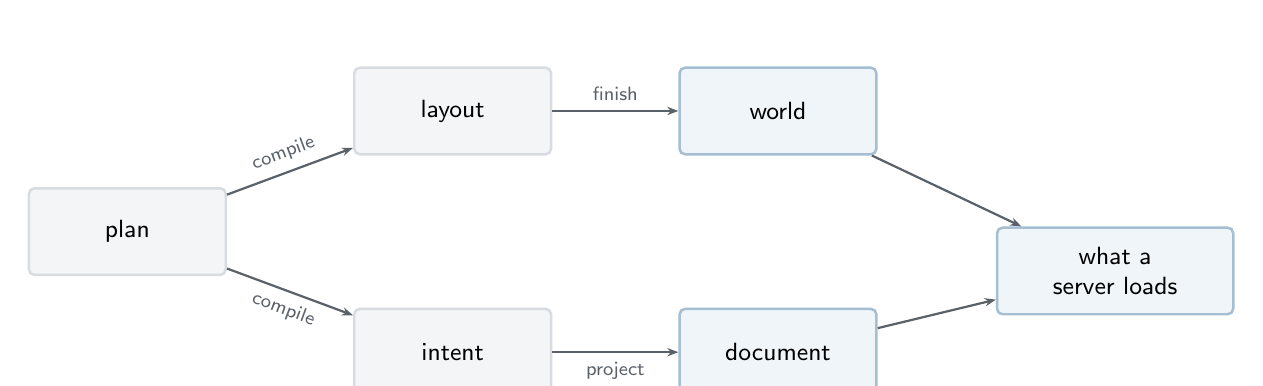
\begin{tikzpicture}[
  font=\sffamily\small,
  doc/.style={draw=rule, line width=0.9pt, fill=wash, rounded corners=2pt,
              minimum height=11mm, minimum width=25mm, align=center, inner sep=4pt},
  built/.style={doc, fill=accentsoft!45, draw=accent!40},
  every path/.style={draw=ink60, line width=0.8pt, -{Stealth[length=4pt]}}
]
\node[doc] (plan) {plan};
\node[doc, above right=4mm and 16mm of plan] (layout) {layout};
\node[doc, below right=4mm and 16mm of plan] (intent) {intent};
\node[built, right=16mm of layout] (world) {world};
\node[built, right=16mm of intent] (document) {document};
\node[built, below right=9mm and 15mm of world, minimum width=30mm] (out) {what a\\ server loads};

\draw (plan) -- node[above, sloped, font=\sffamily\scriptsize, color=ink60] {compile} (layout);
\draw (plan) -- node[below, sloped, font=\sffamily\scriptsize, color=ink60] {compile} (intent);
\draw (layout) -- node[above, font=\sffamily\scriptsize, color=ink60] {finish} (world);
\draw (intent) -- node[below, font=\sffamily\scriptsize, color=ink60] {project} (document);
\draw (world) -- (out);
\draw (document) -- (out);
\end{tikzpicture}
\caption{The five hand-offs. The two branches rejoin at the end rather than
staying independent: building the world \emph{resolves} parts of the intent, and
the \id{map.xml} is rendered from that resolved copy.}
\label{fig:handoffs}
\end{figure}

\section{The Five Hand-Offs}

\Cref{fig:handoffs} is the whole pipeline. Each arrow is a call.

\paragraph{Plan to layout and intent.} \route{POST /api/plan/compile} turns one
plan into both downstream documents, and it is pure: the same plan compiles to the
same pair on the server and in the browser. One thing happens here that surprises
people reading a compiled board for the first time. Abutting pieces of equal
height fuse into single polygons, so what arrives at the ground level is a board
rather than a grid of rectangles. A plan of eleven rectangles can compile to four
shapes.

\paragraph{Layout onto a map.} \route{PUT /api/map/\{slug\}/sketch/from-plan}
merges rather than replaces. Themes, room shells, dressing and author-corrected
heights are carried onto the fresh geometry. Relief is the exception, and the
reason is worth stating because it is the clearest example in the system of the
studio refusing to guess: relief is keyed by group id, group identity is derived
from the geometry, and a recompile that re-fuses the board produces different
groups. Hand-authored terrain would have nowhere correct to land. So that case
answers \textbf{409}, one \id{SK1} finding per group it would orphan, and
\id{?force=true} accepts the loss. It is the author's call, not the server's.

\paragraph{Intent onto a map.} \route{PUT /api/map/\{slug\}/intent/from-plan}
carries much less: the authors and contributors the stored intent already held,
and nothing else. Two slices deliberately do not ride across. \id{islandTeams} is
a positional derivation, and carrying it would relabel territory rather than
preserve an answer. \id{symmetry} is left behind because its presence is what
switches the orbit expander on. A rebuild therefore clears both, and the World and
Teams phases have to be walked again.

\paragraph{Layout to world.} \route{POST /api/map/\{slug\}/sketch/finish}
rasterizes the layout into world geometry and moves the map to the configure
stage. This is the only stage transition the studio performs at runtime.

\paragraph{Intent to document to \id{map.xml}.} \route{PUT /api/map/\{slug\}/intent}
stores the intent and projects it into the PGM document (teams, kits, regions,
filters, apply-rules and spawns) in one idempotent pass.
\route{GET /api/map/\{slug\}/xml} renders that document;
\route{GET /api/map/\{slug\}/export} gives the world.

\section{The Three-Document Load}

An agent reading the five hand-offs might reasonably conclude that authoring a map
means making five calls in order. It does not, and this is the single most
consequential piece of practical knowledge in the whole pipeline.

\route{POST /api/map/from-documents} takes a plan, a layout and an intent
together, stores a whole map from them, and answers the slug it landed under. The
compile, the rasterize and the projection all run inside it. A map already stored
under that slug is replaced, because the documents name one map, so loading them
twice is a reload rather than a second map.

The documentation is explicit that this is the authoring call and not merely the
import one, and equally explicit about what the staged path costs an agent that
walks it instead: six calls for one store, a fresh slug originated on every
correction, and the need to know that the intent's projection lands after the
metadata write. The staged path is what the browser does. A driver never needs it.

The layout and the intent are required; the plan is not. A board drawn on a grid
has no plan, so a layout emitter states none. Omitting either of the required two
answers \textbf{400} naming which.

This call is also the way \emph{back} in, and that matters more than it sounds.
No route in the studio reads a \id{map.xml} at all: \route{POST /map/import-folder}
refuses a folder carrying one outright, and \route{import-url} extracts only the
region files. So a map authored against one studio could reach another only as a
world, arriving without its plan, its drawing or its intent, and never able to be
re-planned. The three documents carry more than the world does.

\begin{ruling}{Request Body Conventions}
Twenty-five of the studio's write endpoints take a bare document and fourteen take
a wrapper, so an author guessing gets it right slightly more than half the time.
The rule that resolves it: if the endpoint is asking \emph{about a document}, post
the document unwrapped; if it is asking to \emph{file a document under a name},
post the record that names it. A wrong guess is silent, because an unknown
property is dropped rather than reported. Posting \id{\{"style": \{...\}\}}
where a bare style was wanted answers \textbf{200} with a preview of the defaults.
\end{ruling}

\section{The Library}

Beside the four sits one more thing that is not a level at all: the library of
materials, themes, house parts and room styles. It knows nothing about maps, having
neither slug nor stage, and the tools that build worlds reach into it to pick a
recipe.
What they take is a \emph{copy}, so a library edit can never rebuild a map that
already shipped. A theme changed today does not alter a world exported last week.

\section{Stage and Layer}

A map row carries a \textbf{stage} and, separately, the \textbf{layers} it holds.
A stage is where a map has got to. A layer is a document it carries, and it keeps
carrying it: a map built from a plan still has its plan after it has been
sketched, configured and exported.

A stage is a progress marker and not a lock. A configured map may be re-planned,
and no endpoint refuses on the basis of the stage a map stands at. What the stage
is for is saying which of the moves already open is the one the author was about
to make.

The studio answers both questions at runtime.
\route{GET /api/map/\{slug\}/state} gives the stage, the artifacts, and the moves
they allow, each with its route. A move is offered because the documents it reads
are stored, not because the stage is right. Its pair,
\route{GET /api/map/\{slug\}/findings}, answers what is wrong with the map right
now from every gate the stored documents can reach, and names the gates it did
\emph{not} ask along with the route that pays for them. An agent that has lost
track of where it is asks those two.

\section{Responsibilities Held at a Single Level}

A few things belong to exactly one level, and an agent looking for them at the
wrong one will not find them.

Terrain paint and dressing are the ground level's alone. The rasterizer is what
makes the world, so a finish authored a level above it would be authored before
the thing it finishes exists. The observer spawn is the play level's alone: a plan
puts it at the origin at a computed height, which is why an unattended spectator
stands at $0,0$. Water lanes are the board level's alone; they survive a
save at the play level and generate their region, but nothing at that level draws
them. Room shells come from the ground level's theme phase rather than from the
play level, which is the one most often looked for in the wrong place.

\chapter{The Division of Labour}
\label{ch:division}

\section{The Boundary and Its Source}

The repository states its own answer in one sentence, in the brief that governs
authoring from a composed board:

\begin{quote}
A composed board is a \textbf{suggestion}, not a plan.
\end{quote}

And then, more usefully, the mechanism behind it:

\begin{quote}
It emits a plan, not a layout. The plan is where the board's \emph{arrangement}
lives. Everything that makes a place, whether the shape of the ground, the second
storey, the edge that is not a straight line, the wall or the island, is
downstream of it and is yours.
\end{quote}

That is the cleanest statement of the boundary anywhere in the system, and it maps
exactly onto \cref{ch:four-levels}'s four levels. The studio's generative half
works at the board level and stops there. Everything at the ground level, the play
level and the world is authored. That does not mean typed out by hand, because the
studio computes enormous amounts of it, but it does mean that no part of it
happens unless the agent asks for it.

\section{Contributions of the Studio}

\subsection{The Arrangement}

The composer knows how a CTW board is put together: a hub with a spawn hung off
it, one or two wool approaches hanging off the hub's free surface, a frontline
fronting it, a mid band between the two fanned images with a row of stepping
stones in it, and a land budget that keeps a wool board about a third land. The
brief's verdict on why that is worth having is unsentimental. It is the thing that
is hard to invent and easy to get wrong, and a board drawn from scratch that
ignores it comes out illogical in ways no gate catches.

It is equally explicit about where that stops. \Cref{tab:composer-stops} is the
list, and every row of it is a thing the agent must supply or the board will not
have.

\begin{table}[htbp]
\caption{What the composer does not do, and what therefore arrives as the agent's
work. Every row is stated in the repository's own brief.}
\label{tab:composer-stops}
\small
\begin{tabularx}{\textwidth}{L{5.4cm} Y}
\toprule
\textbf{The composer does not} & \textbf{So the board arrives} \\
\midrule
vary the crossing's ground &
  with one lateral row of stones at one depth: no tiered island, no staggered
  pair, nothing off the band's centre line \\
place defence walls &
  \id{"walls": []}, always. A defence wall is authored, never composed \\
state any elevation &
  with no piece carrying a surface; the whole board flat at
  \id{globals.surface}~9 \\
draw anything but rectangles &
  as axis-aligned cell rects, with no curve, no spur and no taper anywhere \\
model an intra-team build zone &
  with exactly one zone, the mid band \\
carry layers &
  with no storeys at all: no bottom lane, no top lane, no tunnel, no undercroft \\
make four-team boards &
  two teams only, whatever is asked for \\
balance its own wools &
  routinely lopsided (\cref{sec:lopsided}) \\
\bottomrule
\end{tabularx}
\end{table}

\subsection{Derived Furniture}

Downstream of the plan, a great deal appears that the agent never wrote. When a
CTW board is stored, the studio works out the monuments, places them beside the
right spawns, and generates the regions, filters and apply-rules that make them
function. One run records the scale of this plainly: a plan stating four wool
rooms and their markers produced four wools, four monuments, 22 regions, 34
filters and 11 apply-rules, with no authoring and no correction.

The same is true of values that are derived rather than placed. The build ceiling
is the tallest terrain column plus twenty, so raising any terrain silently raises
the ceiling over the whole board. A \id{walls} entry names an interface and
nothing else; the studio decides that a wall is bedrock, two thick, three courses,
across the full interface width, stamped on the attack side. Pieces are fanned
through the board's symmetry automatically, though as \cref{ch:refusals} will show,
not everything is, and knowing which is which has cost several runs a rebuild.

\subsection{Substitution and Complaint}

One case is worth isolating because it shows the studio's temperament. A run
specified obsidian for a fifteen-block destroyable, which is out of band. The
studio did not refuse. It built the map in ender stone, raised the complaint
\id{DC3} saying so, and wrote the \id{map.xml} declaring what was actually laid.
A refusal stops the request; a complaint lets it through and states what changed.
That distinction runs through the whole API, and an agent that reads only the
status code throws half the answer away.

\section{Decisions of the Agent}

\subsection{The Identity Sentence}

The most consistently enforced agent decision in the corpus is also the least
technical: before a single shape is drawn, the agent writes one sentence saying
what the board is. The warmup discipline states it as a rule: decide what the
board is about before deciding what it is made of, keep it to one thing, write the
sentence down, and if it cannot be written the board is not ready.

A worked example, from a run that built four boards at once:

\begin{quote}
A sand spit, flat and pale and open nearly everywhere, with one ring of dune on
it that you have to walk round, two tide-worn stones in the middle at a ten-block
grain, and a water lane down the west flank that opens forty-five minutes in.
\end{quote}

This turns out to be load-bearing in a way nobody designed. One orchestrated run
had three agents killed by an interrupt at twenty-eight minutes. Two of them had
written their identity sentences into their reports before authoring, and those
survived. The third had not, and its three remaining identities were lost with it
and had to be invented again. Writing the identity down first is a durability
property as well as a design one.

\subsection{Palette Across a Set}

Where several boards are built together, the agent chooses each board's ground,
built and accent tones against the others, because, as one run puts it, five boards
can each be internally coherent and still be five greys. The reasoning is
recorded per board as a position in a range: one board the brightest and highest
contrast, another the coldest and bluest and lowest contrast.

\subsection{Size}

Every one of the twelve boards in the most recent composed-board runs resized the
card it was pulled from. The composer sizes to its band; the agent sizes to the
place it has decided on.

\subsection{Gameplay Intent Without an Oracle}

This is the category the repository treats most carefully, and it is the reason
this paper is constrained the way it is. Questions about how a map plays are not
derivable from the code or the corpus. Every run report from the first onward
therefore carries a section titled \emph{open gameplay questions, decided without
an oracle}, in which the agent records the judgement it had to make, the answer it
picked, and its confidence. Three real examples:

\begin{quote}
\textbf{How high may a mid island stand over the fronts?} Gallowsholt's causey is
four blocks proud, so a player bridging out of his own front has to place a block
to get onto it. That makes it a prize and makes the first team there hard to
shift. Decided: four.
\end{quote}

\begin{quote}
\textbf{May two wools be the same distance and completely different to raid?}
Longstrand's are 200 and 192 blocks from the enemy's door; one is inside a ring of
dune you must go round and one is on open strand. Decided yes, and it is the thing
I would most like judged.
\end{quote}

\begin{quote}
\textbf{Is a two-block bench across most of a board playable?} \ldots This is the
decision I am least sure of.
\end{quote}

The practice exists because of a specific failure. An earlier run measured that
destroyables and cores float a few blocks above the terrain, reasoned from first
principles that this made every generated destroy map unwinnable, and filed and
committed the claim. The measurement was right and the conclusion was invented.
The float is deliberate PGM behaviour and has been from the start, because a core
on the ground cannot leak and a destroyable on the ground is trivially covered.
Neither the corpus nor the code would have corrected it. One question would have.

\section{The Intermediate Category}

Between what the studio supplies and what the agent decides sits a third category,
and it is where the system is most itself.

\subsection{Placement as Query}

An agent's natural instinct is to place things by eye: this tree here, that
boulder there, a bench against the wall. The most recent structure-focused run
records what happens when it does.

\begin{quote}
Every prop I placed by eye was declined. \ldots Everything that shipped came from
\route{POST .../sketch/seats} or the candidate loop. Final tally: 78 placed, 0
declined.
\end{quote}

The studio knows where a prop can stand, because it knows the ground, the
clearance, what else is there and what the passage rules require around a
building. The agent does not, because the agent cannot see. So the productive move is not to place and
be corrected; it is to ask what the legal seats are and choose among them. This
inverts the usual relationship between an author and a tool, and it is the single
most transferable piece of craft in the whole corpus.

\subsection{Instruction by Evaluator}

The studio scores a board against 31 terms, and the scores are not merely a grade.
One run records the evaluator changing a design rather than a document: a monument
authored on an open pan read a goal-distance ratio of 1.875 against the
\id{GO1} band of 3.0--4.0.

\begin{quote}
\ldots which is not a placement error. It is the board saying the goal is in the
contested space rather than a short walk forward of the spawn. Moving it to
the brow gave 3.22 and produced the topology the gameplay documentation describes.
\end{quote}

The agent did not learn a number. It learned what the number was about.

\subsection{Convergence as a Failure Mode}

This is the finding that most deserves to be in a paper about generated maps,
because it is the failure mode of the whole approach and it was caught by
accident.

An orchestrated run put three agents on three different ground families, with no
contact between them. They converged on nearly identical goal geometry: spawn
separation 184 blocks, goal 40.5--44.0 from its own spawn, \id{GO1} between 3.24
and 3.59, lateral offset 11--21. The explanation is not imitation, because there
was none available.

\begin{quote}
\ldots because \id{GO1}'s band of [3.0, 4.0] on a lane-shaped board puts the goal
between $L/5$ and $L/4$ from its own spawn, and the centre line is the cheapest
way to satisfy it.
\end{quote}

A constraint with a cheapest satisfying solution will be satisfied that way by
every author who does not deliberately pay more. The rules that keep bad maps from
being built will, left to themselves, also make good maps resemble each other.
Nothing in the system detects this; it took three independent runs and somebody
noticing.

\subsection{Rules as Band Lookups}

One further finding reframes the rule system entirely, and an agent that does not
know it will generalise wrongly from every board it has built:

\begin{quote}
A rule id is not a fixed constraint: \id{FR6}, \id{G8} and \id{CT12} all read
\textbf{authored bands} whose values depend on what the board is played for, and
three boards of experience on one objective family taught me nothing about the
next.
\end{quote}

This is why the studio publishes \route{GET /api/rules/terms}, so that a driver
can ask what band is enforced on \emph{this} board rather than writing down a
number that was true of the last one.

\section{The Boundary by Stage}

\Cref{tab:division} states the division of labour across the whole pipeline. It is
the table the rest of the paper elaborates, and each of its rows is a chapter in
Part~II.

\begin{table}[htbp]
\caption{Who decides what, by stage. \studio{Blue} is the studio; \agent{orange}
is the agent.}
\label{tab:division}
\small
\begin{tabularx}{\textwidth}{L{2.5cm} Y Y}
\toprule
\textbf{Stage} & \textbf{\studio{The studio decides}} & \textbf{\agent{The agent decides}} \\
\midrule
Arrangement &
  hub, spawn, wool approaches, frontline, mid band, land budget, size band &
  which candidate, and everything the composer does not state \\
Ground shape &
  how outlines fuse, how a bend is drawn, where a relief field goes &
  the identity, the sizes, the reshaping, where two grounds meet \\
Elevation &
  the solved height field from the marks it is given &
  the marks, the grain, the pushes, the scopes \\
Layers &
  the painter's bottom-up order, what a layer occludes &
  how many storeys, what is under what, what is a made thing \\
Paint &
  which material lands on which cell, given a band axis &
  the theme, the axis, where the bands cut \\
Structures &
  storey heights, roof pitch, door side, porch, beams &
  which style, which footprint, which seat from the offered set \\
Dressing &
  the legal seats &
  which seats to take, and the styles \\
Objectives &
  monuments, regions, filters, apply-rules, resolved volumes &
  what the map is played for, and where the goals sit \\
Refusal &
  what may not be built, and why &
  what to do about it \\
\bottomrule
\end{tabularx}
\end{table}

\chapter{The Composer and the Size Ladder}
\label{ch:composer}

\section{Composition: Definition and Verbs}

The studio's documentation refuses the word \emph{generate} for this stage, and
the reason is precision rather than pedantry: the word has been used both for the
whole pipeline and for the narrow step that turns an intent into \id{map.xml}.
There are five verbs, each meaning one thing. \textbf{Emit} fills one box with one
base shape. \textbf{Derive} reads structure back out of geometry. \textbf{Compose}
builds the plan. \textbf{Evaluate} scores a plan. \textbf{Realize} compiles a plan
into a sketch and an intent and exports it.

Emit and derive are a forward/inverse pair, and the fact that they are required to
agree is the shape model's correctness test: composition emits, verification
derives, and a disagreement is a defect in one of them.

The whole of composition is one chain, and it runs in one direction.

\begin{figure}[htbp]
\centering
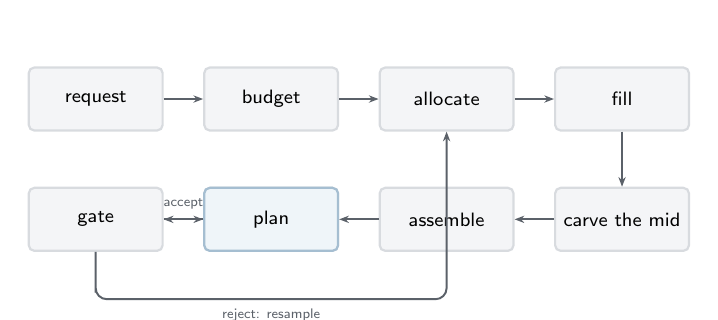
\begin{tikzpicture}[
  font=\sffamily\scriptsize,
  st/.style={draw=rule, line width=0.8pt, fill=wash, rounded corners=2pt,
             minimum height=8mm, minimum width=17mm, align=center, inner sep=3pt},
  every path/.style={draw=ink60, line width=0.7pt, -{Stealth[length=3.5pt]}}
]
\node[st] (req) {request};
\node[st, right=5mm of req] (bud) {budget};
\node[st, right=5mm of bud] (all) {allocate};
\node[st, right=5mm of all] (fil) {fill};
\node[st, below=7mm of fil] (car) {carve the mid};
\node[st, left=5mm of car] (asm) {assemble};
\node[st, left=5mm of asm] (der) {derive};
\node[st, left=5mm of der] (gat) {gate};
\node[st, below=7mm of bud, fill=accentsoft!45, draw=accent!40] (plan) {plan};

\draw (req) -- (bud); \draw (bud) -- (all); \draw (all) -- (fil);
\draw (fil) -- (car); \draw (car) -- (asm); \draw (asm) -- (der); \draw (der) -- (gat);
\draw (gat) -- node[above, font=\sffamily\tiny, color=ink60] {accept} (plan);
\draw[rounded corners] (gat.south) |- ++(0,-6mm) -| node[pos=0.25, below, font=\sffamily\tiny, color=ink60] {reject: resample} (all.south);
\end{tikzpicture}
\caption{Composition. Nothing later reopens what something earlier settled, which
is what makes any property of the output traceable to the one step that fixed it.}
\label{fig:compose-chain}
\end{figure}

Two commitments shape everything downstream. Generation runs \textbf{from the hub
outward} in a relative frame and embeds into world coordinates late, so every box
but the hub is positioned against its neighbour rather than against the map. And
composition is \textbf{allocate-then-fill}: every footprint is placed before any
terrain exists, and filling never grows a box outward to accommodate what is being
put in it.

\section{Player Count and the Size Bands}

The composer takes five inputs (players per team, team count, symmetry, seed and
the cell scale), and only one of them drives the board's size. The player
count names a \textbf{size band}, and two counts inside one band compose to the
same budget, because in the model's view they are the same map.

\begin{table}[htbp]
\caption{The size-band ladder. Land per team is measured over 331 CTW corpus maps
carrying both a team count and a player cap; the budget in cells is that land
divided by the cell area.}
\label{tab:bands}
\small
\begin{tabular}{l r r r r r r}
\toprule
\textbf{Band} & \textbf{Players} & \textbf{Land/team} & \textbf{Land/player} &
\textbf{Maps} & \textbf{Budget} & \textbf{Unit share} \\
 & per team & blocks$^2$ & blocks$^2$ & measured & cells & cells \\
\midrule
nano  & 6--13 & 2250 & 225 & 77 & 140.6 & 126.6 \\
micro & 14--21 & 4025 & 242 & 90 & 251.6 & 226.4 \\
milli & 22--31 & 7075 & 270 & 65 & 442.2 & 398.0 \\
centi & 32+ & 8730 & 256 & 84 & 545.6 & 491.1 \\
\bottomrule
\end{tabular}
\end{table}

The striking thing about \cref{tab:bands} is the fourth column. Across a
four-times range in player count, the land each player gets barely moves: the fit
over the corpus is $\text{land} = 176 \times \text{players}^{1.12}$ with
$r = 0.83$ on log--log, which is about 250 square blocks per player at every size.
Mapmakers converged on that figure without anybody writing it down, and the studio
reads it back off their work rather than asserting it.

A count above centi's range is clamped into it, because centi is the top of the
ladder. That is a deliberate decision: there is no size band above it worth
composing for.

\subsection{The Four-Block Grid}

The plan works on a coarse cell grid, and the default cell is four blocks. The
reason is that the corridor widths the corpus actually contains have to be
expressible on it. Measured modal local thickness runs 8, 10, 14, 16 blocks up the
bands. At cell 4 the reachable widths are 4, 8, 12, 16, 20 and both ends of that
ladder land on one. At cell 5 they are 5, 10, 15, 20 and neither does.

\begin{table}[htbp]
\caption{Corridor widths by band, in blocks and in cells at the default scale.}
\label{tab:corridors}
\small
\begin{tabular}{l r r r r}
\toprule
\textbf{Band} & \textbf{Map corridor} & \textbf{in cells} &
\textbf{Wool corridor} & \textbf{in cells} \\
\midrule
nano  & 12 & 3 & 10 & 2 (floor) \\
micro & 14 & 4 & 12 & 3 \\
milli & 16 & 4 & 14 & 4 \\
centi & 16 & 4 & 14 & 4 \\
\bottomrule
\end{tabular}
\end{table}

The corpus also supplies the floor: ground narrower than eight blocks accounts for
between 1.5 and 4 percent of any map, which the model reads as the width authors
build down to and no further. The design vocabulary resting on it is simple: one
lane is a chokepoint, two the unstable middle, three multi-access.

\section{Constituents of a Composed Board}

\begin{figure}[htbp]
\centering
\begin{minipage}[c]{0.34\textwidth}
  \centering
  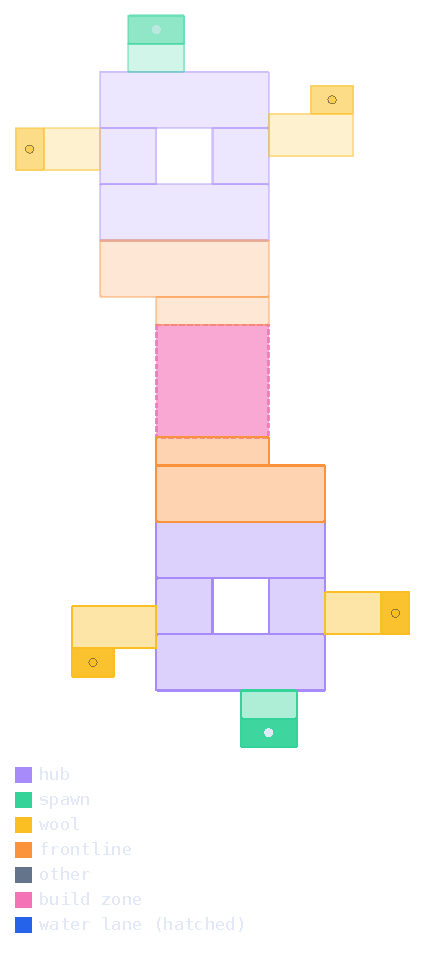
\includegraphics[height=0.52\textheight]{figures/generated/composed-hushwater.pdf}
\end{minipage}%
\hfill
\begin{minipage}[c]{0.60\textwidth}
\small
The board the worked example of \cref{ch:ctw} begins from, drawn by the studio
itself. Eighteen players a side, two teams, \id{rot\_180}, cell 4, seed 5. It
scores 0, meaning no term falls outside its band.

\medskip
Every element of \cref{tab:shares} is visible. The \textbf{hub} is the large violet
body, here in its \emph{ring} form, and the white square inside it is the hole that
\id{CT8} calls the rotation device. The \textbf{spawn} hangs off the hub's far
edge. The two \textbf{wool} approaches, both of the \emph{i} family, stand off its
flanks. The \textbf{frontline} fronts it in orange, in its \emph{single} form. The
pink band across the middle is the \textbf{mid}: the only build zone a composed
board carries.

\medskip
The whole of it is one authored unit repeated through the board's symmetry. Nothing
in the picture is curved, nothing is at a different elevation, and nothing is made
of anything. That is the state a board arrives in, and \cref{ch:ctw} is the account
of what an author does to it next.
\end{minipage}
\caption{A composed board, as \route{GET /api/compose} draws it. The studio renders
this card itself; the figure is its SVG, unedited.}
\label{fig:composed-card}
\end{figure}

\subsection{Boxes: The Units of Allocation}

Allocation deals in \textbf{boxes}: typed bounding envelopes, each carrying a
footprint and a land target. There are five kinds: \id{spawn}, \id{hub},
\id{wools}, \id{frontline} and \id{mid}. A box is an envelope and not a fill
target:
its contents must touch its edges and stay connected, but need not fill it solid.
Boxes exist only during composition and are a model of how an author works rather
than a property of maps.

Two currencies are being spent at once, and the distinction between them is the
mechanism the whole budget rests on. \textbf{Land} is walkable terrain area, set
by the player count. \textbf{Footprint} is total box area, meaning terrain plus
build zone plus gap, and is set by the partition. A build zone costs footprint but
not land.
Converting a terrain piece into a build zone therefore keeps the size and drops
the land, so fragmenting a board conserves footprint and spends land.

\subsection{The Hub as Constraint Source}

The hub is placed first and is the unit's only absolute rectangle; everything else
is positioned against a neighbour. It takes what the budget leaves after the
others have had their share, and never less than a third of it. It is always wider
than deep, the sampled aspect running from 1.3 to 2.4, because a hub grows wider
rather than squarer.

\begin{table}[htbp]
\caption{The budget shares. A spawn is deliberately absent: it is not a share at
all but a box, costing what a room and a run-up cost at the map's corridor width.}
\label{tab:shares}
\small
\begin{tabularx}{\textwidth}{L{3.4cm} r Y}
\toprule
\textbf{Constant} & \textbf{Value} & \textbf{What it means} \\
\midrule
\id{MidShare} & 0.10 & a tenth of \emph{each} unit's land, so the crossing's own
  allowance is a fifth of one team's budget \\
\id{FrontlineShare} & 0.22 & a frontline is the ground the mid is met on, and
  takes about a fifth \\
\id{WoolShare} & 0.12 & each wool about an eighth \\
\id{HubMinShare} & 0.30 & the hub takes what is left, never under a third \\
\id{SpendFloor} / \id{SpendCeiling} & 0.70 / 1.30 & the band the built land must
  land in, or the attempt resamples \\
\bottomrule
\end{tabularx}
\end{table}

Having chosen a size, the hub chooses a \textbf{body}: a ring, a G, a P, a twin, a
double-hole and so on. The body is what publishes, per free run of its edge, the
width that run can carry. Those publications are \textbf{offers},
and an offer's width is a capacity: it bounds the search rather than filtering its
output.

\subsection{Seating and Single-Integer Search}

Each neighbour, whether a wool approach, the spawn or the frontline, arrives as a
request naming a side, a kind, a depth, an along-extent and a rolled family. The
allocator then chooses a \textbf{seat}: a single integer, the offset in the hub's
edge-local coordinates at which the neighbour's along-extent begins. Because the
search runs in one integer, nothing is ever built and then moved.

What a joint records is a \textbf{grant}: the corridor width a consumer was given
across an abutment. An offer is a capacity and a grant is a selection, and
one run can carry two docks at two widths. Keeping those two words apart is load
bearing; an earlier version called both of them the same thing and hid the fact
that they are different quantities.

\subsection{The Crossing}

Between the two fanned halves lies the \textbf{mid band}: the neutral crossing.
Laterally it spans exactly the hull of the opposing front faces and docks flush
against them, so the crossing is one shape with the fronts it connects; in depth
it is the gap. An empty crossing is 30 blocks front to front. A hop, the distance
a player can cross without building, is 12.

Across the gap the composer lays a row of one to three \textbf{stones}. A stone is
shared ground, and that is a property of where it sits rather than of anything it
declares. Their depth follows a grain: a broad-grained row runs 16, 24, 24, 24
blocks up the bands, while a fine-grained one is exactly one corridor wide. Row
counts run one at nano and micro, one or two at milli, and up to three at centi.

\section{Determinism and the Descriptor}

The seed drives every random draw the composer makes, so the same seed under the
same composer version reproduces the same board byte for byte. That is why a
composed board is addressed by a \textbf{descriptor} (players, teams, symmetry,
cell, seed, composer version and schema) rather than by storing its plan. A card
in the browse feed carries its descriptor and its rendered SVG, and pinning one
re-composes the exact plan server-side.

The composer version is part of the identity for a reason worth noting: a card
composed by an older composer reproduces a \emph{different} board from the same
seed. The descriptor records which composer built it, and a stored plan whose
composer has moved on is flagged as stale rather than silently re-composed into
something else.

\section{Refusals of the Browse Feed}

\route{GET /api/compose} scans seeds forward from a cursor, composes each, and
sieves. The structural sieve runs first because classifying a board on its tiny
box masks is cheaper than evaluating it, so a structural reject skips the
evaluator and the render entirely.

Two parameters are refused outright rather than accommodated. A symmetry the
composer does not build for, meaning anything but \id{rot\_180} and
\id{mirror\_z}, answers 400 with an \id{RQ1} finding naming the field. So does a team count other
than two.

\begin{ruling}{Four-Team Boards and the Composer}
The composer builds two-team boards only. That is a limit of the composer as it
stands. It is narrower than the studio's own ceiling of four
(\cref{sec:team-counts}), and narrower again than Capture the Wool, which takes
two or four. A four-team CTW board is authored at the plan tier instead. Until
recently the endpoint read no team parameter at all and answered a two-team board
at 200 for any count asked of it, a request quietly misanswered rather than
refused. It now refuses, on the principle that a board which is not the one asked
for is worse than no board.
\end{ruling}

\section{Wool Asymmetry in Composed Boards}
\label{sec:lopsided}

One property of composed boards is consistent enough to have been measured, and
consequential enough that an adapting agent has to deal with it every time.

On a two-wool board, the two wools are routinely \emph{not} equidistant from the
spawn that has to attack them. Straight-line cell distance from the attacking
spawn to each wool room, measured off boards pinned from the live composer:

\begin{table}[htbp]
\caption{Wool distances from the enemy spawn, off boards pinned from the live
composer. One board in six is balanced.}
\label{tab:lopsided}
\small
\begin{tabular}{l r r r r}
\toprule
\textbf{Request} & \textbf{Seed} & \textbf{wool-a} & \textbf{wool-b} &
\textbf{Worst ratio} \\
\midrule
p20 \id{rot\_180} & 0 & 138 & 94 & \textbf{1.47$\times$} \\
p20 \id{rot\_180} & 1 & 132 & 98 & \textbf{1.35$\times$} \\
p20 \id{rot\_180} & 2 & 142 & 93 & \textbf{1.53$\times$} \\
p30 \id{rot\_180} & 0 & 138 & 99 & \textbf{1.39$\times$} \\
p30 \id{rot\_180} & 3 & 129 & 100 & \textbf{1.29$\times$} \\
p20 \id{rot\_180} & 3 & 127 & 118 & 1.08$\times$ \\
\bottomrule
\end{tabular}
\end{table}

The shape of it is always the same: wool-a is seated deep behind the hub at the
far end of the board, and wool-b is a short spur off the hub's flank near the
front line. One wool is a raid and the other is a walk.

What makes this interesting rather than merely a defect is where the cause turns
out to lie. An agent working through four boards traced it past the wools
themselves:

\begin{quote}
The lopsided wool is caused by where the composer hangs the spawn, and fixing it
moves the spawn.
\end{quote}

The derivation is geometric rather than rule-driven. Equal distance from the
\emph{enemy} spawn forces the two wools to comparable depth. Equal distance from
the team's \emph{own} spawn, given equal depth, then forces symmetry in $x$ about
that spawn's own $x$. A spawn on a flank, which is where the composer puts it on
every board pulled under both symmetries, therefore cannot carry two balanced
wools at all.

That is a good illustration of what adaptation means here. The composer's output
is not wrong; it is under-determined in a way that shows up as a
gameplay asymmetry, and correcting it requires moving a piece the composer
considered settled. An agent that treats the composed plan as fixed inherits the
imbalance.

\chapter{The Rule System and Its Refusals}
\label{ch:refusals}

\section{Two Distinct Rule Sets}

A reader who goes looking for `the rules' will find two collections with
overlapping names, and confusing them makes the system incomprehensible. They
answer different questions.

The first is the \textbf{composer's law}: \LawRuleCount{} identifiers under
\LawFamilyCount{} headings, spanning \LawIdPrefixCount{} id prefixes, held in a
single document that is embedded in the application and parsed rather than
transcribed. It says what a well-formed CTW board \emph{is}: how wide a lane runs,
how far a wool room stands from a spawn, what a build zone may touch. It is
a design document with identifiers attached, and most of its rules are enforced
during composition, where the thing being judged still has a name.

The second is the \textbf{finding catalogue}: \RuleCount{} rules across
\RuleFamilyCount{} families, served live at \route{GET /api/rules}. It is the set of every rule that something,
somewhere, can raise as a complaint about a document. Its scope is the whole
studio rather than the composer, covering sketch geometry, dressing, house styles,
export and the request itself.

The two overlap without either containing the other. The composer's law carries
rules that nothing raises as a finding, and those are deliberately not served: the
question the catalogue exists to answer is \emph{what is this finding}, and a rule
nothing raises has no finding to explain. Measured against the running studio,
\LawServedCount{} of the law's \LawRuleCount{} ids are answered by the catalogue.
Everything else in the catalogue belongs to a gate the composer never touches.

\begin{table}[htbp]
\caption{The finding catalogue by family, generated from the running studio. A
family is the field the API answers with, not the id's prefix: the four
build-zone rules are numbered \id{BZ} and belong to family \id{CT}, so
\RuleIdPrefixCount{} prefixes span \RuleFamilyCount{} families.}
\label{tab:families-live}
\scriptsize
%% Generated from the running pgm-studio API (http://localhost:7894/api) --- do not edit by hand.
%% Source: GET /api/rules

\begin{longtable}{@{}L{16mm}R{12mm}L{112mm}@{}}
\toprule
\textbf{Family} & \textbf{Rules} & \textbf{What it governs} \\
\midrule
\endfirsthead
\toprule
\textbf{Family} & \textbf{Rules} & \textbf{What it governs} \\
\midrule
\endhead
\bottomrule
\endlastfoot
\id{SK} & 28 & The sketch document: shapes, layers, groups and mirroring, and the ground they rasterise into. \\
\id{DR} & 17 & Dressing a built world: where a tree, boulder, building or body of water may rest, and what it may not close off. \\
\id{PL} & 16 & The plan: pieces, placements, walls and the spawns and objectives a board is laid out around. \\
\id{WX} & 13 & The room frame stamped for a spawn or wool: shell, pad, door, iron, and where it stands on its piece. \\
\id{OB} & 12 & Objectives as they are played: where a goal may stand and float, what it is built of, and how the match can end. \\
\id{CT} & 10 & The middle: what the mid is carved into, the holes rotation leaves in it, and the build zones docked there (the BZ-numbered rules). \\
\id{HS} & 10 & House style: the materials and parts a building is authored from, part by part. \\
\id{WL} & 8 & Wool siting: a wool's distance from its spawn, its siblings and the frontline, and the approach into its room. \\
\id{EX} & 6 & The export gate: what must hold before a map document and its world are written. \\
\id{IM} & 6 & World import: the host fetched from, what arrived, and whether it holds a world the studio can read. \\
\id{RL} & 6 & Relief: whether the elevation is the landform the island claims, and whether it can be walked. \\
\id{RQ} & 6 & The request contract: which status a malformed, unknown, conflicting or unreadable request answers with. \\
\id{HJ} & 5 & Wing joints: the ways two rectangles of one building may meet, and the roof that follows. \\
\id{PT} & 5 & Terrain painting: how a theme states its materials, bands and sampled patterns. \\
\id{ST} & 5 & Structure pieces: what a wool-room or spawn piece defines, and the caps on what it may raise. \\
\id{FR} & 4 & The frontline: split or wide, how it docks, and how much of a face a crossing spans. \\
\id{GO} & 4 & Destroy-goal distances, measured by walk: to its own spawn, to the enemy's, and between goals. \\
\id{SP} & 4 & Spawn siting: where a spawn stands on its lane, and what its egress and its door face. \\
\id{DC} & 3 & Destroyables and cores: casing and interior, float against leak, and the material a size is worth. \\
\id{G} & 3 & The board envelope: corridor width, the void gaps a route hops, and map size against player count. \\
\id{HP} & 3 & The footprint a placed building is made of: how many rectangles, how thin, how much ground. \\
\id{ED} & 2 & The edit document: the references it must resolve, and the state it may be applied in. \\
\id{LN} & 2 & Lanes: the corridor width a board is built at, and the run before a junction or a dead end. \\
\id{CO} & 1 & Compose: descriptors that are well-formed and name a board the composer has no shape for. \\
\id{EL} & 1 & Land seams: the step a player cannot walk up, and the palette that steps by it. \\
\id{EZ} & 1 & Editable ground: standable ground nobody can edit, outside the zones a map seals on purpose. \\
\id{PC} & 1 & Piece connectivity: what counts as a join between two pieces, and what does not. \\
\id{SH} & 1 & Shops: the references a shop makes that the document has to define. \\
\midrule
\textbf{Total} & \textbf{183} & \textcolor{ink60}{28 families} \\
\end{longtable}

\end{table}

The full catalogue, rule by rule, is \cref{app:rules}.

\section{Anatomy of a Finding}

Every gate in the studio answers in one shape. A client rendering a refusal never
has to know which gate produced it before it can read one, and this uniformity is
the single most useful property the API has for a machine operator.

A finding is three things: a \textbf{rule id}, a \textbf{sentence}, and
\textbf{what it is about}.

The id is machine-legible and stable forever, so it outlives the task that added
it and never doubles as a task-tracking identifier. The sentence carries the
measured numbers, on an explicit principle. The word \emph{invalid} tells an
author nothing they can fix, so a refusal says \emph{this one is
2\,$\times$\,8} rather than \emph{this one is too small}. What it is about is a \textbf{field} where a
document field can be named, and \textbf{subjects} where the fault indicts things
an editor could highlight. A finding may carry either, both or neither.

One further field matters more to a machine than to a person. A finding states its
\textbf{edit} where the fix is mechanical: a document, a path, an operation and a
value. A reader applies it rather than re-deriving it from the rule's prose. It
is, as the documentation puts it, the half of a finding a model acts on where the
sentence alone is inspected and left.

What a finding deliberately does \emph{not} carry is the rule's classification.
The category and the concerns list are fixed by the id rather than by the raising
site, so they live on the rule and a caller joins them from the catalogue. Putting
them on the finding would put one fact at 96 sites.

\section{Three Severities}

This is the part of the system that has cost authoring runs the most, and it is
the first thing an agent should learn.

\begin{description}[leftmargin=1.6em,style=nextline,itemsep=4pt]
  \item[A refusal] stops the request. The work did not happen. It arrives in the
    error envelope's \id{findings}, and nothing rode along with it.
  \item[A decline] says that a piece of what was posted is \emph{not in what was
    built}. The request succeeded. Something you sent was dropped.
  \item[A complaint] is a remark. The request succeeded and the studio has an
    observation about it.
\end{description}

Both surviving severities ride on a success, under one key:

\begin{quote}
A 2xx JSON object answers \id{warnings} when something was complained about or
declined, and carries no such key when nothing was. \ldots A caller reads
\id{warnings ?? []} and is done.
\end{quote}

The consequence is blunt. A driver that reads only the status code throws away
half of every answer. A board can store at 200 with a floor missing under its
walls, with a theme that painted nothing, with a field it misspelled silently
unread, and the only place any of that is said is \id{warnings}. One run report
names this the dominant failure class in the whole corpus and calls it, exactly, a
200 that isn't a yes.

The distinction between the two is carried on each finding's \id{severity}, and
the documentation is explicit about why it could not be carried anywhere else:
\id{warnings.some(w => w.severity === "decline")} is \emph{something I sent was
dropped}, which no status code and no other field says.

\begin{ruling}{The Findings Read}
\route{GET /map/\{slug\}/findings} is asked on every run beside the others,
because it is the only read that answers \id{SK9}, the gate that knows two shapes
on one layer stacked and the lower one is not in the world. It is a
decline, the channel every other route publishes on keeps complaints alone, and so
a board can store at 200 with a floor missing under its walls and nothing anywhere
says so.
\end{ruling}

\section{The Refusal Envelope and Status Codes}

A refusal on the wire looks like this:

\begin{lstlisting}[language=json]
{ "error": "invalid house style",
  "message": "...",
  "findings": [ { "rule": "HS1", "message": "...",
                  "severity": "refusal", "field": "doorHead.block" } ] }
\end{lstlisting}

\id{error} names the \emph{gate}, such as \emph{objective placement},
\emph{unknown gamemode} or \emph{plan not compilable}, and never the fault itself.
\id{message} is the findings' sentences joined together.

Status codes stay the gate's own, and each means one thing: \textbf{400} a
document wrong as posted, \textbf{404} a subject the route names and the studio
does not have, \textbf{409} well-formed but conflicting with the map's state,
\textbf{422} cannot be processed, \textbf{500} the studio's own fault. Each route
declares which of them it can answer, 95 of 149 operations carrying at least one,
and a test fails if a documented row and its route stop agreeing.

The edge answers in the same shape as the gates. No route under \route{/api}
answers a failure in a shape of its own, and none answers one with no body at all.
A request the framework itself could not bind becomes \id{RQ1} per field under
\emph{request will not read}, naming each field \emph{as the wire spells it}:
\id{region\_id}, not \id{regionId}.

\section{Faults of the Request Itself}

Six rules are about the request rather than the map, and they exist because the
uniform shape held everywhere except at the door. Three are worth knowing by name.

\id{RQ1} is \emph{the document could not be read}: a 400, carrying the field where
the reader knew one.

\id{RQ3} is \emph{a field went unread}, and it is a complaint on a success rather
than a refusal. It is the rule that catches a typo: \id{roof.pich},
\id{wings[1].ptch}. The check walks down the posted value, matching by the name the
\emph{document} uses rather than the name the C\# type uses, and it runs over the
body as posted, before any merge. This is the studio's answer to the failure mode
where an agent posts a field the reader silently drops and believes it took effect.

\id{RQ5} is \emph{the request conflicts with what is stored}: a 409, and the one
refusal where nothing is wrong with the request at all. Every document carries a
revision, a read answers it as an \id{ETag}, and a write may state it back as an
\id{If-Match}. A request with no \id{If-Match} states no precondition and writes.
Protection is opted into by having read first, which is the only way it can mean
anything.

\section{One Question at Four Grains}

The most interesting structural property of the rule system is that the same
question recurs at four resolutions, with a different id at each, and each id can
only see what its own level knows.

Reachability is the worked example.

\begin{table}[htbp]
\caption{One question, \emph{can this be reached?}, asked at four grains. Read
down the column: a board can pass every gate above and still read a third dead.}
\label{tab:one-question}
\small
\begin{tabularx}{\textwidth}{l L{3.6cm} Y}
\toprule
\textbf{Rule} & \textbf{Grain} & \textbf{The question it asks} \\
\midrule
\id{WX6} & one piece of the plan & can a door be cut into this room at all \\
\id{PL9} & the whole plan & can a capturing team's spawn reach this wool \\
\id{EX1} & the built world & is the ground the rasterizer produced connected \\
\id{DR-PASS} & one building & does this building leave eight blocks to get past it \\
\id{DR-SLOPE} & one footprint & is this building's footprint level enough \\
(none) & a measurement & is reachable ground ground any journey actually uses \\
\bottomrule
\end{tabularx}
\end{table}

The documentation draws the conclusion, and it is the best argument in the system
for why there are four documents rather than one:

\begin{quote}
A finer grain exists only because a coarser one does \ldots Collapsing the four
documents into one would not simplify the rules. It would remove the vocabulary
each rule uses to say precisely what is wrong.
\end{quote}

Ids are grouped by what they are \emph{about}, never by which gate happens to ask.
The same objective rule is asked at the compile gate against a plan's pieces and
at the export gate against the ground the rasterizer produced, and a rule that
changed its name between the two would be two rules.

\section{Bands and Targets}

\Cref{ch:division} stated this as a finding; here is the mechanism. Rules divide
by \emph{kind}, and the two kinds most often confused are the target and the band.

A \textbf{target} is prescriptive and per-request: this compose wants exactly two
frontline runs, connected. A \textbf{band} is descriptive and measured off the
corpus: authored maps run one to seven frontline runs. The distinction is load
bearing, and the documentation states the failure precisely. A band pressed into
service as a target silently turns an observation about the corpus into a
requirement on the generator.

Several rules therefore read authored bands whose values depend on what the board
is played for. A frontline width cap of six to eight cells is the wool board's
figure; on a board played for cores or destroyables there is no width cap at all,
because a wide front feeds a wool lane and a destroy board has none. One run put
it as the most transferable thing it learned: three boards of experience on one
objective family taught it nothing about the next.

This is why \route{GET /api/rules/terms} exists. A driver asks what band is
enforced on \emph{this} board rather than writing down a number that was true of
the last one. The \ScoredTermCount{} scored terms and their bands are \cref{app:terms}.

\section{Nine Representative Rules}

The law is large and mostly technical, but a handful of its rules carry most of
what a reader needs to know about what the studio thinks a map is. These are
quoted as the law states them.

\paragraph{The corridor ladder.} \id{G2} fixes the whole board's scale:
the map's corridor width is the size band's, stated in blocks (12 at nano, 14 at
micro, 16 at milli and centi), with the wool approach one rung under it.
Measured over 359 built CTW maps.

\paragraph{The jump, not the bridge.} \id{WL12} is the newest wool rule and the
one an adapting agent breaks most often:

\begin{quote}
A bay or a hole beside a goal is at least 16 blocks across. Negative space is
crossed by \textbf{jumping} long before it is crossed by building \ldots Stated in
\textbf{blocks}, never in cells: a floor stated as a cell count moves with the
grid scale, and a jump does not care what the grid was.
\end{quote}

The floor is 16 blocks where the space touches a wool room or spawn and 12 where
it touches neither, because a hole in a team's own ground is crossed on purpose.

\paragraph{Holes are the rotation device.} \id{CT8} is the clearest statement in
the law of a rule that exists for a gameplay reason rather than a geometric one.
The closure encloses internal void pockets in every seed measured, and the
author's reason is that a loop around a hole gives alternative routes between
lanes without retreating through a single chokepoint. It is not mandatory, since
not every map has to have one though most do, so a holeless plan is flagged and
never blocked.

\paragraph{The strait.} \id{CT12}: on a two-team wool board the direct crossing
between the two team islands spans 15 to 40 blocks. Closer is two halves all but
merged; farther is a crossing nobody bridges.

\paragraph{The unwalkable seam.} \id{EL1}: a land seam of two blocks or more is
ground a player cannot walk up. The consequence is what the rule is for. On a
board built from the authored height palette every non-flush seam is a step nobody
walks, so the seam wants a ramp or a flight carved into it, and the check's output
is the work list for that pass rather than a fault to redraw around.

\paragraph{The mid never touches a wool.} \id{BZ6}, short and absolute: otherwise
players bridge freely through the mid straight into the point and there is no
gameplay direction.

\paragraph{A zone is bounded by the ground it docks.} \id{BZ9} forbids the
\emph{overhang}: a stretch carried beyond the last ground it meets, which connects
nothing and reads as no man's land a player walks into and stops.

\paragraph{The defence triangle.} \id{WL10} bans a specific failure: a front-near
wool whose spawn is far, beside a back wool whose spawn is adjacent, so that the
defender always guards the wrong door.

\paragraph{The destroy goal's ratio.} \id{GO1}: a destroy goal sits three to four
times as far from the enemy's spawn as from its own, measured by the walk over the
surface. Under the band the goal falls to a rush before a defence can form; over
it the attack is a march across the whole board into a set defence.

\begin{ruling}{Distance Is Measured as a Walk}
A distance between two things on a board is the walk between them over the
walkable surface. It is eight-connected, a diagonal costs what a player walks
rather than two steps, a climb is charged the blocks it takes to place, a fall is
counted but not charged, and the route goes around voids. Never the straight line through the air. Every
distance in every rule is this.
\end{ruling}

\chapter{Ground: Outlines and Their Construction}
\label{ch:ground}

\section{Islands and the Height Convention}

The ground level deals in \textbf{shapes} on \textbf{layers}, grouped into
\textbf{groups}. A shape has an outline, a floor and a thickness, and where its
ground touches or overlaps another shape's in the same group, the two build one
\textbf{island}.

The first thing to get right is the height convention, because it is off by one
from the obvious reading and an agent gets it wrong every time otherwise:
\id{base\_height: 9} puts the top block at $y=8$, not $y=9$. A column read at such
a shape answers grass at $y8$, dirt at $y7$ and $y6$, stone from $y5$ to $y1$, and
bedrock at $y0$.

\section{Four Forms of Outline}

\subsection{Polygons and the Rectangle}

A polygon is a ring of points. A rectangle is not: it states bounds rather than
points, and so it is restated as a four-point polygon before any point of it can
move. That restatement is invisible in the document and load-bearing in practice.

Three routes edit one point without disturbing any other:

\begin{lstlisting}
PATCH  /api/map/{slug}/sketch/shapes/{id}/vertices/{index}   {x, z}
POST   /api/map/{slug}/sketch/shapes/{id}/vertices           {after, x, z}
DELETE /api/map/{slug}/sketch/shapes/{id}/vertices/{index}
\end{lstlisting}

The insert has index arithmetic that bites. A point added \id{after: 0} lands at
index 1, and every later index goes up by one, so a pair of points previously at
2 and 3 migrates to 3 and 4. An agent replaying a list of edits by index, computed
against the original ring, will scramble the outline.

\subsection{Height as a Per-Vertex Field}

\id{anchor\_heights} is one thickness per vertex, in the same ring order, and the
surface between them is interpolated across the face. A six-point island carrying
\id{[9, 12, 16, 17, 17, 14]} is the plane $9 + x/4 + z/4$ in the island's own
frame. That is a tilt, authored with six numbers.

\subsection{Curves and B\'ezier Handles}

Four ways to state an outline that is not made of straight edges. A \textbf{circle}
takes a centre and a radius and the studio draws it as a 64-sided polygon. A
\textbf{lasso} is, in the document, simply a polygon. The difference is the
canvas, which traces it freehand and simplifies the trace at a four-block
tolerance. And any polygon edge can be bowed with Bézier handles.

The Bézier contract is worth stating exactly, because every part of it is a place
to go wrong:

\begin{quote}
\id{controls} is keyed by a vertex's index as a string, and every handle is an
\textbf{absolute point on the board}. The edge from vertex $i$ to vertex $i+1$ is a
cubic curve from vertex $i$, pulled by \id{controls[i].out} and
\id{controls[i+1].in}, to vertex $i+1$. So a vertex's \id{out} bends the edge after
it, and its \id{in} bends the edge before it. The studio samples every curved edge
16 times, and the curve still passes through every vertex.
\end{quote}

Bowing one edge is two handles:

\begin{lstlisting}[language=json]
"controls": { "0": { "out": [74.67, -6] }, "1": { "in": [81.33, -6] } }
\end{lstlisting}

Rounding a whole ring is a closed-form recipe rather than a hand fit: at each
vertex $P$ with neighbours $\mathit{previous}$ and $\mathit{next}$,
\[
\mathit{in} = P - \frac{\mathit{next} - \mathit{previous}}{6}, \qquad
\mathit{out} = P + \frac{\mathit{next} - \mathit{previous}}{6}.
\]

\begin{ruling}{Limits on a B\'ezier Handle}
Keep each handle at least as far \emph{along} its edge as it is \emph{away} from
it, and keep the bulge under about a third of the edge's length. Past that the
curve crosses itself.
\end{ruling}

\subsection{Polylines}

A polyline is a line with a width: its points are a centreline, and the band
\id{radius} blocks to each side of it is ground. The order of operations is the
fact to know:

\begin{quote}
The points are \textbf{smoothed first}, by a centripetal Catmull--Rom spline with
eight samples between each pair, and only then offset \id{radius} blocks to either
side, so four points draw a curve rather than three chords. The ends are cut
square.
\end{quote}

\begin{lstlisting}[language=json]
{"id":"line-solid","type":"polyline","operation":"add","floor":0,
 "base_height":9,"vertices":[[0,10],[13,3],[27,17],[40,10]],
 "radius":3,"stroke_edge":"solid","stroke_seed":7}
\end{lstlisting}

\id{stroke\_edge} takes three values with numbers attached. \id{solid} keeps one
width. \id{rough} lets it swing up to 45\% either way with the two sides wandering
apart, seeded by \id{stroke\_seed}. \id{tapered} narrows it to 35\% at the ends.
A polyline also takes \id{anchor\_heights}, which are heights at its points, with
every block taking the height of the nearest place along the line. A lane can
therefore rise.

Two facts separate a polyline from things that look like it. A polyline whose ends
lie \emph{inside} two islands joins them into one, which is how a land bridge is
drawn. And, in the distinction that costs an afternoon, a polyline shape \emph{is
ground}, whereas the \id{stroke} prop, which looks alike, repaints the top course
of what it crosses and adds no ground at all.

\begin{ruling}{Self-Overlap in a Polyline}
The band is one outline filled even--odd, so where its two sides cross they cancel
and build void. The studio names it \id{SK25}. Four points across 26 blocks at
radius 3 lap in every bend; the same four points spread over 40 blocks clear. A
coil is drawn as one polyline per part-turn.
\end{ruling}

\section{Overlap: Height and Paint}

Where two shapes cover a cell, two questions are settled separately, and conflating
them is a common error.

\begin{quote}
The height and the paint of an overlap are decided separately. Where two shapes
cover a cell, the taller one gives the column its height, and the paint goes to the
\textbf{smallest themed shape whose top is that tallest top}.
\end{quote}

So on a flat island where a yard and a meadow both stand at 9, the yard being
smaller means the overlap paints as the yard. A lawn smaller again paints as the
lawn inside the yard. Height is decided by tallest; paint, among the shapes that
tie for tallest, by smallest.

\begin{ruling}{Occlusion Within a Layer}
On one layer the taller shape takes the whole column, so a lower shape drawn inside
a higher one simply is not there, and the studio names it \id{SK9}. A sunken place
inside a raised one is drawn as shapes \emph{around} it, or on a layer of its own. This is the same rule \cref{ch:layers} states from the other side.
\end{ruling}

\section{Faces and Band Stacks}

Where a shape's ground drops, whether over lower ground or over the void, the
exposed side is a \textbf{face}, and a theme can stripe it with a band stack.

One property of that stack is not what it looks like:

\begin{quote}
A band stack does not cycle: past its last band, \id{"ending": "repeat"} hands
every further course to that last band.
\end{quote}

So striping a face sixteen courses tall with a four-course pattern means writing
the four courses out four times. A stack that reads as four bands in the author's
head is twelve bands in the document.

The other property is that only the courses standing \emph{above} the neighbouring
ground are face. The same yard, stepped up from a meadow on one side and dropping
to the void on the other, reads four striped courses on the first and the whole
stripe from top to bedrock on the second.

\section{Five Forms of Ascent}

Getting from one height to another is its own small craft, and the studio offers
five forms: a ramp (one polygon with anchors at each end), a stair (one polygon
with deeper treads), a turned flight (two polygons with a landing between), a run
of steps (one rectangle per tread), and a floating flight (one raised slab per
tread, with air under each).

One rule governs all of them and it is the most counter-intuitive fact in the whole
ground model:

\begin{quote}
\id{anchor\_heights} are heights at a polygon's corners, and every block reads the
slope at its own centre and rounds. A flight therefore comes out even \textbf{only
when the anchors sit half a riser past its first and last tread}: a 2-deep stair
whose treads are 1 to 7 states 0.5 and 7.5. Whole-number anchors 8 and 1 over 16
blocks build treads 1, 2 and 3 deep. The ramp works with whole numbers because one
block up per block rounds cleanly.
\end{quote}

And a consequence that decides how a flight can be authored at all: the studio's
canvas rounds anchor heights to whole blocks, so the half-block form can only be
written into the document. Drawing an even stair by hand means one rectangle per
tread instead.

\chapter{Relief: The Shaping of Ground}
\label{ch:relief}

\section{Relief as a Solve}

Relief is how flat ground becomes terrain. It is stated per group, and it is a
\emph{solve}: the studio takes a small number of statements about where the ground
must be, and computes a height for every cell in between.

The single most important property follows from that:

\begin{quote}
A relief replaces the top of every column it solves, and the heights it solves come
from its marks and pushes. A solved shape's own \id{base\_height} therefore decides
nothing about where the ground ends up.
\end{quote}

The technique cards prove this rather than assert it. The same relief is applied to
two plots whose shapes are drawn at different heights, 13 and 9 in one and both 9
in the other, and the built ground is identical: 2304 columns compared, 0 differ. An author who tunes a shape's drawn height to influence a solved surface is
tuning a number nothing reads.

\section{Constituents of a Relief}

\begin{lstlisting}[language=json]
"relief": { "stepped": {
  "base": 11, "reach": 0, "step": 1,
  "marks": [
    { "id": "upland-bench", "kind": "area", "h": 13, "bevel": 2,
      "ring": [[-28,-26],[-20,-30],[-8,-29],[-3,-22],
               [-4,-12],[-10,-7],[-22,-8],[-28,-14]] },
    { "id": "lowland-bench", "kind": "area", "h": 9, "bevel": 2,
      "ring": [[-46,8],[-38,5],[-20,6],[-6,5],
               [-2,10],[-8,15],[-26,14],[-44,15]] } ],
  "pushes": [
    { "id": "knoll", "amount": 1, "falloff": 3, "crown": 3.5,
      "roughness": 0, "seed": 1,
      "ring": [[-32,-32],[-21,-32],[-18,-25],[-22,-18],[-32,-19]] } ] } }
\end{lstlisting}

A \textbf{mark} pins ground. An \id{area} mark holds the middle of a region at a
stated height, and its \id{bevel} softens the edge. A \textbf{push} raises a region
by an amount over a falloff, with a crown and an optional roughness.

\Cref{tab:marks} is the full set. A mark is placed rather than sampled, for the
same reason a prop is: a decision about where the high ground is decides how the map
plays, so it belongs to the person making it rather than to a noise field.

\begin{table}[htbp]
\caption{The five marks. Each pins part of the footprint at a chosen height; the
solve fills between them.}
\label{tab:marks}
\small
\begin{tabularx}{\textwidth}{L{1.7cm} L{5.2cm} Y}
\toprule
\textbf{Mark} & \textbf{Pins} & \textbf{Says} \\
\midrule
\id{point} & a disc of a given radius & a summit, a hollow, a spot height \\
\id{line} & a band reaching \id{r} either side of a polyline, optionally with
  several heights along its run and a tread held flat &
  a ridge, a valley floor, a shoulder falling as it runs, a road switching back
  down a hill \\
\id{area} & every cell inside a ring, at one height or one per vertex, with an
  optional graded bevel inside its edge &
  a bench, a mesa top, a sunken floor, a shelf cut into a hillside \\
\id{rim} & the footprint's own outer rings & where the land meets the void \\
\id{scarp} & a band either side of a drawn line, at two heights, with the face
  between them left free &
  a break of slope, and the mark that decides where players can go \\
\bottomrule
\end{tabularx}
\end{table}

A line mark's \id{r} reaches either side of the centreline, so the band it writes is
\emph{twice} it: a stated 6 holds a twelve-block strip. The rim is optional, and it
is what keeps a hill inside its shape. Without one, marks alone decide the whole
surface, so a shape carrying a single high mark rises to that height everywhere and
runs off its own edge.

The most useful sentence about marks is about the space \emph{between} them:

\begin{quote}
Each \id{area} mark holds the middle of one meadow at its own height, and its
\id{bevel} softens the edge. The ground between the two benches is pinned by
nothing, so the solve grades it. \textbf{That free band is the connection.}
\end{quote}

Relief is therefore authored by pinning as little as possible. Pin the two things
that must be at particular heights and let the solve invent the slope between them;
pin everything and there is no slope, only a set of plateaux.

\begin{ruling}{Agreement of a Push's Gradients}
A push publishes two gradients: its skirt, which is \id{amount / falloff}, and its
crown. A knoll reading 0.33 up its skirt and 0.31 to its crown is smooth. Where the
two disagree the push steps at its own outline instead of rising into the ground,
and the studio raises \id{RL6}.
\end{ruling}

\section{Relief Scope: Three Treatments}

The question is what a relief does to a shape that already has a height. There are
three answers and the difference between two of them is the difference between a
join and a cliff.

\begin{description}[leftmargin=1.6em,style=nextline,itemsep=5pt]
  \item[No scope at all. The shape joins the solve.] Its drawn height is
    discarded and the relief decides where its ground goes. This is the default and
    it is right for terrain.
  \item[\id{hold}. The shape keeps its height and is still arrived at.] Its cells
    stay in the solve but are pinned at the height the shape states, so the ground
    around it is solved \emph{knowing where it has to arrive}.
  \item[\id{exclude}. The shape is a hole in the solve.] The relief bends round
    its edge exactly as it bends round the void, and nothing climbs to meet it. The
    shape keeps its faces.
\end{description}

\begin{figure}[htbp]
\centering

\includegraphics[width=\textwidth]{techniques/relief-on-shapes.png}

\medskip
{\small\begin{minipage}{0.95\textwidth}
The same three shapes, built three times under three treatments, sixty-four blocks
apart in one world. Each is a raised works yard, an upland meadow beside it and a
lowland below both. \textbf{Left}, the relief smooths the two meadows into one slope
and runs up against the yard without moving it. \textbf{Centre}, both meadows are
drawn at one height and the same relief builds it alike, block for block.
\textbf{Right}, the upland is held at the height it was drawn at and the relief is
spent only on the grade from the lowland up to it.
\end{minipage}}
\caption{The three treatments, side by side rather than in three folders. The
comparison is controlled: the shapes differ only in the heights they are drawn at
and in what each states about its scope.}
\label{fig:relief-scope}
\end{figure}

The distinction between the last two is measurable, and the technique card measures
it. Along one line, a shape drawn at 12 dropping to ground drawn at 8:

\begin{table}[htbp]
\caption{The same shape under \id{hold} and under \id{exclude}, read along one
line. \id{hold} makes the join; \id{exclude} leaves a face.}
\label{tab:hold-exclude}
\small
\begin{tabular}{l r r r r r r r r r}
\toprule
$z$ & $\cdots-1$ & 0 & 1 & 2 & 3 & 4 & 5 & 6 & 7 \\
\midrule
as drawn                        & 12 & 8 & 8 & 8 & 8 & 8 & 8 & 8 & 8 \\
\id{hold}, with the relief      & 12 & 12 & 11 & 11 & 10 & 10 & 9 & 9 & 8 \\
\id{exclude} instead            & 12 & 8 & 8 & 8 & 8 & 8 & 8 & 8 & 8 \\
\bottomrule
\end{tabular}
\end{table}

\begin{quote}
\id{exclude} on the upland would not make the join. An excluded shape is a
\textbf{hole in the solve}, the relief bends round its edge as it bends round the
void, and nothing climbs to meet it.
\end{quote}

The corresponding failure runs the other way. A built thing, such as a yard, a
plinth or a platform, wants \id{exclude}, because it should keep its faces. The same
layout built without it puts the yard's top at 11 instead of 17: the relief simply
replaced the height it was drawn at.

\section{Joins Between Grounds}

This is the craft rule the whole chapter exists to support, and it is stated in the
authoring discipline rather than in the API.

A board is two or three or four \emph{grounds}, each stated by the one instrument
that can state it, and every join between them is chosen rather than left over.
A beach and the dunes behind it are two reliefs on two layers, held at different
heights, because relief solves per layer and the fields are shifted into world $Y$
separately, so two reliefs can meet. One relief across both is one field, and
there is no join at all.

That is the difference between a board that reads as a place and a board that
reads as one field with a gradient in it.

\begin{table}[htbp]
\caption{A shore board, worked through: each ground stated by the instrument that
can state it, and each join chosen.}
\label{tab:shore}
\small
\begin{tabularx}{\textwidth}{L{3.1cm} L{4.1cm} Y}
\toprule
\textbf{The ground} & \textbf{Stated by} & \textbf{Why that instrument} \\
\midrule
the beach & a relief with flow: marks pinning only the waterline, a grain, a low
  step & it has to read as deposited, so nothing is pinned that does not have to be \\
the dunes behind it & a second relief, on its own layer, held a little higher &
  two reliefs can meet; one relief across both is one field and no join \\
the yard the houses stand on & a shape carrying \id{relief\_scope: "exclude"} &
  the footprint leaves the solve, so the two tiers meet at a \emph{face} \\
beach $\rightarrow$ dune & the two reliefs' own meeting, across the layer seam &
  the join has a shape because two fields made it \\
dune $\rightarrow$ yard & an authored flight: \id{height\_mode: "level"},
  anchors, \id{skirt: 0}, a material rather than a theme, run at least twice the
  rise & a relief graded across the seam deletes the boundary; a flight states it \\
\bottomrule
\end{tabularx}
\end{table}

\begin{ruling}{One Map, Several Grounds}
Plains everywhere is not simplicity. It is one instrument.
\end{ruling}

\section{Shapes Laid on Solved Ground}

Sand on the beach, gravel on the tide line: something that paints rather than
shapes. Such a shape carries a theme, a \id{base\_height} equal to the ground it
lies on, and, in the part that goes wrong, \textbf{no} \id{relief\_scope} at all.

Two reasons. A shape owns the paint only on a cell it forms the surface of, so one
stated lower runs under the ground, paints nothing, and says so on a 200. And a
\id{relief\_scope} is a statement about \emph{height}: \id{follow} seats the shape
on the solved field and then pins its whole ring there rigidly, which over a
terrain patch is a floor. The strand solves level to the block, and every mark
inside it is overwritten in silence.

\section{The Relief Read}

One call answers what the marks did to \emph{each other}, which no render can
show. It is
\route{POST /api/map/\{slug\}/sketch/relief/read}, given the stored layout.

It answers, per group: the cell count, the low and high, the relief, walk and
scramble tiers, the faces, the cliffs, and four fields that are the reason to ask
it at all.

\begin{description}[leftmargin=1.6em,style=nextline,itemsep=4pt]
  \item[\id{silentMarks}] every mark that landed nowhere. A mark that pinned nothing
    is invisible in every picture.
  \item[\id{seams}] the pairs that meet on a step. A seam naming a \emph{shape}
    rather than a mark is a \id{relief\_scope} pinning ground the marks were meant
    to shape.
  \item[\id{level} and \id{largestField}] the two numbers that say whether the
    ground has a shape at all. Over about 0.45 and 0.13 respectively, it is a table
    with edges.
  \item[\id{landform}] what the solve thinks it made: \emph{rolling},
    \emph{plain}, and so on.
\end{description}

\begin{ruling}{Relief and Symmetry Folding}
Any symmetry mode folds the relief across the centre, a group's \id{mirrors: false}
does not change that, and a layout stating no \id{mirror\_mode} takes
\id{rot\_180}. A board meant to solve unfolded has to say \id{mirror\_mode: "none"}.
\end{ruling}

\section{The Limits of Relief}

The repository's author states the danger directly: relief should be used, and
solid structural areas matter. A board whose every square is rolling has no ground
a fight can happen on, and an agent reaching for relief to make a board interesting
will reliably overdo it.

The counterpart discipline is a count. Run over a finished spec: how many reliefs,
how many marks and of what kinds, how many pushes, how many shapes at each height
mode, how much made ground, how many polylines, how many made layers, how many
copied trees. A zero in that list is not a fault. Four zeros is a board that used
one instrument and called it terrain.

\chapter{Layers and Literal Depth}
\label{ch:layers}

\section{One Span per Column}

A sketch layer is a slab, and the one sentence that governs it is this:

\begin{quote}
A layer holds exactly one span per column, and where two adds contest a cell
\textbf{the taller replaces the shorter outright, floor included}.
\end{quote}

Those last five words are, as the repository's own account of the technique puts
it, the whole of what makes sculpture possible. They mean that a stack of nested
shapes writes an arbitrary height field with no subtraction anywhere and no
per-column authoring. Draw a wide low disc, then a narrower taller one on top of
it, then a narrower taller one again, and the result is a stepped mound. Nothing
computed a mound; at every column the tallest add present is simply the one that
survives.

It also means the word \emph{slab} is misleading:

\begin{quote}
A layer is not a flat slab. It is one arbitrary \emph{height field}, a
\id{(floor, top)} pair per column, and a stack of layers is a set of those fields
with air between them. Any solid whatever can be written in that form.
\end{quote}

\subsection{The Algebra of a Single Layer}

Within a layer, a group of shapes resolves as
\[
\bigl((\text{adds} - \text{subtracts}) \cup \text{override-adds}\bigr) - \text{override-subtracts}.
\]

Two consequences follow, and both catch authors out. An \emph{ordinary} add loses
to a subtract over the same column regardless of which was authored first, because
the subtract side of the algebra runs before either shape's override flag is
looked at. And the two add sets each settle among themselves by height before the
override plane overwrites the ordinary one, so an override add replaces the column
it lands on whatever its height is. That is what puts a one-block floor
inside a twelve-block wall, and a threshold through a doorway, with neither shape
cut against the other.

\begin{ruling}{The Limit of Nesting}
A bowl falls inward, and the outer disc that should keep only its own ring is also
the tallest thing over the middle, so nested discs come out as a flat plate. A
falling field needs shapes that do not overlap at all.
\end{ruling}

\section{A Storey as Rock with Holes}

This is the part that most often has to be unlearned. The instinct, drawing a
second storey under a map, is to draw the rooms. That produces nothing, and the
reason is the one-span-per-column rule:

\begin{quote}
A sketch layer carries one span per column, so a room drawn on its own leaves every
other column of that storey empty. The board's lower half is air and the ground
above it floats. What is stated is the \textbf{rock}, over every column the board
has, and the rooms are the holes in it.
\end{quote}

Building an undercroft therefore takes three coordinated moves.

\subsection{The Lift}

The ground has to be raised to make room underneath it. That means the plan states
a higher surface, \id{"globals": \{ "surface": 22 \}}, and the finish thins the
slab to its top courses, leaving the rest free.

Moving only one of the two fails in a way that is confusing to diagnose. If the
surface is lifted without telling the plan, the spawns stay at their old height
while the ground goes up, and the buildability check then reports every placement
as standing over open void, because the marker is a dozen courses under the ground
it names.

\subsection{The Layer Below}

\begin{lstlisting}[language=json]
{ "id": "under", "name": "Undercroft", "base_y": 0, "below": true,
  "shapes": [
    { "id": "rk1",  "type": "rectangle", "operation": "add",
      "floor": 0, "base_height": 14, "theme": "rock",
      "min_x": -50, "min_z": -50, "max_x":  50, "max_z": -30 },
    { "id": "rk2",  "...": "min_x -50, min_z -30, max_x -30, max_z 30" },
    { "id": "rk3",  "...": "min_x  30, min_z -30, max_x  50, max_z 30" },
    { "id": "rk4",  "...": "min_x -50, min_z  30, max_x  50, max_z 50" },
    { "id": "hall", "type": "rectangle", "operation": "add",
      "floor": 0, "base_height": 8, "theme": "room",
      "min_x": -30, "min_z": -30, "max_x": 30, "max_z": 30 }
  ],
  "groups": [ { "id": "under", "mirrors": false, "shapeIds": [ "..." ] } ] }
\end{lstlisting}

\id{below: true} inserts the layer under the compiled ground rather than over it.
Every shape in it is an \textbf{add}: the rock is banded round its hole rather
than cut with a subtract. Four rectangles ring the hall; the hall is a fifth.

The depth arithmetic is then by construction rather than by any field. The rock
runs from floor 0 for fourteen courses, meeting the landmass's underside at
$y=14$. The hall is a shorter span in the same columns, floor 0 and eight courses,
so its floor is stood on at $y=7$ and it has six courses of headroom under the
rock's ceiling. Stated generally: a storey's headroom is the gap between two spans
and needs no field at all.

\subsection{Stamping Without Mirroring}

The group carries \id{mirrors: false}, and that is not a detail.

\begin{quote}
The storey covers the whole board, so its own \id{rot\_180} image lies over it;
fanning it would put every column's ground back twice. A layer that covers only one
half is fanned and one that covers both is stamped once.
\end{quote}

The cost of stamping once is that the layer then has to be its own image, which is
to say symmetric by construction rather than by machinery.

\section{Three Failure Modes}

\subsection{Subtracts Across Layers}

The natural way to make a hall is to cut it out of a slab. The studio refuses
that, twice:

\begin{lstlisting}
POST /map/from-documents   422
SK13  's0' fills 3600 column(s) that 'cut1' takes away -- from (-30, -30)
      -- 's0' is on layer 'ground' and the subtract on 'under', and a
      subtract reaches only the layer it is on
SK13  'descent' fills 56 column(s) that 'cut1' takes away -- from (-22, 2)
\end{lstlisting}

The reason is semantic rather than technical. A subtract states that the column is
\emph{empty}, and the landmass over it then fills what the storey below said was
void. So the recipe is banding: split into bands at every hole edge along one
axis, split each band along the other, and drop the parts that fall inside a hole.

The sculptor's version of the same move avoids the problem at the outline level:
an outline is filled even--odd, so a ring is drawn as the outer ellipse, slit
inward, the inner ellipse the other way round, and closed: one polygon, no
subtract, no refusal.

\subsection{Silent Occlusion}

This is the failure to be most afraid of, because everything reports success:

\begin{quote}
Writing the rock as one rectangle over the whole board and the hall as a shorter
add in the same columns compiles, builds and exports with the gate \textbf{open},
and there is no hall.
\end{quote}

No gate fires, and the studio is right not to fire one: two adds at one floor are
ordinary ground, and the taller winning is exactly what \emph{height is the tallest
add} means. That is precisely why the banding is the technique rather than a detail
of it.

\subsection{Verification by Count}

A missing column in a storey is invisible in every render, because the rock above
and below it hides the gap. So it is not inspected; it is counted. The undercroft
showcase states its check as a number: over the board's 10,000 columns, none is
bare and none carries two spans.

The honest cost of the technique shows up when the holes get complicated. A hall is
four bands. A maze of a hundred corridors and links leaves \textbf{213 rock bands}
between them.

\begin{ruling}{Banding Versus Overlay}
The rock is banded round the hall because the two differ in \emph{height},
fourteen courses against eight, and on one layer the taller add wins the column
outright. A basin and a hall that are the same eight courses in the same columns
win nothing from each other: the geometry is identical either way and only the
paint differs. Getting it the wrong way round is silent in both directions: a
banded-out basin is the same world, and a shorter add inside a taller one is no
room at all.
\end{ruling}

\section{Override and Floor}

An underpass makes the mechanism measurable. A deck and a cut occupy the same
cells. Without \id{override}, a column read at the deck answers \emph{0 solid
blocks, void}: the ordinary add lost to the subtract.

With \id{override: true} but no \id{floor}, the studio refuses:

\begin{lstlisting}
POST /map/from-documents   422
[refusal] SK13  'deck' fills 260 column(s) that 'gullet-cut' takes away
                -- from (-28, -5)
\end{lstlisting}

The reason is that \id{floor} defaults to zero, the very bottom of the shape's
column, so an override add with no stated floor spans from the world's floor to
its own top, and once again fills what the subtract declared void.

\id{floor} is the field that decides, and it decides by setting where the column's
own span \emph{starts}, not by any relation to the ground it replaces. With
\id{"floor": 13, "base\_height": 4} the same column reads four blocks, $y13$ to
$y16$, and nothing recorded beneath. The rule that separates a lid from a fill is
then exact: an override add resting \emph{above} the subtract's floor moves that
span up and records nothing beneath it, and the gate is silent on it; the same
shape at the subtract's own floor is the refusal above. The difference between the
two documents is one field.

\subsection{The Scope of the Constraint}

It is often said that the studio has no floor underneath a shape. That is not
quite it, and the accurate version is more useful:

\begin{quote}
A column carries one span \emph{per sketch layer}, not one span. \ldots So the
honest statement is narrower and more useful: \textbf{one layer cannot stack, and
stacking is what layers are for.}
\end{quote}

\subsection{The Stairwell}

The two mechanisms combine in the move that connects a storey to the one above it:

\begin{lstlisting}[language=json]
{ "id": "descent", "type": "polygon", "operation": "add",
  "override": true, "keepClear": true,
  "floor": 8, "base_height": 14, "theme": "stair",
  "height_mode": "level", "skirt": 0,
  "vertices":       [[-22,2],[-18,2],[-18,16],[-22,16]],
  "anchor_heights": [   1,     1,      14,      14   ] }
\end{lstlisting}

Two numbers matter and they are the same number. The flight's \id{floor} is 8,
the hall floor's own top, so it rests on the storey below rather than driving
through it. And an override add is what cuts the shaft; a subtract there would be
the refusal above again.

One rasterizer fact is worth carrying away from this, because it explains a class
of ugly output that looks like a bug. A ramp at one course per cell only rasterizes
cleanly because the surface is sampled at the cell's centre and \emph{floored} into
the column. Rounding to nearest instead puts every sample of a 1:1 grade exactly on
the boundary, and the flight comes out as a beat of noughts and twos.

\section{Paint Order in a Stack}

Layers are written bottom-up and the painter walks them in document order, which
produces one failure worth stating plainly: a storey listed after one that stands
over it finds no stone left to paint. An undercroft goes \emph{before} the compiled
ground in the document, and \id{below} is what puts it there.

Two further properties of a stacked board catch authors out. A plain layer's paint
bands run from the bedrock course whatever its \id{base\_y}, since only a layer
marked as a \emph{made} thing is painted over its own span, so every ground theme
on such a board wants a fill that is not trivial. And a placement names its storey
explicitly; naming none takes the top surface, which on a roofed goal is the roof.

\section{Made Layers}

A layer marked \id{kind: "made"} is out of the stacking rules: it is painted over
its own span, and it is exempted from the walk that checks a board's pairs and the
walk that checks its reachability. The reason is stated as a fact about the shape
rather than as a convenience. A solid standing in a hill has no gap to lose, and
its roof is not a stair somebody forgot.

A made layer also carries \id{part\_of}, naming the thing a run of layers is sliced
from, and may carry \id{seat: "ground"}, which settles the run onto the terrain
together rather than each slice finding its own height. That is how a sculpted
landmark, whether a dome, a spire, a tapered tower or a gatehouse, is authored: as
ordinary sketch shapes, circles and polygons with a floor and a height, rather than
as stamped block soup.

\chapter{Terrain: Themes, Materials and the Slope Axis}
\label{ch:terrain}

\section{A Second Pass over a Finished World}

Painting terrain is not part of building it. It is a second pass over the realized
world, run after every structure has been stamped, and it adds no geometry at all.
It reads the terrain the world builder placed and rewrites its surface.

\begin{quote}
Where the stampers write rooms, cubes and objectives onto the terrain, this pass
dresses the terrain \emph{itself}, bucket by bucket, through whichever theme
applies; unthemed, every bucket stays the raw stone it already is.
\end{quote}

One invariant makes the whole model safe to state simply: \textbf{the painter
touches only stone}. Terrain arrives as a bedrock floor at $y=0$ with a stone
column above it, and every structure the stampers add is bedrock, wool, obsidian,
anything but stone. So the pass runs last and rewrites stone blocks only. Bedrock
is excluded by construction rather than by a special case.

Two refinements of that invariant were each learned as a defect. The test is over
the whole block and not over its id, because stone's id is shared by granite,
diorite, andesite and their polished forms; a plinth in polished diorite under a
red prop came back red until the check compared the pair rather than the id. And
the ground a room stands on is not a stamp, so it is painted like any other ground:
a room levels its own footprint by filling upward in stone, and the result comes
out in whatever the board's theme paints there.

\section{Four Buckets}

Every column splits into at most three painted parts and one kept part. The four
names are the shared vocabulary that every later stage speaks.

\begin{description}[leftmargin=1.6em,style=nextline,itemsep=4pt]
  \item[Rim] The edge lip: a single block, the top of an edge column. Not a volume.
    A map's rim is therefore a one-block-wide line tracing every lip, quartz
    against the grass.
  \item[Wall] The exposed riser below the rim, painted only on the face that is
    actually exposed. Stone below the shallowest drop stays stone, because it is
    buried behind the neighbour that made the drop and painting it would tint
    blocks nobody can see.
  \item[Surface] The top of the interior, as a layered stack to a configured depth
    rather than a fixed single block. One block of stone by default; grass over two
    dirt, three deep, in a meadow finish.
  \item[Fill] The interior body below the surface. This is the \emph{required}
    bucket: it claims whatever no other enabled bucket took, so a theme is never
    partial.
\end{description}

A freestanding nine-tall column against the void therefore reads, bottom to top,
one bedrock, seven wall, one rim.

\subsection{Edges over Eight Neighbours}

A column is an edge when any of its \emph{eight} neighbours is void or carries a
strictly lower surface. The four-neighbour test is wrong here, and the reason is
geometric: at a reentrant corner of an L or a comb, the corner block's only lower
neighbour is diagonal, so a four-neighbour test leaves a one-block hole and the rim
reads as broken. The extra four neighbours are exactly the reentrant corner cells,
so the rule thickens nothing and only completes the turn.

How wide a net the lip casts is itself authorable, through three nested tests.
\id{drop}, the default, lips only drops. \id{boundary} traces the whole plateau
outline, adding the edges that face something \emph{taller}, such as a room or an
approach wall. \id{void} narrows instead of widening: a column is rim only where a
neighbour is off the footprint entirely.

The difference matters on stepped ground. A staircase of five shapes each a block
above the last is a drop at every tread, so \id{drop} draws a lip on each one and
the body reads as five plateaus that happen to touch. \id{void} caps the outside
and leaves every tread bare, so it reads as one body with a rim around it.

\section{Materials and the Band Stack}

A material is either simple or composed. The composed one is the interesting case:

\begin{quote}
\id{LayeredMaterial} is a \id{BandStack}, an ordered run of \id{(material,
thickness)}, plus the \textbf{axis} it is read along. The stack states its bands
and what happens where they run out, and deliberately not the distance, because
the distance belongs to whoever is measuring it.
\end{quote}

That last clause is the design decision the whole section rests on. There is one
type with the axis named, not four types, because the bands, the thicknesses and
the run-out rule are identical whichever way the stack is read and only the
distance differs.

\begin{table}[htbp]
\caption{The four band axes. The stack is the same object in each row; only what
is measured changes.}
\label{tab:axes}
\small
\begin{tabularx}{\textwidth}{L{2.0cm} L{4.2cm} Y}
\toprule
\textbf{Axis} & \textbf{The distance} & \textbf{What it draws} \\
\midrule
\id{depth} & courses down from the top of the bucket (the default) &
  grass over two dirt; a wall's banded riser \\
\id{inward} & steps in from the landmass's void-facing edge &
  a cobble rim, two rings of stone brick, then a field \\
\id{height} & courses up from a stated world $Y$ &
  a hull's waterline; a tower banded by course, whatever the ground beneath it
  does \\
\id{slope} & how steeply the ground is inclined here, 0 to 89 degrees from level &
  meadow on the flat, coarse dirt on the shoulder, bare rock on the face of the
  same hill \\
\bottomrule
\end{tabularx}
\end{table}

\subsection{Running Out}

\id{ending} decides what happens past the last band, and \id{beyond} says what
shows there. Under \id{repeat} the last band claims everything further along, which
is right where the stack owns its whole space. A ring stack usually does not own
its whole space: it is meant to run a few rings in and then stop, so it ends
\id{handOver}, and \id{beyond} answers for everything past it.

This is the mechanism behind a trap worth stating in its own right, because it
produces documents that look wrong and are not. A stack does not cycle. Striping a
face sixteen courses tall with a four-course pattern under \id{repeat} means writing
the four courses out four times, because past the last band the last band claims
everything.

\subsection{Why the Height Axis Exists}

\id{depth} and \id{inward} both measure from the shape the block is in, so a colour
change along either splits nothing. A colour change stated as \emph{geometry} is a
different matter: a layer holds one theme, so banding a form by splitting it into a
layer per colour costs a layer per band, and that, rather than the shape, is what a
sculpture costs.

Measured over nine models, the layer count a shape alone needs against the count it
actually took: a starship 2 against 4, a robot 5 against 16, and a Rubik's cube,
which is a solid box with one run per column, 1 against 7. Read along \id{height}
the same banding is one material on one layer.

\section{The Slope Axis}

This is the load-bearing one, and it is the axis a board should be finished along.

\begin{quote}
The slope axis is an angle mask, and a thickness on it is a span of degrees.
\end{quote}

A stack of grass at 30, coarse dirt at 15 and cobblestone at 45 is therefore meadow
up to 29 degrees, coarse dirt from 30 to 44, and bare rock above.

\begin{lstlisting}[language=json]
{"kind":"layered","axis":"slope","stack":{"ending":"repeat","bands":[
   {"material":{"kind":"solid","id":2,"data":0},"thickness":30},
   {"material":{"kind":"solid","id":3,"data":1},"thickness":15},
   {"material":{"kind":"solid","id":4,"data":0},"thickness":45}]}}
\end{lstlisting}

The angle comes from Horn's 3$\times$3 gradient over the neighbouring surface tops,
so a ramp climbing one block a cell answers 45 exactly and level ground answers 0.
It is a fact about the \emph{surface}, carried by the whole column, which is why a
face's fill and the block on top of it resolve to the same band and a hillside comes
out finished top to bottom.

\begin{ruling}{Nothing Else Distinguishes a Hillside from a Field}
The wall bucket is the exposed riser, and a surface climbing one block a cell has
no riser at all, because its drop is one course and the top course already claims
it. Every other axis therefore paints a 45-degree hillside and a flat meadow alike.
A board finished on plan pieces or on height bands is painted flat from above
however much relief is under it.
\end{ruling}

The void is deliberately not a slope. A neighbour off the footprint, or one
carrying a structure, reads as level with the cell itself, so a coastline is flat
ground that stops, and the ground beside a building does not take the building's
roof for a gradient.

\subsection{The Window Is Two Cells}

The gradient is read two cells either side rather than one, and the reason is that
a gentle slope in a voxel world is a staircase.

\begin{quote}
Ground falling one block every four cells is four flat treads and a one-block
riser, and a window one cell wide reads each riser on its own, 27 degrees on the
riser and nothing on the treads, so a uniform gentle grade comes out speckled with
whatever the theme paints at 27.
\end{quote}

The tell is in the distribution rather than in the picture: read one cell either
side, a board authored at a one-block step puts a quarter of its ground in a spike
at 20 to 29 degrees with almost nothing at 30 to 39, which is a board reporting its
own quantum rather than its shape.

The arithmetic for why two is the right number is worth recording. A
\emph{sustained} slope reads its true angle at every window, so one block per four
cells is 14 degrees at windows of 1, 2, 3 and 4, and widening costs a real slope
nothing. What widening costs is a face, whose drop is spread over more cells: the
lip of a six-block drop reads 72 degrees at a window of one, 56 at two and 45 at
three, where it can no longer be told from a walkable ramp. The isolated one-block
contour that should be suppressed falls from 27 degrees to 14 to 9.5 over the same
range. Two is where the contour is already under any threshold an author would set
and the face is still unmistakably a face.

\subsection{Where the Cuts Go Is Read, Not Guessed}

\route{GET /map/\{slug\}/incline} answers how much ground stands in each ten
degrees. It is the only thing that says whether a band cut lands where the author
thinks it does, and \id{?window=} answers the same board read wider, so both
decisions a mask needs are made without an export.

Two corpus episodes show what happens without it. A first cut at 24 degrees put an
entire hill onto one band, and the board came out grey with green only at its
edges; recut at 32 after reading the histogram, it was right. On another board the
reading answered 77\% of cells under ten degrees, 22.6\% in the teens, 0.5\% above
twenty and nothing past forty, which is to say that a board about to be finished by
angle had almost no angle in it.

\section{Composition, and the Commonest Mistake}

The axes compose, and this removes the need for several knobs that would otherwise
be necessary. A surface material that is a \id{depth} stack whose first band is one
course thick, and is \emph{itself} an \id{inward} stack, rings the top course and
leaves the courses beneath it alone.

That same composition is what keeps a grass ring one block thick rather than three.
A palette that repeats grass down every course is, by the repository's own account,
the most-repeated authoring mistake in it.

\chapter{Structures and the Course Stack}
\label{ch:structures}

\section{A Stamp Is One Course}

The phrase recurs throughout the studio's documentation and it is a claim about
architecture rather than about blocks. A shell is not a hard-coded building. It is
a stack of courses per part, and any shipped shell is one edit of that stack away
from any other.

\begin{quote}
A cage and a spawn differ only in their band material, their door and their
contents, and everything below is one course stack away from being something else.
\end{quote}

\Cref{tab:shells} is the whole of the two shipped shells, numbered from the floor.
Reading the two columns against each other is the argument: three fixed layers are
ordinary courses, the coloured band is a team-tinted course, and the light slit is
a course of air.

\begin{table}[htbp]
\caption{The two shipped room shells. A wool cage and a spawn cube are two bound
styles rather than two code paths.}
\label{tab:shells}
\small
\begin{tabularx}{\textwidth}{L{2.6cm} Y Y}
\toprule
\textbf{Layer} & \textbf{Wool cage} & \textbf{Spawn cube} \\
\midrule
8 (roof) & bedrock, centred hole, proportional and capped at 4$\times$4 &
  bedrock, centred hole \\
7 & bedrock & bedrock \\
6 & missing: a light slit around all four walls & missing: a light slit \\
5 & bedrock & bedrock \\
4 (colour strip) & wool, in the room colour & stained clay, in the team colour \\
3 & bedrock & bedrock \\
2 & bedrock & bedrock \\
1 (doors begin) & bedrock with a door opening & bedrock with a door opening \\
0 (floor) & bedrock with a wool pad, the wool spawn point &
  bedrock with a wool pad, the player spawn \\
\bottomrule
\end{tabularx}
\end{table}

There is a second, unrelated sense of the same phrase, and it is worth separating
because both appear in the painting model. When the painter excludes a stamp, the
exclusion is of the \emph{course}, not of the column: the painter keeps a stamp's
own blocks and paints the ground under it.

\section{Parts, and What a Style May Not Decide}

A shell is parts and overrides. A wall and a foundation's plate are each a part: a
band stack plus an extent saying how far the part goes. Over them sit the two
things a style may not decide, and each is excluded for a stated reason. The
\textbf{pad} is excluded because the exported wool or spawn location is derived
from it. The \textbf{doorway} is excluded because it is the entry contract.

\begin{ruling}{A Statement About One Piece Lives on That Piece}
What a building stands on is a foundation, what stands above the eave is a roof
style, and the way in is a doorway. A field that only \emph{looks} like part of one
is the trap: which wall the doorway is cut through is the building's \emph{front},
not the doorway's, because it is the same wall a shed roof falls toward and a porch
stands against.
\end{ruling}

\subsection{Direction Is Load-Bearing}

A stack is read from its part's own base outward: a floor \emph{downward} from the
course players stand on, a wall and a roof \emph{upward}. That direction is not a
convention. A floor that grew upward would lift the pad, and lifting the pad would
move the exported point.

The last band repeats past the end of the stack, so an extent can move without the
stack being re-authored. Repeating is the stack's own statement rather than the
axis's, and the two are kept separate for a reason already met in
\cref{ch:terrain}: repeating is right where a stack owns its whole space, and
handing over is right where it is a band inside a larger one. A repeating band does
not reseed a pattern.

\begin{ruling}{Air Is a Gap, Not a Block}
A part's air course is skipped rather than written, so no style can erase what
another stamp already placed. A doorway's air \emph{is} written, because it cuts
the opening out of the wall the same pass just built. Windows follow the doorway's
rule for the same reason.
\end{ruling}

\begin{figure}[htbp]
\centering
\begin{subfigure}{0.185\textwidth}\centering
  
\includegraphics[width=\linewidth]{styles/cottage.pdf}
  \caption{cottage}\end{subfigure}\hfill
\begin{subfigure}{0.185\textwidth}\centering
  
\includegraphics[width=\linewidth]{styles/longhouse.pdf}
  \caption{longhouse}\end{subfigure}\hfill
\begin{subfigure}{0.185\textwidth}\centering
  
\includegraphics[width=\linewidth]{styles/terrace.pdf}
  \caption{terrace}\end{subfigure}\hfill
\begin{subfigure}{0.185\textwidth}\centering
  
\includegraphics[width=\linewidth]{styles/townside.pdf}
  \caption{townside}\end{subfigure}\hfill
\begin{subfigure}{0.185\textwidth}\centering
  
\includegraphics[width=\linewidth]{styles/townside-on-stilts.pdf}
  \caption{townside on stilts}\end{subfigure}

\medskip
\begin{subfigure}{0.185\textwidth}\centering
  
\includegraphics[width=\linewidth]{styles/counting-house.pdf}
  \caption{counting house}\end{subfigure}\hfill
\begin{subfigure}{0.185\textwidth}\centering
  
\includegraphics[width=\linewidth]{styles/workshop.pdf}
  \caption{workshop}\end{subfigure}\hfill
\begin{subfigure}{0.185\textwidth}\centering
  
\includegraphics[width=\linewidth]{styles/stonemason.pdf}
  \caption{stonemason}\end{subfigure}\hfill
\begin{subfigure}{0.185\textwidth}\centering
  
\includegraphics[width=\linewidth]{styles/alpine-mining.pdf}
  \caption{alpine mining}\end{subfigure}\hfill
\begin{subfigure}{0.185\textwidth}\centering
  
\includegraphics[width=\linewidth]{styles/darkwood.pdf}
  \caption{darkwood}\end{subfigure}

\medskip
\begin{subfigure}{0.185\textwidth}\centering
  
\includegraphics[width=\linewidth]{styles/desert-brick.pdf}
  \caption{desert brick}\end{subfigure}\hfill
\begin{subfigure}{0.185\textwidth}\centering
  
\includegraphics[width=\linewidth]{styles/diorite-pyramid.pdf}
  \caption{diorite pyramid}\end{subfigure}\hfill
\begin{subfigure}{0.185\textwidth}\centering
  
\includegraphics[width=\linewidth]{styles/sandy-mushroom.pdf}
  \caption{sandy mushroom}\end{subfigure}

\medskip
{\small\begin{minipage}{0.95\textwidth}
The thirteen styles the shipped library holds, each drawn by the studio as a
section through the building it stamps. Every one is the same object with different
numbers: a foundation, a wall of some courses, a roof of one of six forms at some
pitch, and the materials each part is finished in. Nothing here is a model or a
template. A style is a set of statements and the shell is computed from them, which
is why the same style stamps correctly onto a footprint it has never seen.
\end{minipage}}
\caption{The style library in section, read back from
\route{GET /api/room-styles}. A row carries its own preview, so these are the
studio's drawings rather than the paper's.}
\label{fig:styles}
\end{figure}

\section{The Roof Is a Height Field}

Six roof forms exist, and they are one object with one formula.

\begin{quote}
Every roof is one height field: for each cell of the roof's plan, how far the
roof's own surface stands above its base there, and how many courses that column
writes to close the step down to its neighbours. The stamper walks that plan once.
The forms differ in a single formula over the same two distances, how far the cell
stands from each wall line, and in nothing else.
\end{quote}

\begin{table}[htbp]
\caption{The six roof forms, as one formula over two distances.}
\label{tab:roofs}
\small
\begin{tabularx}{\textwidth}{L{2.2cm} Y}
\toprule
\textbf{Form} & \textbf{Rise over a cell, per block travelled} \\
\midrule
\id{Flat} & the base course, everywhere \\
\id{Gable} & the smaller distance across the building's \emph{shorter} side, times
  the pitch \\
\id{Hip} & the smallest of all four wall distances, times the pitch \\
\id{Shed} & the distance from the front wall, held to the shorter side's run,
  times the pitch \\
\id{Gambrel} & as \id{Gable}, at pitch plus one for the first quarter-span in from
  each eave, then at the pitch \\
\id{Saltbox} & as \id{Gable}, but the two distances across the shorter side climb
  at different rates: the front's side at pitch plus one, the other at the pitch \\
\bottomrule
\end{tabularx}
\end{table}

A hip over a square footprint is a pyramid. A shed and a saltbox need to know which
wall is the front, and the front is the wall the doors are cut through.

\subsection{No Roof Climbs with the Long Side}

The constraint that keeps this usable is that every form measures across the
\emph{shorter} side. Without it, a 10$\times$60 building would carry a lean-to sixty
courses over its wall: a tower with a door in it, produced from a footprint an
author drew flat. A shed therefore rises at its pitch until it has risen the shorter
side's worth, then runs flat the rest of the way, which is a lean-to that levels
off.

\subsection{Eaves, and Where the Fall Stops}

Distances are measured from the wall line and are allowed to go negative, which is
what makes the eave part of the slope rather than a separate thing bolted on. The
fall then stops two courses down, and the bound is derived rather than chosen. One
course is what a pitch of 1 needs to read at all. Past two, the eave hangs in front
of the wall it shelters rather than over it: at an overhang of 2 and a pitch of 4,
an unfloored eave lands two courses \emph{below} the floor the building stands on.

Walls climb to meet the roof wherever the roof stands above them, which is the
gable's two ends, the shed's back wall and both its flanks, and nothing at all
under a hip, whose slopes come down to the wall line on every side. What they climb
in is the \textbf{gable}, a part of its own; unbound, it is the wall's top course
carried up, so a wall that bands as it rises goes flat the moment it turns into a
gable. The \textbf{verge} is a different piece again, being the roof's own
outermost ring: on a flush roof it is the raking edge directly over the gable, and
under an eave it moves out to the overhang.

\subsection{Halves, and What a Slab Roof Is}

A roof laid in cubes steps two halves per block travelled. The field is measured in
halves, and naming a roof slab on the style puts the roof on one: it then climbs
half a block per block, laying that slab on every odd step with the roof's own
material filling the cubes between. The halving has to floor rather than truncate,
because the eave's rise goes negative below the base plane.

\subsection{One Material, and One Refusal}

A roof is one material, and the slab is that material in halves. The body and the
verge are each a single block, and a pattern is refused in either, because a roof
is read as one plane from below and a scattered material across it is several
blocks in one surface.

Logs are a special case with a tidy explanation. A log's data value records which
way it lies, so a log named as a plain solid has none: every one of them stands
upright and shows a sawn face out at the slope. A \emph{laid} log takes the axis of
the surface it is on, and for a roof that axis is the ridge. A laid log carries its
own whole-course rise and no slab is cut from one, so a roof slab over a log roof
is refused.

\begin{ruling}{A Roof Has No Thickness Knob}
The height field is the reason: a column writes as many courses as the step down to
its neighbours needs, so thickness is not a free parameter. Two fields did once
carry such a number, and nothing ever read either. Both were dropped rather than
implemented.
\end{ruling}

\section{Wings: A Building of More Than One Rectangle}

Every roof is a height field over one rectangle, and a building is not always one
rectangle. A building plan is one or more touching \textbf{wings}, and everything
below the eave reads the plan's own cells, so an L, a T or a U is built as one
house on one outline.

A wall stands wherever the plan is exposed, diagonals included. Where two wings
meet, the two walls running into the turn touch along one vertical edge and nothing
else, and the cell behind that edge, which has building on all four sides of it, is
the corner. It takes a post like any corner, so an L stands on six.

\begin{ruling}{A Storey Is a Plan of Its Own}
That is the whole of how a building of unequal wings works. A wing carries a storey
count, the plan at a storey is the set of wings still standing there, and every
pass reads the plan for the storey it is on. A two-storey hall with a single-storey
range attached is therefore not a special case; it is one plan at the ground floor
and a smaller plan above it.
\end{ruling}

\chapter{Reading a World Back}
\label{ch:reading}

\section{Why the Reads Are the Interface}

An agent cannot look at the map. Everything it learns about what it has built comes
through a read, and the quality of those reads therefore bounds the quality of the
authoring. This is the chapter that makes the rest of the system operable.

The studio offers about thirty of them. They divide cleanly into pictures and
numbers, and most have both forms: a PNG for a person, and a \id{?format=text}
twin that answers the same question as characters or a table. The rule the corpus
settled on is that the text comes first. A picture answers \emph{whether} something
came out. A number answers \emph{whether it is right}.

\section{Every Read States What It Cannot Answer}

The property that distinguishes this surface from an ordinary set of debugging
endpoints is that each one documents its own blind spot. The studio's published
schema gives every read a summary and, beside it, a clause headed \textsc{misleads}
naming the wrong conclusion a reader is likely to draw from it.

This is unusual enough to deserve examples, because the clauses are not
boilerplate. They are the specific mistakes that have been made.

\begin{quote}
\textbf{Column.} A column through the middle of a house reads floor, air, roof. The
walls are at the perimeter; that is a correct building, not a broken one.
\end{quote}

\begin{quote}
\textbf{Top-down render.} It keeps no Y at all, so a riser, a ramp's step heights, a
stamped room's floor and a goal's clearance are none of them in it.
\end{quote}

\begin{quote}
\textbf{Transect.} A transect answers exactly the line asked for and nothing either
side of it. A barrier two cells off the stated points is invisible to it.
\end{quote}

\begin{quote}
\textbf{Reach.} It names nothing as wrong. Scenery, a side observer island and a
shelf over the ceiling all read exactly like a shape stranded by accident, and only
the author can tell them apart.
\end{quote}

\Cref{ch:session} recounted several runs that redesigned correct boards on the
strength of a reading, and every one of them was a case of a reader taking an answer
as a verdict when the instrument had been asked a different question.

\section{The Workhorse}

\route{GET /map/\{slug\}/column} answers one or more columns from bedrock to sky
with every block named. The studio's own description of it is unambiguous about its
status:

\begin{quote}
\textsc{the workhorse}: every picture beside it is a projection, and this is what is
actually at a coordinate, which is why it is the read to reach for when a picture
and a document disagree.
\end{quote}

One run recorded that nine of its ten faults were found by reading a column and
counting courses, with the renders confirming them afterwards. When two reads
disagree, the column is the one that is not a projection.

\section{A Shape Is a Profile, Never a Point}

A column answers about a coordinate. Many claims an author wants to check are
claims about a \emph{shape}: a bank, a wall, a stair, a basin. Those need a
\textbf{transect}, which walks a polyline block by block and answers numbers.

Each station carries the ground, the storey stood on, the water and the highest
block in its column, and the step from the station before it, classed as walked,
scrambled, a barrier or a drop. Two parameters matter: \id{every} thins the
stations, and \id{beside} lists every distinct claim within a stated number of cells
of the line, which is the answer to the transect's own blind spot.

This read settles the class of question that arithmetic gets wrong. The corpus
carries several ramps whose anchors were computed in absolute terms and landed ten
or more blocks below a relief-solved hill, showing as a barrier. None was visible in
any render. Each was one transect.

\section{Four Answers in Four Units}

The \textbf{walk} is the read that prices a journey, and its design deserves note
because it refuses to summarise:

\begin{quote}
Whether the place can be reached, how far it is in blocks, how many blocks a player
must place to get there, and how many falls over the free height it takes. Four
answers in four units, none weighed against the others, so a caller reads the field
its own rule is stated in.
\end{quote}

The climb at a rise of $\delta$ costs $\delta - 1$ blocks placed, and bridging void
costs one per cell. \id{aim} picks which route is measured: the shortest
(\id{travel}), the one placing fewest blocks (\id{reach}), or the least
edge-hugging of the routes within ten blocks of the shortest (\id{comfort}).

Refusing to combine the four into a score is the right decision for a system whose
rules are stated in different units. A rule about how far a goal stands from a spawn
is stated in blocks; a rule about whether a fresh kit can reach a wool is stated in
blocks placed. A single number would serve neither.

\section{The Instruments, and What Each Is For}

\begin{figure}[htbp]
\centering
\begin{subfigure}{0.31\textwidth}
  
\includegraphics[width=\linewidth]{maps/whitegape-topdown.png}
  \caption{\route{topdown}: the block on each column}
\end{subfigure}\hfill
\begin{subfigure}{0.31\textwidth}
  
\includegraphics[width=\linewidth]{maps/whitegape-heightmap.png}
  \caption{\route{heightmap}: how high it stands}
\end{subfigure}\hfill
\begin{subfigure}{0.31\textwidth}
  
\includegraphics[width=\linewidth]{maps/whitegape-traversability.png}
  \caption{\route{slopes}: whether it can be walked}
\end{subfigure}

\medskip
\begin{subfigure}{0.31\textwidth}
  
\includegraphics[width=\linewidth]{maps/whitegape-made.png}
  \caption{\route{made}: what an author owns}
\end{subfigure}\hfill
\begin{subfigure}{0.31\textwidth}
  
\includegraphics[width=\linewidth]{maps/whitegape-structure.png}
  \caption{\route{structure}: what was stamped}
\end{subfigure}\hfill
\begin{subfigure}{0.31\textwidth}
  
\includegraphics[width=\linewidth]{maps/whitegape-xray.png}
  \caption{\route{xray}: what is under the surface}
\end{subfigure}
\caption{One board, six reads. Every panel is the same world asked a different
question, and no two of them could answer each other's. The point of the chapter is
in the set rather than in any one of them: an agent cannot see the map, so what it
knows is whichever of these it thought to ask for.}
\label{fig:reads-gallery}
\end{figure}


\begin{table}[htbp]
\caption{The principal reads. Every one has a \id{?format=text} twin unless noted.}
\label{tab:reads}
\small
\begin{tabularx}{\textwidth}{L{3.2cm} Y}
\toprule
\textbf{Read} & \textbf{The question it answers} \\
\midrule
\route{column} & what is actually at this coordinate, block by block \\
\route{transect} & what a line across a shape does, station by station \\
\route{slopes} & the worst step to a neighbour per cell, classed walked,
  scrambled or barrier. A cliff reads as a line, a ramp as a band crossing it, and
  an overdone relief as a page \\
\route{walk} & what a journey costs, in four units \\
\route{incline} & how steeply each cell is inclined, and how much ground stands in
  each ten degrees \\
\route{coverage} & where the ground is lived on and where it is dead, with the dead
  patches named by coordinate \\
\route{reach} & which standing ground no player can get to, and why \\
\route{themes/census} & every ground cell counted by the theme that paints it \\
\route{render/mirror} & whether a board somebody believes is symmetric actually is \\
\route{render/section} & a vertical cut with a Y scale \\
\route{render/topdown} & what was built and where, one subject per image \\
\route{plan/flow} & what the board asks of the two sides, and what that leaves
  unreached \\
\route{findings} & everything wrong with this map right now, from every gate its
  stored documents can reach \\
\bottomrule
\end{tabularx}
\end{table}

\subsection{The Incline Read, and Why It Cannot Disagree with the Paint}

\route{incline} deserves a note because of a property it has by construction. Each
cell's glyph is the \emph{tens} of its angle, so a mask cut at 20 and 45 has both
boundaries visible on the page as the step from \id{1} to \id{2} and from \id{4} to
\id{5}. Beneath the grid it prints how much ground stands in each ten degrees,
which is the reading a cut is actually chosen on.

It runs the same formula the painter resolves against, so the two cannot disagree.
The one caveat is stated in its own misleads clause: a wider \id{window} answers a
different question from the one the paint was chosen by.

\subsection{Two Reads Keep Y}

Only \route{section} and \route{column} keep elevation. Every other picture is a
projection onto the plan, which is why a top-down render can show a board that looks
complete and conceal a storey, a riser, a ramp's tread heights or a goal's
clearance. An author checking anything vertical has exactly two instruments.

\section{Findings, and the Gate That Runs Nowhere Else}

\route{GET /map/\{slug\}/findings} answers what is wrong with a map right now from
every gate its stored documents can reach, and names the gates it did \emph{not}
ask along with the route that pays for them. It is the read that answers a question
no other channel carries, because a decline published on one route's warnings is
not published on another's.

Its pair is \route{GET /map/\{slug\}/state}, which answers where the map has got
to, which artifacts it holds, and which moves those artifacts allow, each with its
route. An agent that has lost track of a map asks those two and needs nothing else.

\section{What the Reads Do Not Do}

Three limits are worth stating plainly, because each has produced a wrong report.

A read names nothing as \emph{wrong}. Several of them partition a board and hand
back the partition; deciding which part is a defect and which is scenery is the
author's. Dead-ground calibration is meaningless on a board whose objective the
coverage model does not yet understand, and on control-point boards it has
misreported badly for exactly that reason.

A read answers about the world as it stands, not about the world as played. Nothing
in this surface can say whether a map is good.

And a plan-tier read is not a world-tier read. Plan-level distances are computed
over pieces and build zones; the same journey over built ground can be shorter or
longer, and on a board with a maze in it one run measured plan-tier ratios of 2.19
to 5.31 where the built world answered 1.70 to 2.77. The plan-tier reads are a floor
and nothing more on a board authored that way.

\chapter{The Anatomy of an Authoring Session}
\label{ch:session}

\section{Authoring Without Sight}

An agent building a map cannot see it. It has no viewport, it cannot walk the
ground, and it cannot glance at a hillside and notice that the slope is wrong.
Every belief it holds about what it has built is a number that the studio handed
back, or an inference from one.

That single constraint produces most of the craft in this chapter. Almost every
recurring failure across the corpus of run reports reduces to one of three
mistakes: believing a success that was not one, believing a picture instead of a
measurement, or believing a number the agent computed itself. The disciplines that
have accumulated against those three are the substance of an authoring method.

\section{Success Without Effect}

The most repeated finding in the corpus, and the one that has cost the most
builds, is that a 200 is not a yes.

\begin{quote}
Every 2xx carries \id{warnings}, and a \id{decline} means a piece of what you
posted is not in the world. \id{SK9}, \id{SK10}, \id{SK15}, \id{WX11}, \id{HS7}
and the \id{DR} family all arrive on a 200. The status code is half the answer.
\end{quote}

\Cref{tab:silent} collects instances. Each one stored at 200, passed the export
gate, and produced a world missing something the author believed was in it.

\begin{table}[htbp]
\caption{Things that silently did not happen. Every row stored successfully.}
\label{tab:silent}
\small
\begin{tabularx}{\textwidth}{Y L{5.0cm}}
\toprule
\textbf{What was not in the world} & \textbf{What said so, if anything} \\
\midrule
Eleven piers and kerbs, all on one layer, where a layer holds one span per column &
  \id{SK9} on a 200, export gate open \\
The enemy team's bridge to its own island, because \id{zones} is not fanned by the
  plan's symmetry &
  nothing refused; the evaluator scored 0; a grid render showed ten cells of
  enclosed void \\
Both wool rooms, built as bedrock boxes because the finish key is \id{wool} and
  the document said \id{cage} &
  nothing. A key the reader does not know is dropped in silence \\
A gill stated as a lower piece enclosed by higher ones, where the taller add wins
  every column &
  nothing until a transect was read across it \\
A flight, deleted by a \id{raise 0} paint patch drawn after it &
  nothing. Paint goes down before flights \\
A wall, buried by terrain, because a wall's height comes from the plan and not
  from the relief &
  nothing \\
One column of deck, standing as a six-block wall across the only way into a lower
  storey, because a polygon's far bound is exclusive &
  nothing, and invisible to every read but a transect \\
A path, drawn at width zero because the polyline was written with \id{width} and
  \id{points} instead of \id{radius} and \id{vertices} &
  \id{SK4} on the dressing preview, and nothing else \\
Twenty-six courses of city, painted as viaduct rail, because a plain layer's
  bands run from the bedrock course whatever its \id{base\_y} &
  nothing. The census counts the surface and was right \\
\bottomrule
\end{tabularx}
\end{table}

One run's summary of the studio-side defects it had provoked states the systemic
shape: six of the seven were one shape, which is that something was dropped and
nothing said so. And the sharpest sentence in the corpus on why that matters:

\begin{quote}
A gate that drops something without saying so does not just cost a build cycle. It
teaches the wrong contract, and the wrong contract then gets written down.
\end{quote}

That is not hypothetical. Five documents carried a wrong claim about author
identifiers before the repository's author caught it, each one written in good
faith by an agent that had watched a request succeed.

\section{Projection Versus Measurement}

The studio renders a great many pictures, and every one of them is a projection.
A projection answers whether something came out. It does not answer whether it is
right, and reading one as though it did is the second failure class.

The corpus rule is blunt: when two reads disagree, \route{column} is the one that
is not a projection. One run recorded that nine of its ten faults were found by
reading a column and counting courses, with the renders confirming them
afterwards.

Four corrections are worth stating because each looks like a defect in the map and
is in fact a defect in the reading.

A top-down material render draws the top \emph{solid} block, so water reads as its
own bed. One run concluded a lake was missing on that evidence. A traversability
render marks an approach wall's cobweb course as impassable although the gate does
not, so a board with an approach wall reads isolated; measured across twelve
boards, every board with such a wall read isolated except one, and five that read
badly all passed the export gate. A transect taken through a height filter reads
short, which produced a report that a causeway was six blocks low. And a symmetry
error of zero is a true statement about \emph{one solved field}, not about the four
copies of it, which is how one run trusted a symmetry reading for four builds while
two of four quarters had no relief at all.

\begin{ruling}{Two Reads That Are Both Right}
On one board, the cross-board reachability reading reported 0 of 108 rows
crossable while the walk tier reported a single connected place holding 99.8\% of
the ground. Both were correct: they ask different questions. A reader who does not
know which question an instrument asks will take one of its answers as a verdict on
the map.
\end{ruling}

\section{Computed Values and the Duty to Read Back}

The third failure class has a single tell, and the working skill states it
directly: a number you derived yourself, used as if it had been read back. If you
computed it, measure the thing you computed before building on it.

The instances are instructive because the arithmetic was not wrong so much as
answering a different question. An agent assumed a river's eight-block drop was the
same on both banks; it was not. An agent computed a push's crown gradient at 0.62
and measured 0.30, twice, because the half-width a crown divides by is the ring's
own medial distance and no arithmetic in a specification predicts it.

The best example is about distance itself. An agent proved, by a
perpendicular-bisector argument, that a particular board's lopsided wool could not
be closed, and wrote the proof into the specification. Then it asked the studio for
the walk, which read 169 and 165. Moving the near wool twenty blocks west, onto an
outwork across a strait, moved the \emph{walk} by thirty-five blocks, because the
walk has to come back round the water.

\begin{ruling}{Straight-Line Arithmetic Is Not a Walk}
Every distance in every rule is measured over the walkable surface, and the studio
will compute one on request at no cost. An agent reasoning in Euclidean distance
about a board with a hole in it is reasoning about a different board.
\end{ruling}

\section{Misreading the Evaluator}

Two failures are about the scoring surface rather than the map, and both are
failures of interpretation.

The first is reading a score upside down. The evaluator's score is a
\emph{distance}: zero is a board with no term outside its band. One run narrowed a
board, watched the score fall from 0.8 to 0, and read that as worse.

The second is more expensive and is the most instructive single episode in the
corpus. An agent read \id{"kind": "hard"} on two scoring terms as meaning
\emph{this will not build}, and rebuilt a board at twice its size to satisfy them.
Nothing refuses on those terms. What followed was not one mistake but a cascade:
doubling the cell doubled the spawn protection region past its cap, which split the
corner into three, which took the wool room to 20$\times$20 with an 18$\times$18
cage, which needed four shelf pieces to hide the resulting plinth, which produced
1{,}236 blocks of dead-level pad per quarter and 4{,}944 on the board, or 21\% of
its ground. Driven afterwards at the original scale, the board pre-flighted clean
and exported at 0.0\% dead against 1.1\% doubled.

The agent's own verdict on the episode is the part worth quoting, because it names
a failure mode specific to systems that write their own documentation:

\begin{quote}
And I did not merely make the mistake, I canonised it. \emph{A cell is a scale and
an arrangement is a design} went into the review and into the README as though it
were a principle. It is a sentence I invented to justify a change.
\end{quote}

\section{Missing, Unreachable, Mistaken}

The discipline that has done most to keep the corpus honest is a three-way verdict
that every recent report applies to anything it could not do.

\begin{description}[leftmargin=1.6em,style=nextline,itemsep=4pt]
  \item[Missing] There is no mechanism. The system genuinely cannot do this.
  \item[Unreachable] The mechanism exists and the surface hid it.
  \item[Mistaken] The mechanism exists, is documented, and the agent did not find it.
\end{description}

\emph{Mistaken} is the usual verdict, and the reason is a property of how surfaces
are indexed:

\begin{quote}
Search the surface by what a thing would \emph{do}, not by what you would call it.
\id{mistaken} is the usual verdict because the surface is indexed by name and a
capability is wanted by function, so one grep of the obvious word answers nothing
and reads as proof.
\end{quote}

Two gaps filed in a single run illustrate it exactly. Ground cover was written up
as absent; the mechanism exists under the name \emph{flora}, and the word was never
searched because the question had been phrased as grass coverage. An intra-team
build zone was written up as unmodelled; it is on the wire three times over, under
a transient-link clause, a defender-egress bridge and a scored term with a stated
band. None of the three contains the word \emph{zone}, and the search was for
\emph{zone}.

The judgement that follows is the strongest argument in the corpus for the verdict
discipline:

\begin{quote}
A gap filed against a surface that has the feature is worse than no gap. It is a
capability the next run also will not use, and nothing will ever contradict it.
\end{quote}

The ratio is worth recording as a number. Of nine things one run could not do,
five were the schema being right and the agent reading it wrong, three were a
deliberate rule saying no and saying why, and one was the surface genuinely unable
to answer.

\section{Placement as Query, Restated}

\Cref{ch:division} introduced the inversion; this is its cost curve. Across three
separate runs, the count of declined props on successive dressing passes runs
seven, four, two, zero; six, five, three, none; and five, five, five, six. In every
case the pass that moved the number to zero was the one where every position came
off the studio's own seats mask rather than off the agent's judgement.

An agent that places by eye and corrects converges slowly or not at all. An agent
that asks which seats are legal and chooses among them is finished in one pass.
This is the clearest instance in the system of the general principle that the
studio knows things the agent cannot see, and the productive move is to ask rather
than to guess and be corrected.

\section{The Corrections That Reads Bought}

It is worth ending on the positive form, because the reads are not merely a check.
Several of the largest design improvements in the corpus came from a measurement
contradicting a belief, and the change that followed was small.

Moving one wool room from a ring's near corner to its far one took the board's dead
ground from 25\% to 5\%, with nothing else on the board moving. Widening the middle
third of a bar, having found that widening the whole corridor made things worse,
took unreached ground from 9\% to zero. A first cut of the slope bands at
24 degrees put an entire hill into one band and produced a board that came out grey
with green only at its edges; the incline reading said where the bands actually
fell, and a recut at 32 fixed it. On another board the same reading answered that
77\% of cells were under ten degrees and 0.5\% above twenty, which is to say that
the board the agent had planned to finish by angle had almost no angle in it.

None of those were caught by a gate. All of them were caught by asking the studio a
question whose answer the agent could not have computed.


\appendix

\chapter{The rule catalogue}
\label{app:rules}

Every rule the studio can raise as a finding, generated from
\route{GET /api/rules} on the running studio rather than transcribed. One table
per family, families in descending size. A rule's \emph{means} is abridged to its
opening claim where the full text runs long; the whole of it is on the wire, and
\route{GET /api/rules?rule=<id>} answers one.

{\scriptsize%% Generated from the running pgm-studio API (http://localhost:7894/api) --- do not edit by hand.
%% Source: GET /api/rules
% 183 rules in 28 families, one longtable per family, families by size.

% ---- family SK ----
\subsection*{Family \id{SK} \textnormal{\textcolor{ink60}{--- 28 rules}}}
\addcontentsline{toc}{subsection}{Family SK}
\begin{longtable}{@{}L{14mm}L{96mm}L{30mm}@{}}
\toprule
\textbf{Rule} & \textbf{What it means} & \textbf{Concerns} \\
\midrule
\endfirsthead
\multicolumn{3}{@{}l}{\footnotesize\itshape\color{ink60}Family SK, continued}\\[2pt]
\toprule
\textbf{Rule} & \textbf{What it means} & \textbf{Concerns} \\
\midrule
\endhead
\midrule
\multicolumn{3}{r@{}}{\footnotesize\color{ink60}continued}\\
\endfoot
\bottomrule
\endlastfoot
\id{SK1} & A relief the recompile does not keep. Either a group the author had drawn relief onto no longer exists to carry it, because the board fused differently --- or the merge carried the stored relief over one the posted body states for the same group, so the board builds the terrain it already had. & plan, terrain \\
\id{SK2} & The board spans more ground than the studio will realize: the extent every shape and its symmetry images cover, measured in columns, is past what a build can walk. Refused before anything is built, because the cost is paid per column of the extent whether or not ground is drawn there --- a board that large does not fail, it takes the machine with it. & plan, studio \\
\id{SK3} & The document names something that is not there --- a shape kind nobody has, a mirror mode nobody has, a group listing a shape id the layout does not carry, a relief keyed to a group that does not exist. A complaint rather than a refusal: the board still builds, and it builds without whatever the name was for, which is the thing worth saying out loud. & plan, terrain, theme \\
\id{SK4} & A shape draws no ground: a polygon or lasso with fewer than three vertices, a circle or path of no width, a rectangle with no area. The shape is in the document and contributes nothing to the board, which reads exactly like a shape that was never drawn. & plan, terrain \\
\id{SK5} & A shape states a column the world cannot hold: a floor below bedrock, a top above the world roof, or a thickness that is negative. The build clamps it into the world rather than refusing, so what stands is not what the document asked for. & plan, terrain, world \\
\id{SK6} & Nothing has been stored to finish. The map is at the sketch stage and no layout has been written for it, so there is no document to rasterize into world geometry. 422. & request, plan \\
\id{SK7} & The stored layout rasterizes to no ground at all. Every shape in it draws nothing --- an empty document, or one whose shapes are all of the kinds SK3 and SK4 report --- so finishing it would write a world with no land in it. 422, and the one place the sketch's complaints become fatal: finishing is what declares the drawing done. & plan, terrain \\
\id{SK8} & A board is finished carrying no finish: no theme registry, no relief and no props. Ground alone is a legitimate board --- a test piece, a shape being tried --- so this is a complaint and never a refusal. It exists because it is the one silence this stage kept: SK3 names a shape citing a theme the layout does not carry, SK4 a shape drawing nothing and SK7 a layout rasterizing to no ground, and all three need something stated to disagree with.\,\textcolor{ink30}{\ldots} & terrain, world \\
\id{SK9} & Two shapes on one layer stack over the same ground, and the lower one is not in the world. A layer is a slab: it holds one span per column, and a taller add replaces a shorter one outright, floor included. So a floor with a roof drawn over it on the same layer builds as the roof alone, over open air, and reads as a board the author never drew. & terrain \\
\id{SK10} & Two layers are driven into each other by more than the one course a stack shares at its seam. A layer is a slab and the stack is what puts air between two of them, so where their spans meet they build as one solid mass: the gap the layers were drawn to have is not in the world there, and nothing under the upper slab can be stood in. & terrain \\
\id{SK11} & A mass of standable ground under open sky that no route reaches from the rest of the board. Ground under a roof is a room and says nothing; ground with sky over it and no way onto it is either a second landmass the author meant or an upper level whose stair was never drawn, and only the author knows which. & terrain, world \\
\id{SK12} & Two groups answering to the same id. A group id is the key a relief is stored under and the handle a placement names, so a board carrying it twice has no single answer to either --- and which way it goes wrong depends on where the second one is. On one layer the last group solved takes the terrain over its own cells and the ones before it build flat.\,\textcolor{ink30}{\ldots} & terrain \\
\id{SK13} & An add covers ground a subtract takes away. A subtract is how a board states its negative space --- the void a plan's buffer pieces compile to, the hole a composed footprint leaves --- and a hole is never scenery: what a body encircles is ground players go round, and a board's walls are drawn to guard it.\,\textcolor{ink30}{\ldots} & terrain \\
\id{SK14} & An override add states a top its group's relief will solve straight through. An override add says the column is its own, floor and all --- it is what a wall, a flight of stairs, a crop bed or a stepped mound is drawn as --- and a relief replaces the top of every column of its group. Only a shape naming a height\_mode stands out of that field, and only a relief\_scope keeps its ground out of the solve, so a made thing carrying neither is built to whatever the relief says and the author's number is nowhere in the world.\,\textcolor{ink30}{\ldots} & terrain \\
\id{SK15} & A shape states a theme over ground another shape stands taller on, so the theme is on none of it. Two override adds over one column is not a fault --- the taller wins it, which is what ``the tallest add is the height'' means --- and paint follows the shape that forms the surface, so the taller shape's own theme is what shows and the shorter one's is nowhere on the columns the two share.\,\textcolor{ink30}{\ldots} & terrain, theme \\
\id{SK16} & A made thing asks to be seated on the ground and has none under it. A layer that seats takes its floors from the lowest solid column of its own footprint, so a thing whose footprint covers no ground at all has nothing to measure against and stays at the height it was drawn. A complaint: a sculpture hanging in open sky is a legitimate board --- a balloon, a ship in the air, a thing on a spire --- and the word for that is simply to state no seat.\,\textcolor{ink30}{\ldots} & terrain \\
\id{SK17} & A shape no group on its layer lists. A group is the unit the symmetry orbit is fanned by --- the build reads each mirroring group's shapeIds and copies those shapes onto their images --- so a shape no list names is drawn once, on the side it was drawn on, and has no image anywhere. Nothing else catches it: the shape is in the document, it rasterizes where the author put it, the drawn mirror outline still covers it because a group's outline is the union of the ground it fused and not the shapes it lists, and half a landmass is missing only in the world.\,\textcolor{ink30}{\ldots} & terrain \\
\id{SK18} & A made thing and a built thing holding the same courses. A made thing --- a layer stating kind: ``made'' --- is laid by the rasterizer, before anything is stamped, and every stamper writes where it is told: a wool cage, a spawn cube, an objective and a dressing-placed building all seat on the terrain's surface, which is every column's top with the made things taken out.\,\textcolor{ink30}{\ldots} & structure, feature \\
\id{SK19} & A placement naming a recipe the document does not state. A tree, a boulder and a building each carry a key into the layout's own dressing.styles registry --- what is placed is a position, what stands there is a recipe named once --- and a key the registry has no entry for names nothing at all. Every read of the dressing refuses it already, naming the placement and the key, so the world is never built from one.\,\textcolor{ink30}{\ldots} & feature \\
\id{SK20} & The layers of a stack are not in the order their ground stands in --- a later layer starts below an earlier one. A layer's position in the list is its draw order and base\_y is its height, so the two say different things and a document where they disagree reads as a stack that is not the one it builds: a reader walking the list top to bottom meets the storeys out of order, and a strip drawn from it puts the cellar above the roof.\,\textcolor{ink30}{\ldots} & terrain \\
\id{SK21} & A bend that could not pull every point it inserted. A coast is drawn by resampling an outline's long edges and pulling each inserted point to the side the bend asks for, and a point whose two offsets both land on the wrong side --- a neck or a notch narrower than twice the wander --- stays on the edge it was cut from.\,\textcolor{ink30}{\ldots} & terrain \\
\id{SK22} & A shape stating a height per vertex that its kind has no reader for, so the world builds one uniform thickness and the author's numbers are nowhere in it. anchor\_heights is interpolated across a footprint as a TIN over the shape's own ring, which only a polygon or a lasso has: a rectangle and a circle state bounds rather than vertices, and a polyline's vertices are its centreline rather than its footprint --- the band around them carries many more points, and a thickness graded along one would have to interpolate along the arc instead.\,\textcolor{ink30}{\ldots} & terrain, world \\
\id{SK23} & A theme scoped to a shape that has no interior column, so the only buckets that ever paint it are the rim and the wall and the theme's own surface is nowhere on the board. A theme is a recipe for ground: which of its five buckets a block takes is decided per column by whether that column is an edge, and every column of a shape whose whole footprint touches the void is an edge under every rimEdges setting there is.\,\textcolor{ink30}{\ldots} & terrain, world \\
\id{SK24} & A shape stating both a theme and a material. The two answer one question --- what paints this shape --- at two grains, and a document holding both says nothing about which was meant: the build takes the material, because it is the narrower statement, and the theme the author also wrote is read by nothing. & terrain \\
\id{SK25} & A polyline whose band crosses itself. The two offset edges are stored as one outline and an outline is filled even-odd, so where a centreline winds back beside itself the two windings cancel and the lap comes back as void: a spiral drawn as one stroke builds with a gap between every turn, and a hairpin tighter than the band is wide builds with a hole in its elbow. & terrain \\
\id{SK26} & A tilted shape whose climb ends at a drop. A flight is one shape at any gradient, so nothing in the document says where it arrives --- and a flight that tops out level with the ground beside it for one cell and then falls is walkable by every measure taken of its treads and is not a way up anything. Read at both ends, in the shape's own direction of slope: the high end wants somewhere to arrive and the low end wants somewhere to step on from.\,\textcolor{ink30}{\ldots} & terrain \\
\id{SK27} & One landform painted a theme per step. A plan component spanning several surfaces compiles to one shape per surface --- a stepped island becomes stacked plateaus, each addressable by its own id --- and a theme scoped per plateau paints one hillside as two or three grounds with a hard line at every riser.\,\textcolor{ink30}{\ldots} & terrain, theme \\
\id{SK28} & A group that declines the fan while standing wholly inside one orbit image. The orbit is fanned per group, so a group stating mirrors: false is built once, where it was drawn --- which is right for a landmark on the symmetry centre, because such a thing is already its own image, and wrong for anything a team owns.\,\textcolor{ink30}{\ldots} & terrain \\
\end{longtable}

% ---- family DR ----
\subsection*{Family \id{DR} \textnormal{\textcolor{ink60}{--- 17 rules}}}
\addcontentsline{toc}{subsection}{Family DR}
\begin{longtable}{@{}L{14mm}L{96mm}L{30mm}@{}}
\toprule
\textbf{Rule} & \textbf{What it means} & \textbf{Concerns} \\
\midrule
\endfirsthead
\multicolumn{3}{@{}l}{\footnotesize\itshape\color{ink60}Family DR, continued}\\[2pt]
\toprule
\textbf{Rule} & \textbf{What it means} & \textbf{Concerns} \\
\midrule
\endhead
\midrule
\multicolumn{3}{r@{}}{\footnotesize\color{ink60}continued}\\
\endfoot
\bottomrule
\endlastfoot
\id{DR-BANK} & A body of water that dug a shaft rather than filled a hollow. Its line is one plane across the whole run --- by default the lowest surface it crosses --- and every bed column standing above that line is emptied down to it. depth bounds how far below the line the bed goes and nothing bounds how far above it the carve reaches, so a pond drawn across a slope comes out as a straight-sided pit as deep as the ground falls, whatever depth was asked for.\,\textcolor{ink30}{\ldots} & feature, terrain, world \\
\id{DR-CLAIM} & A prop rests on ground something already standing has claimed --- a channel, a road, a building or an earlier prop. The pass places in priority order and the first claimant keeps the cell, so this is the collision itself rather than a near miss; the finding names the cell and what holds it. A building holds the ground it stamps andStructureClearance blocks of ring beyond it, so a prop seating under an eave is this fault rather than a silent build.\,\textcolor{ink30}{\ldots} & feature, terrain \\
\id{DR-CROSS} & A building stands across a route: the road it covers carries on out the other side, so what was one way through the board is now two dead ends at a wall. A road that simply ends at the building is a porch and stands --- that is what a road running to a door is --- and the two are told apart by what is left of the stroke once the footprint is out of it: one run of paving is an end, two or more is a crossing.\,\textcolor{ink30}{\ldots} & structure, feature, terrain \\
\id{DR-CUT} & A prop the world cut down. A prop seats on its feet --- the cells of its lowest course are what the keep-outs, the claims and the ground are asked about --- and everything it reaches over is written only where it meets air. So a prop that stands clear of a building may still have most of its body inside one, and the blocks that land are whatever the wall left: a rock flattened along a face, or a crown cut off from its own trunk and standing in the air on the far side.\,\textcolor{ink30}{\ldots} & feature, terrain \\
\id{DR-DOC} & The rule this refusal carries into the export gate, so a caller can act on the id rather than parse the sentence. & request, feature \\
\id{DR-DRY} & Water standing against a hole in its own basin. A pool fills the bed it carves, and the hollow it sits in is very often dug by something else --- a relief mark, a shape's own floor --- so where that hollow reaches further than the bed does, the extra is excavated and never filled: a trench as deep as the water is, running alongside it, with the water standing against open air and nothing said.\,\textcolor{ink30}{\ldots} & feature, terrain, world \\
\id{DR-FACE} & A block of a copied body naming a face it has nothing to cling to. A copied body is written block for block with the data it was cut with --- that is what makes it a copy --- so a block whose data is a direction has to point at something the body actually holds. A vine states every side it clings to at once; a side naming air is a curtain hanging on nothing, and a pair of opposite sides is that same fault seen from the front, as a vine with two faces in one block.\,\textcolor{ink30}{\ldots} & feature, material \\
\id{DR-KEEP} & A prop rests on a column the map keeps clear of everything: a spawn point or its room, a wool room or its monument, a structure the plan stated, a column whose surface is built rather than terrain, or the lane in front of a spawn or wool-room door. The finding names which of those it was and the cell it happened at. & feature, spawn, objective \\
\id{DR-LAYER} & A prop names a layer this board does not have ground on. A stacked board carries a surface per storey and a prop may say which one it rests on; naming one that is not there is not the same as naming none, so it is declined rather than quietly seated on the top surface --- which is exactly the storey the author was saying they did not mean. & feature, terrain \\
\id{DR-PASS} & A building leaves no way past itself: a side of it carries fewer than 8 blocks of passable ground alongside its whole run (the author's number). Every side is asked, because the lane a building stands in is the ground players arrive on rather than a way round it --- a house in the middle of a route corks it however far the route runs on ahead.\,\textcolor{ink30}{\ldots} & structure, feature, terrain \\
\id{DR-ROAD} & A prop rests nearer to the road than its kind's standoff allows: a tree 3 blocks, a boulder 2, measured from its resting cells to the nearest paved cell (Chebyshev; exactly-at-distance stands). The numbers are each kind's own RouteStandoff --- the author's ruling, stated on the type so there is exactly one place they live. & feature, terrain \\
\id{DR-SITE} & A prop has no ground to rest on: one of the cells it rests at is off the map's terrain altogether, so there is no column to seat it in. A building is held to every cell of its footprint --- it seats on its lowest column, so one cell on land and the rest over void builds a house hanging off a corner --- and the finding names the first bare column it stopped at. & feature, terrain \\
\id{DR-SIZE} & A building's box is smaller than 5$\times$5 blocks: a footprint four blocks deep is a wall with a roof, not a building anyone enters, and a corpus run produced eight of fourteen that way. Measured on the plan's bounding box, so a multi-wing building is judged as the one building it is. & structure \\
\id{DR-SLOPE} & A building's own footprint is not level enough to stand on: the ground across it rises by at least the height of the building itself --- its wall courses plus the rise of its roof. A building seats on the lowest column of its plan and the terrain standing over that floor is carved out of it, so a footprint spanning more relief than the building is tall comes out with its uphill wall entirely below the ground beside it --- a house hidden in a hill rather than one dug into a slope.\,\textcolor{ink30}{\ldots} & structure, feature, terrain \\
\id{DR-STEEP} & A boulder standing on a face rather than on ground. An erratic is a mass left where the ice dropped it, which is ground flat enough to hold one; a rock pinned to a steep hillside reads as neither --- the slope is already the feature there, and the rock sitting on it only interrupts a line that was doing the work.\,\textcolor{ink30}{\ldots} & feature, terrain, world \\
\id{DR-TONE} & A boulder built out of nothing but the tones of the ground it stands on. A rock is an erratic --- a mass carried here and left --- so it reads as a rock by not being made of the field it sits in, and one whose every tone family the ground already states has no silhouette at any size: it is a patch of the same ground standing up.\,\textcolor{ink30}{\ldots} & feature, material, terrain \\
\id{DR-WAY} & A prop closes the way between two of the places the map is played between --- its spawns, its monuments, its goals --- or sends that way further round than a player will go. Measured by walking the terrain between every pair of waypoints and walking it again with the prop's footprint taken out of the ground: a pair that had a route and now has none is a way closed, and a route surviving more than ten blocks longer is the same fault at a lesser degree, ten being how far out of their way a player goes.\,\textcolor{ink30}{\ldots} & structure, feature, terrain \\
\end{longtable}

% ---- family PL ----
\subsection*{Family \id{PL} \textnormal{\textcolor{ink60}{--- 16 rules}}}
\addcontentsline{toc}{subsection}{Family PL}
\begin{longtable}{@{}L{14mm}L{96mm}L{30mm}@{}}
\toprule
\textbf{Rule} & \textbf{What it means} & \textbf{Concerns} \\
\midrule
\endfirsthead
\multicolumn{3}{@{}l}{\footnotesize\itshape\color{ink60}Family PL, continued}\\[2pt]
\toprule
\textbf{Rule} & \textbf{What it means} & \textbf{Concerns} \\
\midrule
\endhead
\midrule
\multicolumn{3}{r@{}}{\footnotesize\color{ink60}continued}\\
\endfoot
\bottomrule
\endlastfoot
\id{PL1} & No generating piece: there is no land, so there is nothing to build. & plan \\
\id{PL2} & No spawn: PGM has nowhere to put a player and the map cannot be entered. & plan, spawn \\
\id{PL3} & The plan states no objective of any kind --- a complaint, since which goal a map carries is the author's. All four families count: a wool, a destroyable, a core, and the capture points a board states a count of. It is a statement about the plan and says nothing about the match. A board can state its goals downstream instead, on the intent the configure tool and the API write, and a plan-tier rule cannot see that --- so what this reports is a plan with nothing in it to win on, not a map that cannot be won.\,\textcolor{ink30}{\ldots} & plan, objective \\
\id{PL4} & Two pieces claim the same ground at incompatible heights, so there is no coherent surface. & plan \\
\id{PL5} & A placement names a piece the plan does not have. & plan \\
\id{PL6} & A placement stands on a buffer, which is reserved empty space and produces no terrain. & plan \\
\id{PL7} & A placement falls outside the piece it names. & plan \\
\id{PL8} & A spawn room cannot seat every monument its team will capture. & plan, spawn, objective, structure \\
\id{PL9} & A wool cannot be reached from a capturing team's spawn at all. & plan, objective, spawn \\
\id{PL10} & A destroyable style names something that is not a style. & plan, objective, style \\
\id{PL11} & A wall is drawn on a pair of pieces that share no land interface. & plan, structure \\
\id{PL12} & A connected landmass mixes fanned and non-fanned pieces, so it has no coherent orbit image. & plan \\
\id{PL13} & A bedrock wall is drawn on the wool room's own interface, so the wall and the room stand through each other and the room can barely be entered. The wool's own edge is never a wall seat. & plan, structure, objective \\
\id{PL14} & A wool colour names something that is not a dye. & plan, objective \\
\id{PL15} & The document states a shape version this build does not read. A marker's at is an offset in blocks from its piece's minimum corner, and an earlier version stated the same field in cells --- the same numbers, a different distance --- so a document that names another version is refused rather than read under the wrong unit. & plan \\
\id{PL16} & A capture-point count the board's own symmetry cannot lay out. A point belongs to nobody, so it has to be the same walk for every team, and the only positions that are lie on the board's axes: the centre of symmetry, which is one point, and a ring the orbit fans from a single side point, which is as many as the orbit has images.\,\textcolor{ink30}{\ldots} & plan, objective \\
\end{longtable}

% ---- family WX ----
\subsection*{Family \id{WX} \textnormal{\textcolor{ink60}{--- 13 rules}}}
\addcontentsline{toc}{subsection}{Family WX}
\begin{longtable}{@{}L{14mm}L{96mm}L{30mm}@{}}
\toprule
\textbf{Rule} & \textbf{What it means} & \textbf{Concerns} \\
\midrule
\endfirsthead
\multicolumn{3}{@{}l}{\footnotesize\itshape\color{ink60}Family WX, continued}\\[2pt]
\toprule
\textbf{Rule} & \textbf{What it means} & \textbf{Concerns} \\
\midrule
\endhead
\midrule
\multicolumn{3}{r@{}}{\footnotesize\color{ink60}continued}\\
\endfoot
\bottomrule
\endlastfoot
\id{WX1} & The shell's footprint is the piece rect inset one block on every side. The ring of clean floor around a room is part of what a piece promises, so a 10$\times$10 piece carries an 8$\times$8 shell and a 10$\times$20 piece an 8$\times$18 one; the shell takes the rect's own orientation, and the fanned rect orients the orbit images. & plan, structure \\
\id{WX2} & The footprint cannot hold a room of the least legal span. A wall is what the interior is inset by and what the pad keeps its clearance to, so the span a shell needs is four blocks more on each axis than the span a pad and its chest corners need on open ground. & plan, structure \\
\id{WX3} & The marker's block-lattice parity differs between axes, and the pad is always square. & plan, structure, spawn \\
\id{WX4} & The pad keeps at least one block of clear floor to every wall. A marker sitting too close has its pad shifted inward by the minimum that restores the clearance --- the exported point moves with it --- and a 3$\times$3 is chosen only where it still fits after that shift. An interior with no room for the pad even shifted is refused. & plan, structure, spawn \\
\id{WX5} & The exported spawn or wool location is the pad's centre, after any WX4 shift. The world is the ground truth the map document has to agree with, so the point follows the pad rather than the marker that asked for it, and it snaps to the half-block lattice rather than to an integer. & structure, spawn, objective, world \\
\id{WX6} & A wool room with no seam and no abutting build zone has nothing to enter it by. & plan, structure, objective \\
\id{WX7} & A door's width follows the wall it is cut into. An odd interior wall centres a 3-wide door; an even wall takes 4 once the interior is at least 6 across and narrows to 2 at the 4-across minimum. The invariant under the numbers is that a door is at least one block narrower than the interior on each side, so the corner cells a spawn cube seats monuments in are never opened to the outside. & structure \\
\id{WX8} & An iron cube is IronSpan blocks square and stands outside the room shell, inside the piece, holding IronGap blocks of clear air to the wall --- the standing room a player has to get round it. It fits where its marker puts it or it does not: the room keeps the footprint WX1 gave it and never yields an edge, and the cube is one size whatever the marker's parity.\,\textcolor{ink30}{\ldots} & plan, structure, spawn \\
\id{WX9} & Every structure marker resolves to placeable or not, and an unplaceable one is not an error the export throws on: it stamps nothing, the room takes its full WX1 footprint, and the marker stays on the board where the author put it. Validation flags it and the structure preview draws only what will be placed, so the iso view never shows a cube the export declines. & structure, world \\
\id{WX10} & A bound room style builds a shell taller than the build ceiling --- BuildCeiling's clearance over the ground it stands on. A room's shell is authored geometry and is subject to no cap of its own, so a tall storey stack swallows the goal marker that hangs MarkerOver blocks over that ceiling, and the map's own sky sign ends up inside the building it points at.\,\textcolor{ink30}{\ldots} & style, structure, objective \\
\id{WX11} & A stamped structure stands well above the ground beside it. Its foundation fills the column under its whole footprint and levels it at the footprint's highest, so where a neighbouring cell sits well below that floor what the building meets the world with is a sheer face of bedrock --- a wall nobody drew, at a height nobody chose, which a player cannot climb and no other read reports.\,\textcolor{ink30}{\ldots} & structure, world, terrain \\
\id{WX12} & The footprint reaches outside the piece it stands on. A piece is one rectangle at one surface, so a footprint inside it is on ground by construction and crosses no interface; one that reaches past it is over whatever the neighbour happens to be, or over the void. & plan, structure \\
\id{WX13} & The room a region raises is larger than a room. A shell's footprint is the region inset one block on every side wherever the document states no footprint of its own, so an oversized region does not overflow anything --- it is the building, and the hall comes out as long as the region is. Read off the resolved frame rather than off a plan piece, so a hand-authored intent meets the same cap a compiled one does.\,\textcolor{ink30}{\ldots} & structure, spawn \\
\end{longtable}

% ---- family OB ----
\subsection*{Family \id{OB} \textnormal{\textcolor{ink60}{--- 12 rules}}}
\addcontentsline{toc}{subsection}{Family OB}
\begin{longtable}{@{}L{14mm}L{96mm}L{30mm}@{}}
\toprule
\textbf{Rule} & \textbf{What it means} & \textbf{Concerns} \\
\midrule
\endfirsthead
\multicolumn{3}{@{}l}{\footnotesize\itshape\color{ink60}Family OB, continued}\\[2pt]
\toprule
\textbf{Rule} & \textbf{What it means} & \textbf{Concerns} \\
\midrule
\endhead
\midrule
\multicolumn{3}{r@{}}{\footnotesize\color{ink60}continued}\\
\endfoot
\bottomrule
\endlastfoot
\id{OB14} & A destroyable and a core are authored at orbit order 2 only --- one team's to defend and every other team's to break, which only means anything with two teams. & objective, intent \\
\id{OB17} & The three places a goal may not stand: over the void, inside a spawn room, or inside a wool room --- everywhere the map's own rules would leave its blocks unbreakable. & objective, structure, terrain \\
\id{OB19} & A tree, boulder or building stands inside a goal's clearance: the ground its structure covers grown by four blocks, and never nearer than ten blocks to the marker itself (the author's numbers). The prop is declined --- a goal is what the map is for, and a prop is removable, so the map is built without it rather than refused for it. & objective, feature \\
\id{OB20} & A declared \textless{}gamemode\textgreater{} is outside PGM's own closed enum, so the map fails to load however clean everything else is. & intent, world \\
\id{OB22} & A goal is authored floating further over the ground than a goal may float. The stated float is a distance from whatever the relief leaves under the column, and without a maximum it puts a goal anywhere --- including where reaching it is a build project rather than a raid. & objective \\
\id{OB23} & A goal's own structure reaches above the height players may build to --- the build ceiling over the terrain and the buildings the map actually builds, which a goal is deliberately not counted among. The blocks above it can still be broken, so the map is not unwinnable; a goal standing over the line players may reach by building is a goal contested from nowhere. & objective, world \\
\id{OB24} & Two goals are built into the same blocks. A destroyable stamped inside a core's casing is one structure serving two objectives: breaking either is breaking the other, and the blocks a match is played for belong to whichever stamper ran last. The usual cause is the symmetry rather than the author's hand --- a goal drawn at one position and a second at the position the orbit maps the first onto, so each lands on the other's image and nothing in the plan looks wrong.\,\textcolor{ink30}{\ldots} & objective, world \\
\id{OB25} & A wool's monument was authored somewhere and the world carries it somewhere else. The capturing team's spawn structure stamps the monument block it is won on, so the exported location is the air cell that stamp produced and a stated one is not in the world --- three write paths take a location, every read answers it, and the export replaces it. & objective, world \\
\id{OB26} & A destroy map with no way to end. A monument or a core is obsidian because obsidian reads as a goal --- opaque, slow, unmistakable --- and that same slowness is what lets the defending team hold one for the whole match: the attacker's pick is what drops the obsidian the defender rebuilds with, and PGM lets the owner repair unless the map says otherwise.\,\textcolor{ink30}{\ldots} & objective, intent \\
\id{OB27} & A capture point that ends the match the moment somebody takes it. required is a Goal's attribute and PGM defaults it to true at proto 1.4.0 and above, which is every map the studio reads, so a point that leaves it off is a goal a competitor completes by standing on it --- and GoalsVictoryCondition ends the match the instant one competitor holds all of its required goals.\,\textcolor{ink30}{\ldots} & objective \\
\id{OB28} & A capture point that pays into no score. ControlPoint.tickScore looks up ScoreMatchModule every tick, and PGM builds one only for a document carrying a \textless{}score\textgreater{} element --- so a point naming a points rate or an owner-points bonus on a map that declares no score pays nothing at all, for the whole match, with no error anywhere.\,\textcolor{ink30}{\ldots} & objective \\
\id{OB29} & A capture point built out of blocks PGM will not recolour. A point's display regions are filtered through ColorUtils's colour-affected set --- wool, carpet, stained clay, stained glass and its pane, a banner --- and a block outside it is left exactly as it was found. Colour is the map's only signal that a point was captured, so a pad of hardened clay, stone or planks parses, exports, loads and shows nothing at all.\,\textcolor{ink30}{\ldots} & objective, material \\
\end{longtable}

% ---- family CT ----
\subsection*{Family \id{CT} \textnormal{\textcolor{ink60}{--- 10 rules}}}
\addcontentsline{toc}{subsection}{Family CT}
\begin{longtable}{@{}L{14mm}L{96mm}L{30mm}@{}}
\toprule
\textbf{Rule} & \textbf{What it means} & \textbf{Concerns} \\
\midrule
\endfirsthead
\multicolumn{3}{@{}l}{\footnotesize\itshape\color{ink60}Family CT, continued}\\[2pt]
\toprule
\textbf{Rule} & \textbf{What it means} & \textbf{Concerns} \\
\midrule
\endhead
\midrule
\multicolumn{3}{r@{}}{\footnotesize\color{ink60}continued}\\
\endfoot
\bottomrule
\endlastfoot
\id{BZ5} & [expert, retired as a prohibition] Build zones \textbf{may touch spawn pieces} --- a zone at the spawn is a real motif: the \textbf{defender-egress bridge} (\id{four-team-wool-two-sided}: the spawn's second exit is a bridge mainly for defenders rotating to their wool; attackers push the other crossings). No proximity rule; the old lint is dropped.\,\textcolor{ink30}{\ldots} & \textcolor{ink30}{---} \\
\id{BZ6} & [author] \textbf{The mid build region never interfaces a wool piece --- and never contains a wool position.} Otherwise players bridge freely through the mid straight into the point and there is no gameplay direction. A zone touching a wool room exists only as the \emph{deliberate} WL8 two-approach variant (BZ5's wool note), never as mid-band spillover. & \textcolor{ink30}{---} \\
\id{BZ9} & [author] \textbf{Fit --- a zone is bounded by the ground it docks, not by a width.} What it may not do is \textbf{overhang}: carry a stretch beyond the last ground it meets, which connects nothing and reads as no man's land a player walks into and stops. Oversized mid regions spanning the whole board width ``AND more'' are that fault at its limit.\,\textcolor{ink30}{\ldots} & \textcolor{ink30}{---} \\
\id{BZ11} & [author] \textbf{One zone for a compact middle.} Several zones merging into one region whose union is itself a \textbf{plain rectangle} are a stitch one zone would have drawn --- the author reads one crossing, the player a patchwork (the four-zones-over-a-30-block-middle fault). An \textbf{L/T-shaped union is not stitching}: rectangles are the only shape a zone comes in, so a region that turns a corner needs several.\,\textcolor{ink30}{\ldots} & \textcolor{ink30}{---} \\
\id{CT1} & the mid is an interface, not a cut. There is no team-separation cut --- the symmetry axis already plays that part. What the author shapes as ``the middle'' is the \textbf{interface between the two team territories}, and that interface always connects through bridge zones. Its physical forms, author-labeled across the corpus: \textbullet{} \textbf{Clean} --- one connected build region holding \textbf{0..n mid islands}\,\textcolor{ink30}{\ldots} & \textcolor{ink30}{---} \\
\id{CT4} & the island-size gradient . Measured over the 90 fanned islands of the ten-seed corpus (\id{docs/\allowbreak{}generator/\allowbreak{}seed-stats.\allowbreak{}md}, ``Island gradient sweep''): islands \textbf{grow} with distance from the centre --- pooled Spearman(area, centroid-distance) \textbf{+0.61}, holds per-seed in \textbf{8/10}. Stepping-stone candidates are islands fully submerged in a build zone, or small ($\leq$100-block) islands with exactly two\,\textcolor{ink30}{\ldots} & \textcolor{ink30}{---} \\
\id{CT5} & carve the mid, cut the team side. ``Cut'' is the wrong picture for the middle --- it can hold many islands; the mid operator is \textbf{carving}: shaping the interface's islands and zones directly into one of CT1's forms. Cutting belongs to the \textbf{team side}: severing a piece from its parent isolates it behind a bridge --- the isolated wool (WL4), the isolated spawn (SP6) --- and, deliberate variants aside, each team side stays internally land-traversable after cutting.\,\textcolor{ink30}{\ldots} & \textcolor{ink30}{---} \\
\id{CT8} & internal holes are the rotation device [corpus, author; amendment 2026-07-04]. The closure encloses internal void pockets --- \textbf{holes} --- in \textbf{12/12 seeds} (2--13 per fanned board, 4--72 cells... sizes in proxy cells; always in symmetric orbit multiples). ``These holes are what enables player rotation'' (author): a loop around a hole gives alternative routes between lanes without retreating through a single chokepoint.\,\textcolor{ink30}{\ldots} & \textcolor{ink30}{---} \\
\id{CT9} & [author] \textbf{The frontline rotation hole.} A split frontline + hub + band \textbf{encloses a rotation hole} in the tip-gap: the hub caps it above, the band (or a bridge) below, and a \textbf{buffer gap between band/bridge and the hub} is the void (mirror-mid \id{ex-6} \id{hole-6} between the tips under \id{hub-6}; \id{ex-8} \id{bridge-8b} splits the gap into \id{hole-8a}/\id{8b}; \id{ex-11} \id{hole-11}).\,\textcolor{ink30}{\ldots} & \textcolor{ink30}{---} \\
\id{CT12} & [author] \textbf{The CTW strait is 15--40 blocks.} On a two-team wool board, the \textbf{direct crossing} between the two team islands --- a build region carrying the pair with no third landmass in it --- spans 15--40 blocks (the walk over the empty cells). Closer is two halves all but merged (the flush-fan fault produced literally one landmass); farther is a crossing nobody bridges.\,\textcolor{ink30}{\ldots} & \textcolor{ink30}{---} \\
\end{longtable}

% ---- family HS ----
\subsection*{Family \id{HS} \textnormal{\textcolor{ink60}{--- 10 rules}}}
\addcontentsline{toc}{subsection}{Family HS}
\begin{longtable}{@{}L{14mm}L{96mm}L{30mm}@{}}
\toprule
\textbf{Rule} & \textbf{What it means} & \textbf{Concerns} \\
\midrule
\endfirsthead
\multicolumn{3}{@{}l}{\footnotesize\itshape\color{ink60}Family HS, continued}\\[2pt]
\toprule
\textbf{Rule} & \textbf{What it means} & \textbf{Concerns} \\
\midrule
\endhead
\midrule
\multicolumn{3}{r@{}}{\footnotesize\color{ink60}continued}\\
\endfoot
\bottomrule
\endlastfoot
\id{HS1} & A block named for a geometric role --- which way a stair climbs, which half a slab fills --- is not that kind of block: doorHead.block, its fillBlock under upperSlab, a window's block under stairLattice, arched or slabBanded, or roofSlab itself. & style, material \\
\id{HS2} & A doorway does not clear the least height a door may, once its head is written into the top course. & style, structure \\
\id{HS3} & A roof is not one material. Its body and its verge are each a single block --- never a pattern, so nothing spreads a voronoi across a roof --- and the half-course slab continues the body in the body's own material. A bare log or a ground material is not a roof material at all, and a slab named as the whole-block body with no half-course companion builds a roof with a gap in every course.\,\textcolor{ink30}{\ldots} & style, material \\
\id{HS4} & A part built of two blocks is built of two materials --- a door head whose stair and whose slab fill are cut from different stone, a window whose block and whose host disagree. The two blocks are one line of the building and read as one thing or as a mistake. & style, material \\
\id{HS5} & An ore is used as a building material. An ore is stone with something in it --- it belongs in the ground a map is dug out of, and in a wall, a post or a beam it reads as a mistake rather than as a material. & style, material \\
\id{HS6} & A door is cut through a wall that is not there. A storey whose wall is air over the doorway's own courses --- a house on stilts, an open undercroft --- has nothing to cut, so a doorway and its head are a lintel standing in mid-air. & style, world \\
\id{HS7} & A footing round a plate one course deep. The footing is what a foundation stands on, so over a plate that is a single course it is a one-block rim round a building with no foundation under it --- noise at every wall, on every house, and the commonest thing wrong with how a village reads. & style, world \\
\id{HS8} & A porch whose canopy climbs past the wall it is attached to. A canopy is seated by its own lowest course clearing the doorway it fronts --- which is what keeps the way out of that door walkable, and is the reason it is not seated under the eave, where on a tower it would ride the wall up and leave a colonnade open to the sky --- and its ridge then follows by however far the form happens to rise.\,\textcolor{ink30}{\ldots} & style, structure \\
\id{HS9} & Beams over a wall that is carrying nothing. A beam end is the end of a floor timber, left long the way a log building leaves them --- so the course it comes out of has to be that timber, which is a laid log running along the wall. Over a course of brick or clay the ends are eight logs sticking out of masonry with nothing behind them, which is not a detail but a mistake about how the building is put together.\,\textcolor{ink30}{\ldots} & style, structure, material \\
\id{HS10} & A house on stilts standing on a floor. The point of a stilt storey is that the ground runs on underneath it --- a bank, a mire, a shore --- and a plate laid across the footprint puts a plank rectangle on that ground and stops it. Nothing is wrong with the building; what is wrong is that the ground it was raised to leave alone has a lid on it. & style, world, terrain \\
\end{longtable}

% ---- family WL ----
\subsection*{Family \id{WL} \textnormal{\textcolor{ink60}{--- 8 rules}}}
\addcontentsline{toc}{subsection}{Family WL}
\begin{longtable}{@{}L{14mm}L{96mm}L{30mm}@{}}
\toprule
\textbf{Rule} & \textbf{What it means} & \textbf{Concerns} \\
\midrule
\endfirsthead
\multicolumn{3}{@{}l}{\footnotesize\itshape\color{ink60}Family WL, continued}\\[2pt]
\toprule
\textbf{Rule} & \textbf{What it means} & \textbf{Concerns} \\
\midrule
\endhead
\midrule
\multicolumn{3}{r@{}}{\footnotesize\color{ink60}continued}\\
\endfoot
\bottomrule
\endlastfoot
\id{WL1} & At the far/back end of a dead-end lane, inset \textasciitilde{}\textbf{5}. Two-sided wools are authored twice (\id{four-team-wool-two-sided}: two stepped land seams into the room; \id{mirror-big-board}). & \textcolor{ink30}{---} \\
\id{WL2} & On a different lane than the spawn; wool$\leftrightarrow$spawn $\geq$ \textbf{20} --- all 17 corpus pairs pass, tightest 22.4 (the base seeds), typical 36--58, up to 101 on the big board. & \textcolor{ink30}{---} \\
\id{WL7} & Separation between a team's wools, measured over 8 multi-wool pairs: \textbf{46--143} blocks (46.1 / 58.3 / 64 / 70 / 75 / 85.6 / 95.5 / 143). Working minimum $\approx$\textbf{45}. That sweep was taken with a cardinal walk; the same routes cost up to a quarter less under the octile walk the preamble states, so the band reads high by that much and the sweep behind it is not in the repository to re-run (amendment 21).\,\textcolor{ink30}{\ldots} & \textcolor{ink30}{---} \\
\id{WL8} & [expert; amendment 2026-08-31 --- the term is retired] Wool approach routes: the default is a \textbf{single chokepoint route}; real maps sometimes add \textbf{alternative routes} to the wool (and then a build zone may touch the wool room --- see BZ5). \textbf{This is a description and no longer a scored term.} The \id{wool-ringed-hole} term that carried it decided its verdict on \textbf{piece names}: a hole ringed around a wool passed only where the ring's ids shared the room's prefix, so \id{south-rim} beside room \id{wool-south} failed hard and \id{wool-south-rim} --- the same rectangles --- passed.\,\textcolor{ink30}{\ldots} & \textcolor{ink30}{---} \\
\id{WL9} & [author] \textbf{Spawn$\leftrightarrow$wool balance.} A team's wools sit \textbf{comparably far from the spawn}: the spread (max $-$ min) of the per-wool spawn$\rightarrow$wool traversal distances stays modest. A large spread means one wool is trivially defended (the spawn on its doorstep) while another is left to fend for itself. Bands learned from the teaching seeds (\id{spawn-wool-spread}).\,\textcolor{ink30}{\ldots} & \textcolor{ink30}{---} \\
\id{WL10} & [author] \textbf{The spawn--wool--frontline triangle.} Two reads, both by surface traversal: (a) each wool keeps a real distance to the \textbf{frontline edge} --- the seam where the mid build band meets the land, the line an attacker crosses (\id{wool-front-distance}, measured at the most exposed wool); (b) across a team's wools the triangle stays \textbf{balanced}: per wool, the \emph{defence deficit} is its spawn distance minus its frontline distance, and the deficits' spread stays modest (\id{wool-front-balance}).\,\textcolor{ink30}{\ldots} & \textcolor{ink30}{---} \\
\id{WL11} & [author] A wool room's \textbf{approach steps by 1 level or takes a ramp}: an entry seam at \textbf{$\Delta$$\geq$2} is un-walkable bare, the same reading \id{SP8} takes of a spawn's egress and for the same reason (EL1's palette steps by 2). The player who crosses that seam is the \textbf{attacker} --- a team is kept out of its own wool, so nobody defends through the door --- which is what makes the step worse here than at a spawn: it is met at the end of the run that decides the map, either as a wall to build up or as a drop that cannot be climbed back out of.\,\textcolor{ink30}{\ldots} & \textcolor{ink30}{---} \\
\id{WL12} & [author] \textbf{A bay or a hole beside a goal is at least 16 blocks across.} Negative space is crossed by \textbf{jumping} long before it is crossed by building: a short gap between a frontline and a wool room, or between a spawn and a wool room, lets a player tower at the near edge and jump in, and the approach the board was drawn around stops being walked at all.\,\textcolor{ink30}{\ldots} & \textcolor{ink30}{---} \\
\end{longtable}

% ---- family EX ----
\subsection*{Family \id{EX} \textnormal{\textcolor{ink60}{--- 6 rules}}}
\addcontentsline{toc}{subsection}{Family EX}
\begin{longtable}{@{}L{14mm}L{96mm}L{30mm}@{}}
\toprule
\textbf{Rule} & \textbf{What it means} & \textbf{Concerns} \\
\midrule
\endfirsthead
\multicolumn{3}{@{}l}{\footnotesize\itshape\color{ink60}Family EX, continued}\\[2pt]
\toprule
\textbf{Rule} & \textbf{What it means} & \textbf{Concerns} \\
\midrule
\endhead
\midrule
\multicolumn{3}{r@{}}{\footnotesize\color{ink60}continued}\\
\endfoot
\bottomrule
\endlastfoot
\id{EX1} & Some part of the map cannot be walked to from the rest of it. & world, terrain \\
\id{EX2} & Nobody can enter the map: it declares no spawn of any kind. & intent, spawn \\
\id{EX3} & What the intent declared is not in the document about to be written. & intent, world, studio \\
\id{EX4} & A map with something to win has nobody to win it: it declares an objective and no team. & intent, objective \\
\id{EX5} & The observer platform stands higher than the intent asked, because the board builds something over the point it named. & intent, world \\
\id{EX6} & The map names nobody who made it, so the observer platform's authors board has a heading and nothing under it. & intent, world \\
\end{longtable}

% ---- family IM ----
\subsection*{Family \id{IM} \textnormal{\textcolor{ink60}{--- 6 rules}}}
\addcontentsline{toc}{subsection}{Family IM}
\begin{longtable}{@{}L{14mm}L{96mm}L{30mm}@{}}
\toprule
\textbf{Rule} & \textbf{What it means} & \textbf{Concerns} \\
\midrule
\endfirsthead
\multicolumn{3}{@{}l}{\footnotesize\itshape\color{ink60}Family IM, continued}\\[2pt]
\toprule
\textbf{Rule} & \textbf{What it means} & \textbf{Concerns} \\
\midrule
\endhead
\midrule
\multicolumn{3}{r@{}}{\footnotesize\color{ink60}continued}\\
\endfoot
\bottomrule
\endlastfoot
\id{IM1} & The url names a host the import does not fetch from. The allowlist is the studio's SSRF guard --- an import fetches server-side, so an arbitrary host would make the studio a proxy into whatever its network can reach. 403. & request, studio \\
\id{IM2} & The host answered, and not with the archive: a 404, a 403, a 5xx. Nothing about the request is wrong, so it is reported as what it is --- 502, the upstream's answer rather than the studio's. & request, studio \\
\id{IM3} & The archive states more bytes than the import will fetch. 413, before anything is downloaded. & request, studio \\
\id{IM4} & What arrived is not a zip: it does not begin with the header. 415, before extraction, so a login page served as HTML fails here rather than inside the unpacker. & request \\
\id{IM5} & There is no world in it. The import reads region/*.mca and nothing else, so an archive or folder without them carries nothing the studio can scan. 422. & request, world \\
\id{IM6} & The folder is a map already: it carries a map.xml. Importing originates a new map from a world, and one that already has a map document is a map to open rather than a world to originate from. 422. & request, world \\
\end{longtable}

% ---- family RL ----
\subsection*{Family \id{RL} \textnormal{\textcolor{ink60}{--- 6 rules}}}
\addcontentsline{toc}{subsection}{Family RL}
\begin{longtable}{@{}L{14mm}L{96mm}L{30mm}@{}}
\toprule
\textbf{Rule} & \textbf{What it means} & \textbf{Concerns} \\
\midrule
\endfirsthead
\multicolumn{3}{@{}l}{\footnotesize\itshape\color{ink60}Family RL, continued}\\[2pt]
\toprule
\textbf{Rule} & \textbf{What it means} & \textbf{Concerns} \\
\midrule
\endhead
\midrule
\multicolumn{3}{r@{}}{\footnotesize\color{ink60}continued}\\
\endfoot
\bottomrule
\endlastfoot
\id{RL1} & The ground is not the landform the island says it is. The island states what it is meant to be --- a plain, rolling ground, hills, a mountain --- and the solved surface measures as something else, which is a board that got away from its author between the marks and the field. & terrain \\
\id{RL2} & The elevation is there and was never graded. Ground that rolls keeps more two-block scrambles than barriers; ground where every height change is a wall keeps the reverse, whatever its range --- a quarry and a mountainside carry the same elevation and are not the same ground. & terrain \\
\id{RL3} & Two marks' ground meets on a step taller than a player can scramble. A mark pins every cell in its band exactly, so two placed to describe one slope describe a wall instead --- and the wall reads back as terrain, a step and a face and a barrier cell, with no mark's name on any of it. Neither mark looks wrong on its own, which is why this has to be said rather than seen. & terrain \\
\id{RL4} & A mark pinned no cell at all. It was placed off its group's footprint, or over ground a shape took out of the solve, so the surface is the surface it would have been without it --- and nothing else says so, since a mark that did nothing leaves nothing behind to notice. & terrain \\
\id{RL5} & The elevation was graded everywhere and left nowhere to stand. RL2's twin: where that one names ground whose every height change is a wall, this names ground that is all transition --- under a third of it level, so a player crosses the whole board and can stop nowhere on it. It is an angle rather than a step, and that is why nothing else reports it: a surface graded end to end is walkable end to end, one connected place with no ledge, and the step histogram calls it perfect.\,\textcolor{ink30}{\ldots} & terrain \\
\id{RL6} & A push climbs at two different rates and the landform has a step at its own outline. A push rises at amount / falloff over its skirt, from the ground outside in to the drawn ring, and again at crown / deepest from that ring in to its medial axis --- and where the two disagree what stands there is a cliff with a hill on top of it, whatever its height.\,\textcolor{ink30}{\ldots} & terrain \\
\end{longtable}

% ---- family RQ ----
\subsection*{Family \id{RQ} \textnormal{\textcolor{ink60}{--- 6 rules}}}
\addcontentsline{toc}{subsection}{Family RQ}
\begin{longtable}{@{}L{14mm}L{96mm}L{30mm}@{}}
\toprule
\textbf{Rule} & \textbf{What it means} & \textbf{Concerns} \\
\midrule
\endfirsthead
\multicolumn{3}{@{}l}{\footnotesize\itshape\color{ink60}Family RQ, continued}\\[2pt]
\toprule
\textbf{Rule} & \textbf{What it means} & \textbf{Concerns} \\
\midrule
\endhead
\midrule
\multicolumn{3}{r@{}}{\footnotesize\color{ink60}continued}\\
\endfoot
\bottomrule
\endlastfoot
\id{RQ1} & A posted document could not be read --- absent, empty, malformed, or naming a kind that does not exist. The caller's to fix, so it answers 400. & request \\
\id{RQ2} & Not the caller's fault. Something escaped an endpoint that no gate refused, which is a defect in the studio; it answers 500 and stays a 500, because dressing a bug as a bad request sends the author looking for a mistake they did not make. What it buys is that the caller gets the one envelope every other refusal arrives in rather than a .NET stack trace, and the trace goes to the log where it belongs.\,\textcolor{ink30}{\ldots} & studio \\
\id{RQ3} & A complaint, never a refusal. The document carried a property the reader had nowhere to keep --- a typo, or a field from a document this is not. It rides on the success response under warnings because the work did succeed and the rest of the document was read; refusing it would refuse every snapshot written before the last shape change, since a stored document legitimately holds retired names an upgrade carries forward.\,\textcolor{ink30}{\ldots} & request \\
\id{RQ4} & The route names a subject the studio does not have --- a slug no map is stored under, an id no library row carries, an artifact a map has not produced yet. It answers 404 with a body, because an empty one cannot say whether the identifier was wrong or the route was, and only one of those is something the caller can correct. & request \\
\id{RQ5} & The request is well-formed and conflicts with what is stored: a name already taken, or a row something still binds. It answers 409, and the finding names what is in the way --- the maps or styles still referencing it, so the caller can act rather than guess. & request \\
\id{RQ6} & A document the studio stored will not read back --- a plan row, an artifact, a snapshot written under a shape no upgrade claims. It answers 422 rather than 500 because it is data rather than a defect and the author clears it by writing the document again; and deliberately not RQ1, which would blame the request that merely asked to read it and send the author looking at what they just posted. & request, studio \\
\end{longtable}

% ---- family HJ ----
\subsection*{Family \id{HJ} \textnormal{\textcolor{ink60}{--- 5 rules}}}
\addcontentsline{toc}{subsection}{Family HJ}
\begin{longtable}{@{}L{14mm}L{96mm}L{30mm}@{}}
\toprule
\textbf{Rule} & \textbf{What it means} & \textbf{Concerns} \\
\midrule
\endfirsthead
\multicolumn{3}{@{}l}{\footnotesize\itshape\color{ink60}Family HJ, continued}\\[2pt]
\toprule
\textbf{Rule} & \textbf{What it means} & \textbf{Concerns} \\
\midrule
\endhead
\midrule
\multicolumn{3}{r@{}}{\footnotesize\color{ink60}continued}\\
\endfoot
\bottomrule
\endlastfoot
\id{HJ1} & Two rectangles share blocks. A plan states its ground once. & structure \\
\id{HJ2} & They touch over part of an edge only, so neither joint can happen along it. & structure \\
\id{HJ3} & Both ridges run along the shared edge --- two ranges side by side, meeting in a gutter. & structure, style \\
\id{HJ4} & Both ridges run into it --- one longer range, which wants drawing as one rectangle. & structure \\
\id{HJ5} & The wing reaches further along the shared edge than the hall reaches across it, so its roof stands taller than the one it is meant to run into. & structure \\
\end{longtable}

% ---- family PT ----
\subsection*{Family \id{PT} \textnormal{\textcolor{ink60}{--- 5 rules}}}
\addcontentsline{toc}{subsection}{Family PT}
\begin{longtable}{@{}L{14mm}L{96mm}L{30mm}@{}}
\toprule
\textbf{Rule} & \textbf{What it means} & \textbf{Concerns} \\
\midrule
\endfirsthead
\multicolumn{3}{@{}l}{\footnotesize\itshape\color{ink60}Family PT, continued}\\[2pt]
\toprule
\textbf{Rule} & \textbf{What it means} & \textbf{Concerns} \\
\midrule
\endhead
\midrule
\multicolumn{3}{r@{}}{\footnotesize\color{ink60}continued}\\
\endfoot
\bottomrule
\endlastfoot
\id{PT1} & A block that surfaces ground is painted below the course it surfaces. Grass, podzol, mycelium and farmland are each exactly one course thick --- what is under them is soil --- so a bucket deeper than one course filled with one writes it into every course of its depth, and the ground comes out made of its own skin. & theme, terrain \\
\id{PT2} & A pattern states a band, a stop or a side and carries no material in it. The member reads as present and holds nothing, so the painter meets it with no block to write --- and it meets it while the world is being built, long after the document was stored. & theme, terrain \\
\id{PT3} & A sampled pattern's brush is finer than the blocks it paints. A cell size or a field scale is the period a pattern varies over, in blocks, so below two it changes faster than the ground it is laid on can show: every block is its own feature, the pattern resolves to noise at any distance, and no palette rescues it.\,\textcolor{ink30}{\ldots} & theme, terrain \\
\id{PT4} & A sampled field paints a bucket a player reads from the side and states no vertical period, so every block in a column resolves the same and the face comes out in vertical stripes. A field of the plane is a fabric for ground seen from above; a wall or a fill is seen edge-on, and the one thing that gives a face its grain there is the field varying with height. & theme, terrain \\
\id{PT5} & A theme tints its ground by team over land more than one team enters. The tint is one colour per canonical island, which is what makes it readable --- a player standing anywhere on a landmass knows whose it is --- and an island two teams' spawns stand on has one colour for both, so the whole of it wears whichever team the ownership resolved.\,\textcolor{ink30}{\ldots} & theme, terrain \\
\end{longtable}

% ---- family ST ----
\subsection*{Family \id{ST} \textnormal{\textcolor{ink60}{--- 5 rules}}}
\addcontentsline{toc}{subsection}{Family ST}
\begin{longtable}{@{}L{14mm}L{96mm}L{30mm}@{}}
\toprule
\textbf{Rule} & \textbf{What it means} & \textbf{Concerns} \\
\midrule
\endfirsthead
\multicolumn{3}{@{}l}{\footnotesize\itshape\color{ink60}Family ST, continued}\\[2pt]
\toprule
\textbf{Rule} & \textbf{What it means} & \textbf{Concerns} \\
\midrule
\endhead
\midrule
\multicolumn{3}{r@{}}{\footnotesize\color{ink60}continued}\\
\endfoot
\bottomrule
\endlastfoot
\id{ST1} & \emph{Wool room piece} (optional): defines the full room \textbf{region} and \textbf{sizes the stamped cage} --- the shell footprint is the piece inset one block, per the WX rules (\id{docs/\allowbreak{}world-export/\allowbreak{}structures.\allowbreak{}md}). Nothing under it is sealed --- the room region's own \id{enter} filter is what keeps an enemy out, at any depth; a \textbf{redstone line with a torch at either end} lies on the last block row at each of the room's \textbf{entry interfaces} --- every terrain$\leftrightarrow$room land seam and every abutting build-zone edge (WX6) --- the conventional marker for where entrance protection begins.\,\textcolor{ink30}{\ldots} & \textcolor{ink30}{---} \\
\id{ST2} & \emph{Spawn piece} (optional): defines the spawn \textbf{region} and \textbf{the ground the spawn room is framed on} (the WX footprint rule). Iron placed inside it is \textbf{auto-renewed} in the generated XML (load-bearing for gameplay); lint: every iron marker's \textbf{whole cube} belongs inside a spawn piece, since one half in renews half of itself and one outside is a block a team mines once.\,\textcolor{ink30}{\ldots} & \textcolor{ink30}{---} \\
\id{ST8} & [author] \emph{Approach wall geometry}: the interface a wall bars is a \textbf{10--20 block lane mouth} (a wall across a 30-block face bars a room, not a lane), and the wall stands \textbf{about 15 blocks in front of} the wool room's entrance --- judged against the \textbf{nearest parallel} entry seam, since a wall on a side interface defends a flank and its entry distance means nothing.\,\textcolor{ink30}{\ldots} & \textcolor{ink30}{---} \\
\id{ST9} & [author] \emph{Building cap}: the building a role piece raises is at most \textbf{20$\times$20 blocks} --- the footprint the shell stands on, which is what a player walks into, so past it the room is a field with a roof. The cap is on the rectangle the export actually stamps: the one the placement states, or the one \id{WX1} defaults from the region where it states none.\,\textcolor{ink30}{\ldots} & \textcolor{ink30}{---} \\
\id{ST10} & [author] \emph{Region cap}: a wool-room or spawn piece is at most \textbf{20$\times$30 blocks}, in either orientation. The piece is the protection region \emph{and} the ground the building stands on, so its long axis is the approach a room is entered along; past 30 it stops being a room's ground and becomes a field of immunity a team cannot be fought out of.\,\textcolor{ink30}{\ldots} & \textcolor{ink30}{---} \\
\end{longtable}

% ---- family FR ----
\subsection*{Family \id{FR} \textnormal{\textcolor{ink60}{--- 4 rules}}}
\addcontentsline{toc}{subsection}{Family FR}
\begin{longtable}{@{}L{14mm}L{96mm}L{30mm}@{}}
\toprule
\textbf{Rule} & \textbf{What it means} & \textbf{Concerns} \\
\midrule
\endfirsthead
\multicolumn{3}{@{}l}{\footnotesize\itshape\color{ink60}Family FR, continued}\\[2pt]
\toprule
\textbf{Rule} & \textbf{What it means} & \textbf{Concerns} \\
\midrule
\endhead
\midrule
\multicolumn{3}{r@{}}{\footnotesize\color{ink60}continued}\\
\endfoot
\bottomrule
\endlastfoot
\id{FR4} & [expert, split] Two distinct ``angles of attack'': \textbullet{} \textbf{Team approaches} --- ways to reach the enemy's side: \textbf{1--3} (corpus: 1 on six seeds, 3 on three); 1 is acceptable only if it is wide. \textbullet{} \textbf{Wool approaches} --- ways to reach a wool room: WL8. & \textcolor{ink30}{---} \\
\id{FR6} & [author] \textbf{Split vs wide frontline; the band docks flush.} A frontline is either \textbf{split} --- two tips with a gap, hung off a hub (the common form: mirror-mid \id{ex-6} \id{frontline-6a}/\id{6b} off \id{hub-6}) --- or \textbf{wide}, one broad face (\id{ex-2}/\id{3}/\id{4}, 6--8 cells). The mid band docks \textbf{flush} against the front edge: across \textbf{both tips} of a split frontline (\id{band-6} spans \id{frontline-6a}..\id{6b}), or aligned to the \textbf{corners} of a wide frontline (\id{band-3} kept aligned to \id{frontline-3}'s ends).\,\textcolor{ink30}{\ldots} & \textcolor{ink30}{---} \\
\id{FR8} & [author] \textbf{A crossing spans the face it docks against.} Measured per piece side as the \textbf{frontline share} of the exposed run: authored crossing faces read \textbf{1.00} across the corpus (the BZ8/BZ9 fit), the worst incidental partial \textbf{0.40}, and the funnel fault \textbf{0.25} --- a 10-block zone on an 80-block face, invisible to players as a front.\,\textcolor{ink30}{\ldots} & \textcolor{ink30}{---} \\
\id{FR9} & [author; amendment 2026-08-31] \textbf{A crossing is at least 15 blocks of frontline.} The share \id{FR8} measures cannot see a front that is narrow in blocks and wide in proportion: a 10-block frontline on a 10-block exposed face reads \textbf{1.00} and is still a funnel. Lint fires on any face carrying a frontline under \textbf{15} blocks.\,\textcolor{ink30}{\ldots} & \textcolor{ink30}{---} \\
\end{longtable}

% ---- family GO ----
\subsection*{Family \id{GO} \textnormal{\textcolor{ink60}{--- 4 rules}}}
\addcontentsline{toc}{subsection}{Family GO}
\begin{longtable}{@{}L{14mm}L{96mm}L{30mm}@{}}
\toprule
\textbf{Rule} & \textbf{What it means} & \textbf{Concerns} \\
\midrule
\endfirsthead
\multicolumn{3}{@{}l}{\footnotesize\itshape\color{ink60}Family GO, continued}\\[2pt]
\toprule
\textbf{Rule} & \textbf{What it means} & \textbf{Concerns} \\
\midrule
\endhead
\midrule
\multicolumn{3}{r@{}}{\footnotesize\color{ink60}continued}\\
\endfoot
\bottomrule
\endlastfoot
\id{GO1} & [author; amendment 2026-08-16] \textbf{A destroy goal sits three to four times as far from the enemy's spawn as from its own, by walk.} Per goal: the traversal from the owning team's nearest spawn and from the enemy's, both over the fanned closure (pieces $\cup$ build zones --- the cross-team leg crosses the axis, so the un-fanned surface would cut it), ratio enemy $\div$ own held to \textbf{[3.0, 4.0]}.\,\textcolor{ink30}{\ldots} & \textcolor{ink30}{---} \\
\id{GO2} & \textbf{A team's own destroy goals stand 35--65 blocks apart, by walk.} Two goals a team defends from one position are one goal with two names, and two so far apart that no position covers both make the defence a shuttle rather than a stand. The measure is the walk between them over the fanned closure, in the octile unit the preamble states --- the destroy-side counterpart of \id{WL7}, which separates a team's wools.\,\textcolor{ink30}{\ldots} & \textcolor{ink30}{---} \\
\id{GO3} & \textbf{Opposing destroy goals stand 85--150 blocks apart, by walk.} This is what the contest spans: under the band the two objectives are close enough that a rush reaches one before the other team has formed, and over it the attacker crosses a board's width into a set defence and the match settles into a stalemate.\,\textcolor{ink30}{\ldots} & \textcolor{ink30}{---} \\
\id{GO4} & [author] \textbf{A destroy goal sits 40 to 90 blocks from its own spawn, by walk.} The measure is \id{GoalDistances}' own-spawn leg --- the same walk GO1's ratio is built from, judged here on its own rather than against the enemy's. Under the band the spawn is already standing on the goal, leaving nothing to defend; over it the spawn cannot reinforce before the goal falls.\,\textcolor{ink30}{\ldots} & \textcolor{ink30}{---} \\
\end{longtable}

% ---- family SP ----
\subsection*{Family \id{SP} \textnormal{\textcolor{ink60}{--- 4 rules}}}
\addcontentsline{toc}{subsection}{Family SP}
\begin{longtable}{@{}L{14mm}L{96mm}L{30mm}@{}}
\toprule
\textbf{Rule} & \textbf{What it means} & \textbf{Concerns} \\
\midrule
\endfirsthead
\multicolumn{3}{@{}l}{\footnotesize\itshape\color{ink60}Family SP, continued}\\[2pt]
\toprule
\textbf{Rule} & \textbf{What it means} & \textbf{Concerns} \\
\midrule
\endhead
\midrule
\multicolumn{3}{r@{}}{\footnotesize\color{ink60}continued}\\
\endfoot
\bottomrule
\endlastfoot
\id{SP1} & The frontline$\rightarrow$wool path never passes \textbf{through} the spawn (protection regions enforce this anyway); it \textbf{may pass around it} on a wide or split lane. & \textcolor{ink30}{---} \\
\id{SP2} & Near the \textbf{back} of its lane --- otherwise the space behind spawn is dead space with no purpose. (The current lint approximates ``back'' per-piece and misreads spawns placed mid-chain; honest measurement needs lane chains --- \id{G24}.) & \textcolor{ink30}{---} \\
\id{SP8} & [author] A spawn's \textbf{egress steps by 1 level or takes a ramp}: a seam at \textbf{$\Delta$$\geq$2} ahead of the door is un-walkable bare (EL1's palette steps by 2, so bare seams are un-walkable by construction; bridgid-ii was hand-carved). Lint over the spawn piece's forward land seams; a cliff at the spawn's \emph{back} is a legitimate wall and is not the egress.\,\textcolor{ink30}{\ldots} & \textcolor{ink30}{---} \\
\id{SP9} & [author] A spawn door stands \textbf{$\geq$15 blocks from bare void}, measured along the door's own line. A \textbf{build zone counts as ground} --- the gap-only spawn (SP6) whose door opens onto its egress bridge is an authored motif; a \emph{buffer} is exactly the declared emptiness this keeps off the doorstep (the \id{entrance-void} fault: a 25-deep drop at the door face). & \textcolor{ink30}{---} \\
\end{longtable}

% ---- family DC ----
\subsection*{Family \id{DC} \textnormal{\textcolor{ink60}{--- 3 rules}}}
\addcontentsline{toc}{subsection}{Family DC}
\begin{longtable}{@{}L{14mm}L{96mm}L{30mm}@{}}
\toprule
\textbf{Rule} & \textbf{What it means} & \textbf{Concerns} \\
\midrule
\endfirsthead
\multicolumn{3}{@{}l}{\footnotesize\itshape\color{ink60}Family DC, continued}\\[2pt]
\toprule
\textbf{Rule} & \textbf{What it means} & \textbf{Concerns} \\
\midrule
\endhead
\midrule
\multicolumn{3}{r@{}}{\footnotesize\color{ink60}continued}\\
\endfoot
\bottomrule
\endlastfoot
\id{DC1} & A core casing has no interior left to hold lava --- a solid casing is a goal that can never leak, so the match it is the objective of cannot be won. & objective, style \\
\id{DC2} & A core's float and leak are one knob: together they say how far players must dig under it, and either alone says nothing. & objective \\
\id{DC3} & A destroyable is built in a material its size is wrong for: obsidian is worth at most three blocks, so a cube or a plus-section column carrying it is a grind rather than a raid --- or the material names nothing the studio builds at all, which writes into the map.xml verbatim while the blocks come out obsidian, and a declared material matching nothing in its own region is a goal at zero health (OB3). & objective, material \\
\end{longtable}

% ---- family G ----
\subsection*{Family \id{G} \textnormal{\textcolor{ink60}{--- 3 rules}}}
\addcontentsline{toc}{subsection}{Family G}
\begin{longtable}{@{}L{14mm}L{96mm}L{30mm}@{}}
\toprule
\textbf{Rule} & \textbf{What it means} & \textbf{Concerns} \\
\midrule
\endfirsthead
\multicolumn{3}{@{}l}{\footnotesize\itshape\color{ink60}Family G, continued}\\[2pt]
\toprule
\textbf{Rule} & \textbf{What it means} & \textbf{Concerns} \\
\midrule
\endhead
\midrule
\multicolumn{3}{r@{}}{\footnotesize\color{ink60}continued}\\
\endfoot
\bottomrule
\endlastfoot
\id{G2} & [corpus, revised] The map's corridor width is the \textbf{size band's}, stated in blocks: \textbf{12} at nano, \textbf{14} at micro, \textbf{16} at milli and centi --- and the wool approach one rung under it at \textbf{10 $\cdot$ 12 $\cdot$ 14 $\cdot$ 14}. Measured over 359 built CTW maps (\id{docs/\allowbreak{}world-scan/\allowbreak{}map-size-ladder.\allowbreak{}md}): the modal local thickness of a map's ground runs 8 $\cdot$ 10 $\cdot$ 14 $\cdot$ 16 from the smallest maps up to the top of the ladder, the quartile a working lane sits at runs 8 $\cdot$ 12 $\cdot$ 14 $\cdot$ 16, and ground narrower than \textbf{8 blocks} is 1.5--4\% of a map at every size, which is the floor authors build to.\,\textcolor{ink30}{\ldots} & \textcolor{ink30}{---} \\
\id{G5} & [expert, refined] Void gaps between \emph{individual} landmasses: \textbf{10--20} for the crossing a route \emph{depends on} --- but a longer hop is fine when the \textbf{same buildable region offers a shorter alternative} (\id{four-team-towers-big}'s 25 sits beside 15- and 20-hops in one region). Lint therefore judges a region's \textbf{minimal} crossing, not every pair.\,\textcolor{ink30}{\ldots} & \textcolor{ink30}{---} \\
\id{G8} & [corpus, revised] Map size is driven by the intended player count --- \id{maxPlayers} is an \emph{input} to the board envelope, not an afterthought --- and the count's job is to name a \textbf{size band}. A map is not built for one count: it works across a range, and the ranges are the author's --- \textbf{nano} 6--13 players a team, \textbf{micro} 14--21, \textbf{milli} 22--31, \textbf{centi} 32 and up.\,\textcolor{ink30}{\ldots} & \textcolor{ink30}{---} \\
\end{longtable}

% ---- family HP ----
\subsection*{Family \id{HP} \textnormal{\textcolor{ink60}{--- 3 rules}}}
\addcontentsline{toc}{subsection}{Family HP}
\begin{longtable}{@{}L{14mm}L{96mm}L{30mm}@{}}
\toprule
\textbf{Rule} & \textbf{What it means} & \textbf{Concerns} \\
\midrule
\endfirsthead
\multicolumn{3}{@{}l}{\footnotesize\itshape\color{ink60}Family HP, continued}\\[2pt]
\toprule
\textbf{Rule} & \textbf{What it means} & \textbf{Concerns} \\
\midrule
\endhead
\midrule
\multicolumn{3}{r@{}}{\footnotesize\color{ink60}continued}\\
\endfoot
\bottomrule
\endlastfoot
\id{HP1} & No rectangles at all --- there is no building to place. & structure \\
\id{HP2} & A wing is not two opposite corners, or is too thin to hold two walls and an inside. & structure \\
\id{HP3} & The wings cover more ground than a placed building may take. & structure \\
\end{longtable}

% ---- family ED ----
\subsection*{Family \id{ED} \textnormal{\textcolor{ink60}{--- 2 rules}}}
\addcontentsline{toc}{subsection}{Family ED}
\begin{longtable}{@{}L{14mm}L{96mm}L{30mm}@{}}
\toprule
\textbf{Rule} & \textbf{What it means} & \textbf{Concerns} \\
\midrule
\endfirsthead
\multicolumn{3}{@{}l}{\footnotesize\itshape\color{ink60}Family ED, continued}\\[2pt]
\toprule
\textbf{Rule} & \textbf{What it means} & \textbf{Concerns} \\
\midrule
\endhead
\midrule
\multicolumn{3}{r@{}}{\footnotesize\color{ink60}continued}\\
\endfoot
\bottomrule
\endlastfoot
\id{ED1} & A reference the document cannot resolve. An apply-rule or a filter naming a region or a filter that is not in the registry and is not a builtin, or a filter naming itself --- which would be a cycle of one. The wiring is what makes a PGM map mean anything, so a rule pointing at nothing is a rule that silently never fires. & request, world \\
\id{ED2} & An edit the document is not in a state to take. The payload is well-formed and everything it names exists; what it would produce cannot mean anything --- a group with fewer children than its type takes, a compound with no children to remove one from, an apply-rule carrying no region, filter or action, a build-void enforcement with no build region to enforce. & request, world \\
\end{longtable}

% ---- family LN ----
\subsection*{Family \id{LN} \textnormal{\textcolor{ink60}{--- 2 rules}}}
\addcontentsline{toc}{subsection}{Family LN}
\begin{longtable}{@{}L{14mm}L{96mm}L{30mm}@{}}
\toprule
\textbf{Rule} & \textbf{What it means} & \textbf{Concerns} \\
\midrule
\endfirsthead
\multicolumn{3}{@{}l}{\footnotesize\itshape\color{ink60}Family LN, continued}\\[2pt]
\toprule
\textbf{Rule} & \textbf{What it means} & \textbf{Concerns} \\
\midrule
\endhead
\midrule
\multicolumn{3}{r@{}}{\footnotesize\color{ink60}continued}\\
\endfoot
\bottomrule
\endlastfoot
\id{LN1} & Width \textbf{10} base --- piece min-dims across 150 corpus pieces: 5-wide $\times$54 (the step/ledge idiom, \textbf{not} corridors), 10 $\times$81, 15 $\times$15, 20+ $\times$0 (the ``\textgreater{}20 near mid/spawn'' case is authored via assembled footprints, not single pieces). The stretch \textbf{in front of a wool stays $\leq$ \textasciitilde{}16}. & \textcolor{ink30}{---} \\
\id{LN2} & Length \textbf{20--50} before a junction or dead end; a lane may include a turn/twist (the L-shape case). & \textcolor{ink30}{---} \\
\end{longtable}

% ---- family CO ----
\subsection*{Family \id{CO} \textnormal{\textcolor{ink60}{--- 1 rules}}}
\addcontentsline{toc}{subsection}{Family CO}
\begin{longtable}{@{}L{14mm}L{96mm}L{30mm}@{}}
\toprule
\textbf{Rule} & \textbf{What it means} & \textbf{Concerns} \\
\midrule
\endfirsthead
\multicolumn{3}{@{}l}{\footnotesize\itshape\color{ink60}Family CO, continued}\\[2pt]
\toprule
\textbf{Rule} & \textbf{What it means} & \textbf{Concerns} \\
\midrule
\endhead
\midrule
\multicolumn{3}{r@{}}{\footnotesize\color{ink60}continued}\\
\endfoot
\bottomrule
\endlastfoot
\id{CO1} & The descriptor is well-formed and names a board the composer cannot emit: a spawn profile outside the two forms it builds, a hub arm count it has no shape for, a frontline form off its menu, a unit whose hub publishes no offer to consume. The sentence carries which, because the emitter that stopped is the only thing that knows. 422 --- the request was read and acted on, and there is no board at the end of it.\,\textcolor{ink30}{\ldots} & plan, studio \\
\end{longtable}

% ---- family EL ----
\subsection*{Family \id{EL} \textnormal{\textcolor{ink60}{--- 1 rules}}}
\addcontentsline{toc}{subsection}{Family EL}
\begin{longtable}{@{}L{14mm}L{96mm}L{30mm}@{}}
\toprule
\textbf{Rule} & \textbf{What it means} & \textbf{Concerns} \\
\midrule
\endfirsthead
\multicolumn{3}{@{}l}{\footnotesize\itshape\color{ink60}Family EL, continued}\\[2pt]
\toprule
\textbf{Rule} & \textbf{What it means} & \textbf{Concerns} \\
\midrule
\endhead
\midrule
\multicolumn{3}{r@{}}{\footnotesize\color{ink60}continued}\\
\endfoot
\bottomrule
\endlastfoot
\id{EL1} & [corpus; amendment 2026-08-31] \textbf{A land seam of $\Delta$$\geq$2 is ground a player cannot walk up}, and the rule is the list of those seams. The plateau step unit is \textbf{2} --- the authored surface palette was base 9 + even steps up (9/11/13/15/17/19, all odd), extended \textbf{below base} by the traced \id{big-board-.\allowbreak{}.\allowbreak{}.\allowbreak{}-parallel-mid} (frontline at 7 and 5) and down to \textbf{3} by \id{mirror-tiny-map-cliff}, so the palette is \textbf{3--19} and the 137 measured land-interface deltas are even by construction: histogram $\Delta$0 $\times$47, $\Delta$2 $\times$73, $\Delta$4 $\times$10, $\Delta$6 $\times$4, $\Delta$8+ $\times$3.\,\textcolor{ink30}{\ldots} & \textcolor{ink30}{---} \\
\end{longtable}

% ---- family EZ ----
\subsection*{Family \id{EZ} \textnormal{\textcolor{ink60}{--- 1 rules}}}
\addcontentsline{toc}{subsection}{Family EZ}
\begin{longtable}{@{}L{14mm}L{96mm}L{30mm}@{}}
\toprule
\textbf{Rule} & \textbf{What it means} & \textbf{Concerns} \\
\midrule
\endfirsthead
\multicolumn{3}{@{}l}{\footnotesize\itshape\color{ink60}Family EZ, continued}\\[2pt]
\toprule
\textbf{Rule} & \textbf{What it means} & \textbf{Concerns} \\
\midrule
\endhead
\midrule
\multicolumn{3}{r@{}}{\footnotesize\color{ink60}continued}\\
\endfoot
\bottomrule
\endlastfoot
\id{EZ1} & Ground a player can stand on and nobody can edit, outside the zones a map protects on purpose. A spawn and a wool room are sealed by design and are excluded by the rule that seals them --- they restrict entry, and a place you may not walk into is not a place you were expecting to build in. What is left is ground the author can reach, cannot touch, and did not say so: a canopy hanging over the void outside every build zone, a crag the void rule closed along with the air around it, a platform whose supporting column never reached y=0.\,\textcolor{ink30}{\ldots} & terrain, intent \\
\end{longtable}

% ---- family PC ----
\subsection*{Family \id{PC} \textnormal{\textcolor{ink60}{--- 1 rules}}}
\addcontentsline{toc}{subsection}{Family PC}
\begin{longtable}{@{}L{14mm}L{96mm}L{30mm}@{}}
\toprule
\textbf{Rule} & \textbf{What it means} & \textbf{Concerns} \\
\midrule
\endfirsthead
\multicolumn{3}{@{}l}{\footnotesize\itshape\color{ink60}Family PC, continued}\\[2pt]
\toprule
\textbf{Rule} & \textbf{What it means} & \textbf{Concerns} \\
\midrule
\endhead
\midrule
\multicolumn{3}{r@{}}{\footnotesize\color{ink60}continued}\\
\endfoot
\bottomrule
\endlastfoot
\id{PC-C} & Two pieces meet at a single point and along no edge, and nothing else joins them. A corner is never a connection --- a point has no walkable corridor mouth --- so the board reads as one area where players find two, and the diagonal is the sneaky crossing that is not there. Suppressed where the pair already reaches the same land component through real interfaces, since the corner is then redundant rather than misleading.\,\textcolor{ink30}{\ldots} & plan \\
\end{longtable}

% ---- family SH ----
\subsection*{Family \id{SH} \textnormal{\textcolor{ink60}{--- 1 rules}}}
\addcontentsline{toc}{subsection}{Family SH}
\begin{longtable}{@{}L{14mm}L{96mm}L{30mm}@{}}
\toprule
\textbf{Rule} & \textbf{What it means} & \textbf{Concerns} \\
\midrule
\endfirsthead
\multicolumn{3}{@{}l}{\footnotesize\itshape\color{ink60}Family SH, continued}\\[2pt]
\toprule
\textbf{Rule} & \textbf{What it means} & \textbf{Concerns} \\
\midrule
\endhead
\midrule
\multicolumn{3}{r@{}}{\footnotesize\color{ink60}continued}\\
\endfoot
\bottomrule
\endlastfoot
\id{SH1} & A shop reference names something the document does not define, so PGM refuses the whole map at load rather than opening a menu without it. Three references are read: a keeper's shop, which throws ``No shop with id '\ldots{}' could be found''; a keeper's region, and an icon's action, which are feature references and throw when nothing resolves them. & intent, studio \\
\end{longtable}

}

\chapter{The scored terms}
\label{app:terms}

The \ScoredTermCount{} terms the evaluator scores, from
\route{GET /api/rules/terms}. A hard term is an acceptance gate; a soft term
scores distance from a band. \emph{Band from} says where the envelope came from:
a measurement over the corpus, or an author's ruling.

{\scriptsize%% Generated from the running pgm-studio API (http://localhost:7894/api) --- do not edit by hand.
%% Source: GET /api/rules/terms
% 31 scored terms.

\begin{longtable}{@{}L{38mm}L{16mm}L{12mm}L{26mm}L{20mm}L{16mm}@{}}
\toprule
\textbf{Term} & \textbf{Rule} & \textbf{Kind} & \textbf{Band} & \textbf{Band from} & \textbf{Learns} \\
\midrule
\endfirsthead
\toprule
\textbf{Term} & \textbf{Rule} & \textbf{Kind} & \textbf{Band} & \textbf{Band from} & \textbf{Learns} \\
\midrule
\endhead
\bottomrule
\endlastfoot
\id{band-wool-clearance} & \id{BZ6} & hard & \textcolor{ink30}{---} & none & \textcolor{ink30}{---} \\
\id{gap-hop-band} & \id{G5} & hard & \textcolor{ink30}{---} & none & \textcolor{ink30}{---} \\
\id{lint-g2} & \id{G2} & hard & \textcolor{ink30}{---} & none & \textcolor{ink30}{---} \\
\id{lint-pc-c} & \id{PC-C} & hard & \textcolor{ink30}{---} & none & \textcolor{ink30}{---} \\
\id{spawn-wool-floor} & \id{WL2} & hard & \textcolor{ink30}{---} & none & \textcolor{ink30}{---} \\
\id{structural-integrity} & \id{STRUCT} & hard & \textcolor{ink30}{---} & none & \textcolor{ink30}{---} \\
\id{band-count} & \id{CT1} & soft & \id{0}--\id{3} & envelope & yes \\
\id{dead-share} & \id{G8} & soft & \id{0}--\id{0.1204} & envelope & yes \\
\id{enclosed-void-count} & \id{CT8} & soft & \id{0}--\id{15} & envelope & yes \\
\id{fill-ratio} & \id{G8} & soft & \id{0.2007}--\id{0.5417} & envelope & yes \\
\id{frontline-count} & \id{FR4} & soft & \id{1}--\id{8} & envelope & yes \\
\id{frontline-width} & \id{FR6} & soft & \id{1}--\id{16} & envelope & yes \\
\id{goal-spawn-distance} & \id{GO4} & soft & \id{40}--\id{90} & authored & no \\
\id{goal-spawn-ratio} & \id{GO1} & soft & \id{3}--\id{4} & authored & no \\
\id{isolation-cut-count} & \id{CT5} & soft & \id{0}--\id{6} & envelope & yes \\
\id{lane-width} & \id{LN1} & soft & \id{10}--\id{30} & envelope & yes \\
\id{max-chain-length} & \id{LN2} & soft & \id{25}--\id{110} & envelope & no \\
\id{neutral-stepping-count} & \id{CT4} & soft & \id{0}--\id{4.5} & envelope & yes \\
\id{opposing-goal-distance} & \id{GO3} & soft & \id{85}--\id{150} & authored & no \\
\id{own-goal-distance} & \id{GO2} & soft & \id{35}--\id{65} & authored & no \\
\id{route-interference} & \id{CT8} & soft & \id{0}--\id{0.875} & envelope & yes \\
\id{spawn-wool-distance} & \id{WL2} & soft & \id{29}--\id{176} & envelope & yes \\
\id{spawn-wool-ratio} & \id{WL9} & soft & \id{1.0312}--\id{1.2203} & envelope & no \\
\id{spawn-wool-spread} & \id{WL9} & soft & \id{0}--\id{73} & envelope & yes \\
\id{team-stepping-count} & \id{CT4} & soft & \id{0}--\id{2} & envelope & yes \\
\id{uncrossed-middle-void} & \id{CT9} & soft & \id{0}--\id{0} & envelope & yes \\
\id{wool-front-balance} & \id{WL10} & soft & \id{0}--\id{116} & envelope & yes \\
\id{wool-front-distance} & \id{WL10} & soft & \id{22}--\id{147} & envelope & yes \\
\id{wool-front-ratio} & \id{WL10} & soft & \id{1}--\id{1.439} & envelope & no \\
\id{wool-front-remoteness} & \id{WL10} & soft & \id{25}--\id{130} & envelope & no \\
\id{wool-wool-distance} & \id{WL7} & soft & \id{50}--\id{227} & envelope & yes \\
\end{longtable}
}

\chapter{The endpoint surface}
\label{app:routes}

\RouteCount{} operations over \RoutePathCount{} paths in \RouteAreaCount{} areas,
generated from the studio's own OpenAPI document.

{\scriptsize%% Generated from the running pgm-studio API (http://localhost:7894/api) --- do not edit by hand.
%% Source: GET /api/openapi/v1.json
% 231 operations over 174 paths, grouped by the area segment of the path.

\begin{longtable}{@{}L{14mm}L{47mm}L{79mm}@{}}
\toprule
\textbf{Method} & \textbf{Path} & \textbf{Summary} \\
\midrule
\endfirsthead
\multicolumn{3}{@{}l}{\footnotesize\itshape\color{ink60}Endpoint surface, continued}\\[2pt]
\toprule
\textbf{Method} & \textbf{Path} & \textbf{Summary} \\
\midrule
\endhead
\midrule
\multicolumn{3}{r@{}}{\footnotesize\color{ink60}continued}\\
\endfoot
\bottomrule
\endlastfoot
\multicolumn{3}{@{}l}{\textbf{\id{/map}} \textcolor{ink60}{\small(126)}}\\[1pt]
\midrule[0.2pt]
\id{POST} & \id{/\allowbreak{}api/\allowbreak{}map/\allowbreak{}from-documents} & load a whole map from the three documents it is made of: the plan it was drawn from, the layout that was built, and the intent it is played for. The way back in for a map authored elsewhere.\,\textcolor{ink30}{\ldots} \\
\id{POST} & \id{/\allowbreak{}api/\allowbreak{}map/\allowbreak{}import-folder} & import a local xml-less world (B8 ``open a folder''): resolve \textless{}root\textgreater{}/\textless{}slug\textgreater{}/region via MapsRoots (only configured roots --- no client path), create the map row, and scan into MariaDB.\,\textcolor{ink30}{\ldots} \\
\id{POST} & \id{/\allowbreak{}api/\allowbreak{}map/\allowbreak{}import-url} & B8 import-from-url (docs/tools/configure.md, the Import phase). Server-side: fetch a zipped Minecraft world from an allowlisted host, safely extract only region/.mca, create the map row, and scan it into MariaDB (reusing WorldFeatureWriter).\,\textcolor{ink30}{\ldots} \\
\id{GET} & \id{/\allowbreak{}api/\allowbreak{}map/\allowbreak{}\{slug\}} & the full map document (the xml\_data.json shape), reconstructed from the relational rows. \\
\id{GET} & \id{/\allowbreak{}api/\allowbreak{}map/\allowbreak{}\{slug\}/\allowbreak{}block-seat} & ?x=\&y=\&z= --- whether one block can hold a thing placed into it, read off the same vertical segments column-floor takes. A monument is the block a player puts a wool into, so the authoring step asks both halves at once: the block itself must\,\textcolor{ink30}{\ldots} \\
\id{GET} & \id{/\allowbreak{}api/\allowbreak{}map/\allowbreak{}\{slug\}/\allowbreak{}column} & One or more columns bedrock-to-sky, every block named, as text. THE WORKHORSE: every picture beside it is a projection, and this is what is actually at a coordinate --- which is why it is the read to reach for when a picture and a document disagree.\,\textcolor{ink30}{\ldots} \\
\id{GET} & \id{/\allowbreak{}api/\allowbreak{}map/\allowbreak{}\{slug\}/\allowbreak{}column-floor} & ?x=\&z=\&y= --- the terrain floor Y at a single column from the vertical segments: the top of the highest solid segment at or below the reference y (the floor a thing at y rests on), falling back to the segment top nearest y.\,\textcolor{ink30}{\ldots} \\
\id{GET} & \id{/\allowbreak{}api/\allowbreak{}map/\allowbreak{}\{slug\}/\allowbreak{}core-suggestions} & [?box=x0,y0,z0,x1,y1,z1] --- the cores the ingest scan proposed for this map, read straight out of core\_candidate. No world access and no scoring pass: a core's signature is unambiguous enough that the gather already knew the casing, so the\,\textcolor{ink30}{\ldots} \\
\id{GET} & \id{/\allowbreak{}api/\allowbreak{}map/\allowbreak{}\{slug\}/\allowbreak{}coverage} & where the ground is lived on and where it is dead: the traffic corridors between every pair of waypoints, each waypoint's own ring, the prop-decorated fringe, and the dead patches named with coordinates. ?format=png answers the same grid as the coverage picture.\,\textcolor{ink30}{\ldots} \\
\id{GET} & \id{/\allowbreak{}api/\allowbreak{}map/\allowbreak{}\{slug\}/\allowbreak{}destroyable-suggestions} & [?box=x0,y0,z0,x1,y1,z1] --- the destroyables the ingest scan proposed for this map, read straight out of destroyable\_candidate. box is optional and narrows the list to masses intersecting it, which is how the configure step scopes a detect to the area the author drew.\,\textcolor{ink30}{\ldots} \\
\id{GET} & \id{/\allowbreak{}api/\allowbreak{}map/\allowbreak{}\{slug\}/\allowbreak{}editability} & which columns a player may edit and what makes each one editable, plus what the pass has to say about the result (EZ1). \\
\id{GET} & \id{/\allowbreak{}api/\allowbreak{}map/\allowbreak{}\{slug\}/\allowbreak{}export} & the Configure export action. For a sketch-originated map (one with a stored sketch layout) it returns a ZIP holding map.xml, level.dat and region/.mca at its top --- a world directory's own contents, which is what a server is handed --- a\,\textcolor{ink30}{\ldots} \\
\id{GET} & \id{/\allowbreak{}api/\allowbreak{}map/\allowbreak{}\{slug\}/\allowbreak{}findings} & everything wrong with this map right now, as far as its stored documents can say, plus the gates a read cannot reach and where to ask them. The operation is MapFindings; this is the door to it. \\
\id{GET} & \id{/\allowbreak{}api/\allowbreak{}map/\allowbreak{}\{slug\}/\allowbreak{}incline} & How steeply the ground is inclined, cell by cell, as characters --- the angle a slope band is picked by (TP24). A cell's glyph is the TENS of its angle, so \id{0} is ground under ten degrees from level, \id{4} is forty to fifty and \id{8} is a face\,\textcolor{ink30}{\ldots} \\
\id{GET} & \id{/\allowbreak{}api/\allowbreak{}map/\allowbreak{}\{slug\}/\allowbreak{}intent} & the map's declarative authoring intent (docs/pgm/new-map-authoring.md), empty if none yet. \\
\id{PUT} & \id{/\allowbreak{}api/\allowbreak{}map/\allowbreak{}\{slug\}/\allowbreak{}intent} & store the intent the author edited and regenerate the map from it. Replaces the stored intent wholesale, which is what makes a deletion in Configure stick. \\
\id{PUT} & \id{/\allowbreak{}api/\allowbreak{}map/\allowbreak{}\{slug\}/\allowbreak{}intent/\allowbreak{}from-plan} & store a freshly compiled intent, carrying the map's authored slices onto it first (IntentCarry), then project it exactly as a normal PUT does. The plan owns the map's structure, so a rebuild is meant to replace its teams, spawns, wools and build zones.\,\textcolor{ink30}{\ldots} \\
\id{PATCH} & \id{/\allowbreak{}api/\allowbreak{}map/\allowbreak{}\{slug\}/\allowbreak{}intent/\allowbreak{}rooms/\allowbreak{}\{reference\}} & put one room piece where the sketch just dragged it. The sketch draws a spawn, a wool room and the building inside one as locked annotations projected out of the intent, so a drag on that canvas has to arrive back here or the picture and\,\textcolor{ink30}{\ldots} \\
\id{GET} & \id{/\allowbreak{}api/\allowbreak{}map/\allowbreak{}\{slug\}/\allowbreak{}islands} & the detected island polygons (from the islands\_json artifact). \\
\id{GET} & \id{/\allowbreak{}api/\allowbreak{}map/\allowbreak{}\{slug\}/\allowbreak{}kit-reach} & can a fresh spawn bridge to each wool with only the placeable blocks its spawn kit grants? (budget-aware traversability). \\
\id{PATCH} & \id{/\allowbreak{}api/\allowbreak{}map/\allowbreak{}\{slug\}/\allowbreak{}metadata} & what a map is called, what it states and who wrote it. The operation is MapMetadata; this is the door to it. \\
\id{GET} & \id{/\allowbreak{}api/\allowbreak{}map/\allowbreak{}\{slug\}/\allowbreak{}monument-seat} & whether each wool monument's block can hold the wool won on it: clear of anything standing in it, and with a block on one of its six faces to be placed against. Both faults stop the wool going in, so both are errors. \\
\id{GET} & \id{/\allowbreak{}api/\allowbreak{}map/\allowbreak{}\{slug\}/\allowbreak{}monument-suggestions} & ?box=x0,y0,z0,x1,y1,z1[\&style=pedestal,label,cap] --- score the pre-gathered monument\_candidate rows inside the author's box for the declared style (F9). No world access: loads the candidates and runs MonumentSuggester.Score. box is required (the author marks the monument area); style defaults to Any,Any,Any.\,\textcolor{ink30}{\ldots} \\
\id{PATCH} & \id{/\allowbreak{}api/\allowbreak{}map/\allowbreak{}\{slug\}/\allowbreak{}observer-spawn} & set/replace the observer spawn. \\
\id{DELETE} & \id{/\allowbreak{}api/\allowbreak{}map/\allowbreak{}\{slug\}/\allowbreak{}observer-spawn} & remove the observer spawn. \\
\id{GET} & \id{/\allowbreak{}api/\allowbreak{}map/\allowbreak{}\{slug\}/\allowbreak{}origin} & \{ sketch: bool \}: whether the map originated in the sketch tool (has a stored sketch layout). The Configure wizard reads this to auto-wire the monument step away for sketch-origin maps (their monuments are derived at export, not authored). \\
\id{GET} & \id{/\allowbreak{}api/\allowbreak{}map/\allowbreak{}\{slug\}/\allowbreak{}plan} & the stored plan blob for a plan-stage map, or \{\} if none. \\
\id{PUT} & \id{/\allowbreak{}api/\allowbreak{}map/\allowbreak{}\{slug\}/\allowbreak{}plan} & replace the stored plan blob (the plan editor's saved state). \\
\id{GET} & \id{/\allowbreak{}api/\allowbreak{}map/\allowbreak{}\{slug\}/\allowbreak{}plan/\allowbreak{}ascii} & the stored plan as a grid of characters, one per proxy cell. The map-scoped twin of GET /plans/\{id\}/ascii: the same render, reached by the slug an authoring driver already holds rather than by a candidate id. ?every=N downsamples. 404 when the map or its plan is missing, 422 when the stored document cannot be read.\,\textcolor{ink30}{\ldots} \\
\id{GET} & \id{/\allowbreak{}api/\allowbreak{}map/\allowbreak{}\{slug\}/\allowbreak{}plan/\allowbreak{}flow} & what the board asks of the two sides, and what that leaves unused, in prose. The companion to the coverage picture and meant to be read before it: a render says where ground is dead and only the flow says why.\,\textcolor{ink30}{\ldots} \\
\id{GET} & \id{/\allowbreak{}api/\allowbreak{}map/\allowbreak{}\{slug\}/\allowbreak{}preflight} & the Review phase's pre-flight gate (new-map-authoring.md \S{}6). Runs the four generated-map checks and reports the export verdict: Round-trip + Mirror --- pure codec/categorizer checks (Preflight).\,\textcolor{ink30}{\ldots} \\
\id{GET} & \id{/\allowbreak{}api/\allowbreak{}map/\allowbreak{}\{slug\}/\allowbreak{}reach} & Which standing ground no player can get to, and why --- the patches, their sizes, their lowest course and the box to stand in. It is the traversability picture's own partition read as numbers: the navigable components, minus the one the board\,\textcolor{ink30}{\ldots} \\
\id{GET} & \id{/\allowbreak{}api/\allowbreak{}map/\allowbreak{}\{slug\}/\allowbreak{}regions} & derived region facets + category counts. \\
\id{POST} & \id{/\allowbreak{}api/\allowbreak{}map/\allowbreak{}\{slug\}/\allowbreak{}regions} & create a primitive region (optionally tagged with the editor draft\_step so it shows in that activity until it's wired --- E10). \\
\id{POST} & \id{/\allowbreak{}api/\allowbreak{}map/\allowbreak{}\{slug\}/\allowbreak{}regions/\allowbreak{}group} & wrap regions in a compound. \\
\id{GET} & \id{/\allowbreak{}api/\allowbreak{}map/\allowbreak{}\{slug\}/\allowbreak{}regions/\allowbreak{}tree} & category-grouped nested region tree (canvas render input). \\
\id{POST} & \id{/\allowbreak{}api/\allowbreak{}map/\allowbreak{}\{slug\}/\allowbreak{}regions/\allowbreak{}ungroup} & dissolve a compound. \\
\id{PATCH} & \id{/\allowbreak{}api/\allowbreak{}map/\allowbreak{}\{slug\}/\allowbreak{}regions/\allowbreak{}\{regionId\}} & rename / bounds / coords. \\
\id{DELETE} & \id{/\allowbreak{}api/\allowbreak{}map/\allowbreak{}\{slug\}/\allowbreak{}regions/\allowbreak{}\{regionId\}} & delete a region (returns an undo snapshot). \\
\id{POST} & \id{/\allowbreak{}api/\allowbreak{}map/\allowbreak{}\{slug\}/\allowbreak{}regions/\allowbreak{}\{regionId\}/\allowbreak{}counterpart} & create the symmetry counterpart(s) of a region (F3). Body: \{mode, center:\{cx,cz\}?\}; centre falls back to the confirmed symmetry artifact. \\
\id{POST} & \id{/\allowbreak{}api/\allowbreak{}map/\allowbreak{}\{slug\}/\allowbreak{}regions/\allowbreak{}\{regionId\}/\allowbreak{}orbit} & fill the symmetry orbit of a region (F3), i.e. create every counterpart implied by the map's confirmed symmetry (rot\_90 $\rightarrow$ 3 turns, mirror/ rot\_180 $\rightarrow$ 1). Used right after a draw so an authored region appears in all symmetric positions.\,\textcolor{ink30}{\ldots} \\
\id{GET} & \id{/\allowbreak{}api/\allowbreak{}map/\allowbreak{}\{slug\}/\allowbreak{}render/\allowbreak{}heightmap} & Elevation as tone, with contour lines every \id{contour} blocks. The read for whether a relief solved into the shape it was drawn as, and the one that shows a flat pad butted against a hill as the ruled edge it is.\,\textcolor{ink30}{\ldots} \\
\id{GET} & \id{/\allowbreak{}api/\allowbreak{}map/\allowbreak{}\{slug\}/\allowbreak{}render/\allowbreak{}mirror} & The board against its own symmetry: the columns that agree with their image, and the ones that do not. The read for whether a board somebody believes is symmetric actually is. \\
\id{GET} & \id{/\allowbreak{}api/\allowbreak{}map/\allowbreak{}\{slug\}/\allowbreak{}render/\allowbreak{}section} & A vertical cut with a Y scale: \id{axis} which way it runs, \id{from}/\id{to} its extent, \id{at} the other coordinate, \id{depth} how far behind it to project. One of only two reads that keep Y, and the one that shows a layer stack, a roof idiom and a riser's courses.\,\textcolor{ink30}{\ldots} \\
\id{GET} & \id{/\allowbreak{}api/\allowbreak{}map/\allowbreak{}\{slug\}/\allowbreak{}render/\allowbreak{}structures} & The building census by block material, for a world the studio did NOT build --- a scanned map, or a corpus one. MISLEADS: It finds roofs by material and cannot see a town this studio built (\id{B149}): a cottage roofed in stained clay reads as ground.\,\textcolor{ink30}{\ldots} \\
\id{GET} & \id{/\allowbreak{}api/\allowbreak{}map/\allowbreak{}\{slug\}/\allowbreak{}render/\allowbreak{}surface} & The paint, read as the tone families \id{TerrainPalette.\allowbreak{}Families} names --- so a board can be checked against the palette it was authored from, and a whole family taken where two members were meant reads as the noise it is.\,\textcolor{ink30}{\ldots} \\
\id{GET} & \id{/\allowbreak{}api/\allowbreak{}map/\allowbreak{}\{slug\}/\allowbreak{}render/\allowbreak{}topdown} & The board from above, one question per image: \id{subject} draws the terrain alone (\id{ground}), what the build recorded itself placing (\id{structure}), the planting (\id{foliage}), the goals and spawns (\id{objectives}), or all of it (\id{combined})\,\textcolor{ink30}{\ldots} \\
\id{GET} & \id{/\allowbreak{}api/\allowbreak{}map/\allowbreak{}\{slug\}/\allowbreak{}render/\allowbreak{}traversability} & The navigable components, with the spawns and goals drawn on them. The read for whether a board hangs together as one place a player can walk. MISLEADS: Headroom is what a player's body passes through, not air: a flower, a torch, a carpet\,\textcolor{ink30}{\ldots} \\
\id{GET} & \id{/\allowbreak{}api/\allowbreak{}map/\allowbreak{}\{slug\}/\allowbreak{}render/\allowbreak{}walk} & What crossing this board charges, drawn: every passable cell shaded by what reaching it from \id{from} costs, with the route to \id{to} over the top. \id{field} picks which of the walk's answers is shaded --- \id{blocks} a player must place, \id{distance}\,\textcolor{ink30}{\ldots} \\
\id{POST} & \id{/\allowbreak{}api/\allowbreak{}map/\allowbreak{}\{slug\}/\allowbreak{}resources} & iron/gold/diamond blocks (optionally in a drawn rect, body \{ bounds?: \{ min\_x, min\_z, max\_x, max\_z \} \}) + how many a \textless{}renewable\textgreater{} already covers. \\
\id{GET} & \id{/\allowbreak{}api/\allowbreak{}map/\allowbreak{}\{slug\}/\allowbreak{}scan-summary} & per-feature breakdowns for the import brief: wool blocks grouped by colour (with a swatch hex) and resource blocks grouped by type, each ordered by count. \\
\id{POST} & \id{/\allowbreak{}api/\allowbreak{}map/\allowbreak{}\{slug\}/\allowbreak{}scan-world} & scan the map's Minecraft world (\textless{}root\textgreater{}/\textless{}slug\textgreater{}/region) and (re)write its relational feature rows (wools/resources/chests/spawners/segments). The world-import half of the pipeline; the xml half is the importer / map editors. \\
\id{GET} & \id{/\allowbreak{}api/\allowbreak{}map/\allowbreak{}\{slug\}/\allowbreak{}segments} & ?axis=x\textbar{}z --- side-view depth profile (B5). Projects the map's vertical solid segments onto a 2D (primary $\times$ y) grid via SideView; feeds the Build-Regions side-view canvas (C7). Mirrors the reference get\_segments. \\
\id{GET} & \id{/\allowbreak{}api/\allowbreak{}map/\allowbreak{}\{slug\}/\allowbreak{}sketch} & the stored sketch layout (the JS-origin blob), or \{\} if none. \\
\id{PUT} & \id{/\allowbreak{}api/\allowbreak{}map/\allowbreak{}\{slug\}/\allowbreak{}sketch} & replace the stored layout blob (the bridge's getState()). A drawing in progress is stored whatever it says. The board's own geometry is checked here and every finding rides back as a complaint, refusals included: a sketch is the author's\,\textcolor{ink30}{\ldots} \\
\id{GET} & \id{/\allowbreak{}api/\allowbreak{}map/\allowbreak{}\{slug\}/\allowbreak{}sketch/\allowbreak{}biome} & the field every column answers to. 404 where the board states none, which is plains everywhere and what every board that never opened the question exports as. \\
\id{PUT} & \id{/\allowbreak{}api/\allowbreak{}map/\allowbreak{}\{slug\}/\allowbreak{}sketch/\allowbreak{}biome} & which biome each column of the exported world carries. Map-wide and answered per chunk, because a biome's tint is blended across a radius and a region drawn to a finer edge never reaches its own colour there. \\
\id{DELETE} & \id{/\allowbreak{}api/\allowbreak{}map/\allowbreak{}\{slug\}/\allowbreak{}sketch/\allowbreak{}biome} & take the field off the board, which is plains everywhere. \\
\id{POST} & \id{/\allowbreak{}api/\allowbreak{}map/\allowbreak{}\{slug\}/\allowbreak{}sketch/\allowbreak{}columns} & the whole built world as per-column runs, which is what the 3-D preview draws (docs/tools/sketch.md). The body is the live layout, the same as the paint and contour previews take, and the stored intent rides along so the structures a map has stated are standing in the picture.\,\textcolor{ink30}{\ldots} \\
\id{DELETE} & \id{/\allowbreak{}api/\allowbreak{}map/\allowbreak{}\{slug\}/\allowbreak{}sketch/\allowbreak{}discard-if-empty} & drop a still-pristine sketch draft (the row ``New sketch'' creates up front, then abandoned). The client calls this best-effort when it leaves the Sketch tool. Discards only a draft that is genuinely untouched: sketch stage, still carrying\,\textcolor{ink30}{\ldots} \\
\id{POST} & \id{/\allowbreak{}api/\allowbreak{}map/\allowbreak{}\{slug\}/\allowbreak{}sketch/\allowbreak{}dressing} & what the dressing pass would place, run against the posted layout and stopped before anything is written. The body is the live layout, the same as the paint preview and the columns read take.\,\textcolor{ink30}{\ldots} \\
\id{POST} & \id{/\allowbreak{}api/\allowbreak{}map/\allowbreak{}\{slug\}/\allowbreak{}sketch/\allowbreak{}finish} & rasterize the stored layout into the world geometry artifacts (layer.parquet / groups.json / segments) so the draft flows into the Configure wizard. 422 only if the layout rasterizes to no ground at all.\,\textcolor{ink30}{\ldots} \\
\id{PUT} & \id{/\allowbreak{}api/\allowbreak{}map/\allowbreak{}\{slug\}/\allowbreak{}sketch/\allowbreak{}from-plan} & replace the stored layout with one a plan compiled, carrying the map's existing finish onto it (CarryFinish). The plan owns the board; the sketch owns its themes, room shells and dressing, and a plan cannot express any of those --- so the compile path merges where SketchPutEndpoint replaces.\,\textcolor{ink30}{\ldots} \\
\id{GET} & \id{/\allowbreak{}api/\allowbreak{}map/\allowbreak{}\{slug\}/\allowbreak{}sketch/\allowbreak{}groups} & every group the board carries, across all its layers, with whether a relief is keyed over it. The list a caller reads before naming a group to draw into or to state terrain for. \\
\id{GET} & \id{/\allowbreak{}api/\allowbreak{}map/\allowbreak{}\{slug\}/\allowbreak{}sketch/\allowbreak{}layers} & the stack in draw order, each layer with the shapes and groups drawn on it. A layer that named itself keeps its id; one that did not is answered under its position, which is the id every other route addresses it by. \\
\id{GET} & \id{/\allowbreak{}api/\allowbreak{}map/\allowbreak{}\{slug\}/\allowbreak{}sketch/\allowbreak{}layers/\allowbreak{}\{layerId\}} & one layer of the stack, with its shapes and groups. 404 where the id names none. \\
\id{PUT} & \id{/\allowbreak{}api/\allowbreak{}map/\allowbreak{}\{slug\}/\allowbreak{}sketch/\allowbreak{}layers/\allowbreak{}\{layerId\}} & state one layer of the stack: the height its ground starts at, whether it is terrain or a made thing, and how its floors meet the ground. Creates the layer at the end of the stack where the id names none.\,\textcolor{ink30}{\ldots} \\
\id{DELETE} & \id{/\allowbreak{}api/\allowbreak{}map/\allowbreak{}\{slug\}/\allowbreak{}sketch/\allowbreak{}layers/\allowbreak{}\{layerId\}} & take one layer, everything drawn on it and the relief of every group that lived only there off the board. \\
\id{PUT} & \id{/\allowbreak{}api/\allowbreak{}map/\allowbreak{}\{slug\}/\allowbreak{}sketch/\allowbreak{}layers/\allowbreak{}\{layerId\}/\allowbreak{}groups/\allowbreak{}\{groupId\}} & state one group whole: what it is called, whether it is fanned onto the symmetry orbit, and which shapes share its ground. Creates it where the layer carries none under that id.\,\textcolor{ink30}{\ldots} \\
\id{DELETE} & \id{/\allowbreak{}api/\allowbreak{}map/\allowbreak{}\{slug\}/\allowbreak{}sketch/\allowbreak{}layers/\allowbreak{}\{layerId\}/\allowbreak{}groups/\allowbreak{}\{groupId\}} & ungroup. The shapes stay on the layer and are drawn where they were drawn; what goes with the group is the orbit fan and the relief keyed under its id. \\
\id{GET} & \id{/\allowbreak{}api/\allowbreak{}map/\allowbreak{}\{slug\}/\allowbreak{}sketch/\allowbreak{}layers/\allowbreak{}\{layerId\}/\allowbreak{}shapes} & the shapes drawn on one layer, in draw order. \\
\id{POST} & \id{/\allowbreak{}api/\allowbreak{}map/\allowbreak{}\{slug\}/\allowbreak{}sketch/\allowbreak{}layers/\allowbreak{}\{layerId\}/\allowbreak{}shapes} & draw one shape on a layer, answering the id it was given. ?group= names the ground it joins, and a name the layer does not carry yet opens a group. A layer that already groups its shapes takes no shape that names none: the orbit fan and the\,\textcolor{ink30}{\ldots} \\
\id{PUT} & \id{/\allowbreak{}api/\allowbreak{}map/\allowbreak{}\{slug\}/\allowbreak{}sketch/\allowbreak{}map-theme} & which registered theme covers every cell no shape's own scope claims. The body is \{``theme'': ``meadow''\}; a null or absent theme clears it, which paints unthemed stone.\,\textcolor{ink30}{\ldots} \\
\id{POST} & \id{/\allowbreak{}api/\allowbreak{}map/\allowbreak{}\{slug\}/\allowbreak{}sketch/\allowbreak{}paint} & the sketch's terrain paint as a palette-indexed block-pixel payload (xs/zs/palette/color\_idx + bounds), which the client expands into the colors array the block-overlay bitmap path already decodes (docs/world-export/terrain-painting.md TP10).\,\textcolor{ink30}{\ldots} \\
\id{POST} & \id{/\allowbreak{}api/\allowbreak{}map/\allowbreak{}\{slug\}/\allowbreak{}sketch/\allowbreak{}probe-footprint} & whether a ring stands on ground, asked of the rasterised footprint the build actually produces rather than of a model of the coast rebuilt outside the studio. The two disagree by a cell or two, and a cell or two is the whole failure: a lift\,\textcolor{ink30}{\ldots} \\
\id{GET} & \id{/\allowbreak{}api/\allowbreak{}map/\allowbreak{}\{slug\}/\allowbreak{}sketch/\allowbreak{}props} & every placement the map carries, with the recipes they name. The recipes ride with the placements because a placement referencing a key nobody can resolve is not readable on its own: a tree states styleKey and the registry states what that key is made of.\,\textcolor{ink30}{\ldots} \\
\id{POST} & \id{/\allowbreak{}api/\allowbreak{}map/\allowbreak{}\{slug\}/\allowbreak{}sketch/\allowbreak{}props} & place one prop, answering the id it was given. A body stating a free id keeps it; one stating none, or one already taken, is minted \{kind\}-\{n\}. The placement goes on the end, because the pass runs in the order props were placed and an addition has not been placed before anything.\,\textcolor{ink30}{\ldots} \\
\id{PATCH} & \id{/\allowbreak{}api/\allowbreak{}map/\allowbreak{}\{slug\}/\allowbreak{}sketch/\allowbreak{}props/\allowbreak{}\{propId\}} & replace one placement, keeping its position in the pass's order. 404 where the id names no placement. \\
\id{DELETE} & \id{/\allowbreak{}api/\allowbreak{}map/\allowbreak{}\{slug\}/\allowbreak{}sketch/\allowbreak{}props/\allowbreak{}\{propId\}} & take one placement off the board. The recipe it named stays in the registry, since a key is shared by every placement wearing it. \\
\id{GET} & \id{/\allowbreak{}api/\allowbreak{}map/\allowbreak{}\{slug\}/\allowbreak{}sketch/\allowbreak{}relief} & every group's relief, by the group id it is solved over. The key is a group rather than a shape because a relief solved per shape leaves a seam wherever two of them meet and disagree about the height they share. \\
\id{POST} & \id{/\allowbreak{}api/\allowbreak{}map/\allowbreak{}\{slug\}/\allowbreak{}sketch/\allowbreak{}relief} & the contour overlay for whatever relief the posted layout carries, one entry per relief-bearing group: its traced lines, its height range, and its bounds. The body is the live layout, the same as the paint preview takes, so the overlay tracks unsaved edits.\,\textcolor{ink30}{\ldots} \\
\id{POST} & \id{/\allowbreak{}api/\allowbreak{}map/\allowbreak{}\{slug\}/\allowbreak{}sketch/\allowbreak{}relief/\allowbreak{}read} & what the relief a posted layout carries charges, per group. Not a walkability score: a relief that is walkable everywhere is a field rather than a map, and a single number ranks every deliberate barrier as a defect.\,\textcolor{ink30}{\ldots} \\
\id{GET} & \id{/\allowbreak{}api/\allowbreak{}map/\allowbreak{}\{slug\}/\allowbreak{}sketch/\allowbreak{}relief/\allowbreak{}\{groupId\}} & one group's relief. 404 where the layout states none for that group, which is every group whose ground is as flat as its shapes drew it. \\
\id{PUT} & \id{/\allowbreak{}api/\allowbreak{}map/\allowbreak{}\{slug\}/\allowbreak{}sketch/\allowbreak{}relief/\allowbreak{}\{groupId\}} & state one group's interior elevation, replacing whatever that group carried. It does not check that the group exists. A relief is authored against a fusion the compiler produces, and whether the id still names one is the question SK1\,\textcolor{ink30}{\ldots} \\
\id{DELETE} & \id{/\allowbreak{}api/\allowbreak{}map/\allowbreak{}\{slug\}/\allowbreak{}sketch/\allowbreak{}relief/\allowbreak{}\{groupId\}} & take one group's relief off the board, which leaves its ground as flat as the shapes drew it. \\
\id{GET} & \id{/\allowbreak{}api/\allowbreak{}map/\allowbreak{}\{slug\}/\allowbreak{}sketch/\allowbreak{}room-styles} & both shells as the stampers will read them. Resolved rather than raw, because the three states a binding has do not survive being handed back as a snapshot: absent falls back to the built-in shell, null asked for open ground, and a stated style is itself.\,\textcolor{ink30}{\ldots} \\
\id{PUT} & \id{/\allowbreak{}api/\allowbreak{}map/\allowbreak{}\{slug\}/\allowbreak{}sketch/\allowbreak{}room-styles/\allowbreak{}\{part\}} & bind the shell one kind of room is stamped in. part is wool or spawn. A body of literal null is a statement, not an omission: it asks for open ground --- a pad rather than a building over it, which is what a spawn on a plateau the plan already shaped often wants to be.\,\textcolor{ink30}{\ldots} \\
\id{DELETE} & \id{/\allowbreak{}api/\allowbreak{}map/\allowbreak{}\{slug\}/\allowbreak{}sketch/\allowbreak{}room-styles/\allowbreak{}\{part\}} & unbind a shell, which puts that kind of room back to its built-in one. Not the same as binding null, which asks for open ground. \\
\id{POST} & \id{/\allowbreak{}api/\allowbreak{}map/\allowbreak{}\{slug\}/\allowbreak{}sketch/\allowbreak{}seats} & where a prop of a stated kind and footprint may stand, which the five declines only ever answer backwards. The dressing pass refuses a placement for the ground it rests on --- a goal's clearance, the map's keep-out, another prop's claim, a\,\textcolor{ink30}{\ldots} \\
\id{GET} & \id{/\allowbreak{}api/\allowbreak{}map/\allowbreak{}\{slug\}/\allowbreak{}sketch/\allowbreak{}shapes/\allowbreak{}\{shapeId\}} & one shape, wherever on the stack it is drawn. 404 where the id names none. \\
\id{PATCH} & \id{/\allowbreak{}api/\allowbreak{}map/\allowbreak{}\{slug\}/\allowbreak{}sketch/\allowbreak{}shapes/\allowbreak{}\{shapeId\}} & change one shape without restating the board. A stated field replaces what the shape carried and a stated null takes the field off, so the one call both writes a height and clears a relief scope. id is the address and is kept whatever the\,\textcolor{ink30}{\ldots} \\
\id{DELETE} & \id{/\allowbreak{}api/\allowbreak{}map/\allowbreak{}\{slug\}/\allowbreak{}sketch/\allowbreak{}shapes/\allowbreak{}\{shapeId\}} & rub one shape out, and take it out of every group that listed it. \\
\id{POST} & \id{/\allowbreak{}api/\allowbreak{}map/\allowbreak{}\{slug\}/\allowbreak{}sketch/\allowbreak{}shapes/\allowbreak{}\{shapeId\}/\allowbreak{}bend} & redraw one outline as a coast. The compiler emits a staircase of the plan's rectangles, which is the board's shape and not its coast. Redrawing the ring by hand states the coast twice --- once in the plan and once in the sketch, free to disagree --- so the bend is taken over whatever the compile produced instead.\,\textcolor{ink30}{\ldots} \\
\id{POST} & \id{/\allowbreak{}api/\allowbreak{}map/\allowbreak{}\{slug\}/\allowbreak{}sketch/\allowbreak{}shapes/\allowbreak{}\{shapeId\}/\allowbreak{}vertices} & add one point to one outline, after the vertex after names. Stating no x/z puts it at the midpoint of that edge, which is a new corner half way along a wall with nothing else moved; the answer carries the index it landed at, which is the address the move route then takes.\,\textcolor{ink30}{\ldots} \\
\id{PATCH} & \id{/\allowbreak{}api/\allowbreak{}map/\allowbreak{}\{slug\}/\allowbreak{}sketch/\allowbreak{}shapes/\allowbreak{}\{shapeId\}/\allowbreak{}vertices/\allowbreak{}\{index\}} & move one point of one outline. Every other vertex stays exactly where it was drawn. That is the whole of the call: a board's shapes abut, and an edit that drags a ring's other points opens ground between two that were flush, which is what a whole-ring transform does and what a hand pulling one corner does not.\,\textcolor{ink30}{\ldots} \\
\id{DELETE} & \id{/\allowbreak{}api/\allowbreak{}map/\allowbreak{}\{slug\}/\allowbreak{}sketch/\allowbreak{}shapes/\allowbreak{}\{shapeId\}/\allowbreak{}vertices/\allowbreak{}\{index\}} & take one point out of one outline, leaving every other where it was drawn. Refused where the outline is down to its last three, since two points draw no ground, and where dropping the point folds the ring. \\
\id{GET} & \id{/\allowbreak{}api/\allowbreak{}map/\allowbreak{}\{slug\}/\allowbreak{}sketch/\allowbreak{}themes} & the registry, and which of it is the map default. A theme that will not parse as one is left out, the same way the painter drops it: the registry is a snapshot store rather than a validated model, and a reader asking what the board paints with wants what the board will actually paint with.\,\textcolor{ink30}{\ldots} \\
\id{GET} & \id{/\allowbreak{}api/\allowbreak{}map/\allowbreak{}\{slug\}/\allowbreak{}sketch/\allowbreak{}themes/\allowbreak{}\{themeId\}} & one theme, as the painter reads it. 404 where the registry carries no such id, or carries one that will not parse as a theme. \\
\id{PUT} & \id{/\allowbreak{}api/\allowbreak{}map/\allowbreak{}\{slug\}/\allowbreak{}sketch/\allowbreak{}themes/\allowbreak{}\{themeId\}} & register one theme under an id, replacing whatever that id carried. A registry entry is addressed by the name an author gave it, so this is the one write in the sketch that creates and replaces through the same verb. \\
\id{DELETE} & \id{/\allowbreak{}api/\allowbreak{}map/\allowbreak{}\{slug\}/\allowbreak{}sketch/\allowbreak{}themes/\allowbreak{}\{themeId\}} & take a theme out of the registry. It does not refuse over what still names the id. A shape painting with a theme the registry has stopped carrying takes the map default, and the map default naming one takes unthemed stone --- both are already\,\textcolor{ink30}{\ldots} \\
\id{GET} & \id{/\allowbreak{}api/\allowbreak{}map/\allowbreak{}\{slug\}/\allowbreak{}slopes} & The worst step to a neighbour per sampled cell, classed \id{.\allowbreak{}} walked, \id{:\allowbreak{}} scrambled with a block, \id{\#} a barrier --- the same tiers a walk is priced in. A cliff reads as a line, a ramp as a band crossing it, and an overdone relief as a page.\,\textcolor{ink30}{\ldots} \\
\id{POST} & \id{/\allowbreak{}api/\allowbreak{}map/\allowbreak{}\{slug\}/\allowbreak{}spawns} & link a spawn to a region. \\
\id{PATCH} & \id{/\allowbreak{}api/\allowbreak{}map/\allowbreak{}\{slug\}/\allowbreak{}spawns/\allowbreak{}\{regionId\}} & update a spawn link. \\
\id{DELETE} & \id{/\allowbreak{}api/\allowbreak{}map/\allowbreak{}\{slug\}/\allowbreak{}spawns/\allowbreak{}\{regionId\}} & remove a spawn link. \\
\id{GET} & \id{/\allowbreak{}api/\allowbreak{}map/\allowbreak{}\{slug\}/\allowbreak{}state} & where this map has got to, which authoring artifacts it holds, and what may be done to it from here. A tool asks about the map it has open so it can tell an origination from a rebuild before offering the action rather than after performing it; the moves are the same question answered outright.\,\textcolor{ink30}{\ldots} \\
\id{GET} & \id{/\allowbreak{}api/\allowbreak{}map/\allowbreak{}\{slug\}/\allowbreak{}stroke} & A drawn stroke walked end to end, down its own centreline rather than between its points: per block the ground, whether the paving reaches it, what it is made of and the step from the block before, then the worst step, the material runs and every stretch the paving does not reach.\,\textcolor{ink30}{\ldots} \\
\id{GET} & \id{/\allowbreak{}api/\allowbreak{}map/\allowbreak{}\{slug\}/\allowbreak{}symmetry} & global symmetry of the map's islands (B7). Returns the cached symmetry\_json artifact, or computes it on demand from the islands\_json artifact (excluding the Configure-excluded islands) and caches it with status ``unconfirmed''. \\
\id{PATCH} & \id{/\allowbreak{}api/\allowbreak{}map/\allowbreak{}\{slug\}/\allowbreak{}symmetry} & confirm/reject the detected symmetry (B7). Updates status (``confirmed''/``none''), an optional user-override confirmed\_type, and an optional centre override. Mirrors the reference patch\_symmetry. \\
\id{POST} & \id{/\allowbreak{}api/\allowbreak{}map/\allowbreak{}\{slug\}/\allowbreak{}teams} & add a team. \\
\id{PATCH} & \id{/\allowbreak{}api/\allowbreak{}map/\allowbreak{}\{slug\}/\allowbreak{}teams/\allowbreak{}\{teamId\}} & update a team. \\
\id{DELETE} & \id{/\allowbreak{}api/\allowbreak{}map/\allowbreak{}\{slug\}/\allowbreak{}teams/\allowbreak{}\{teamId\}} & remove a team and its spawns. \\
\id{GET} & \id{/\allowbreak{}api/\allowbreak{}map/\allowbreak{}\{slug\}/\allowbreak{}themes/\allowbreak{}census} & Every ground cell counted by the theme that paints it: cells per theme and their share, the distinct surface materials each carries, which theme borders which and over how many cells, and the board's whole palette count.\,\textcolor{ink30}{\ldots} \\
\id{GET} & \id{/\allowbreak{}api/\allowbreak{}map/\allowbreak{}\{slug\}/\allowbreak{}top-surface} & per-column surface colour overlay (B4). Reads the cached layer.parquet artifact, maps each column's (block\_id, block\_data) to a hex colour, and returns parallel xs/zs/colors arrays + the bounds.\,\textcolor{ink30}{\ldots} \\
\id{GET} & \id{/\allowbreak{}api/\allowbreak{}map/\allowbreak{}\{slug\}/\allowbreak{}transect} & A polyline walked block by block, answered as numbers: \id{points} is the line as \id{x,z;x,z[;x,z.\allowbreak{}.\allowbreak{}.\allowbreak{}]}, \id{every} thins the stations, \id{beside} lists every distinct claim within that many cells of the line.\,\textcolor{ink30}{\ldots} \\
\id{GET} & \id{/\allowbreak{}api/\allowbreak{}map/\allowbreak{}\{slug\}/\allowbreak{}traversability} & spawn$\leftrightarrow$wool connectivity. \\
\id{GET} & \id{/\allowbreak{}api/\allowbreak{}map/\allowbreak{}\{slug\}/\allowbreak{}walk} & The same journey as numbers rather than as a picture: whether the place can be reached, how far it is in blocks, how many blocks a player must place to get there --- the climb at a rise of delta costing delta minus one, and one a cell for void bridged --- and how many falls over the free height it takes.\,\textcolor{ink30}{\ldots} \\
\id{GET} & \id{/\allowbreak{}api/\allowbreak{}map/\allowbreak{}\{slug\}/\allowbreak{}wool-availability} & per declared wool, is it obtainable? \\
\id{POST} & \id{/\allowbreak{}api/\allowbreak{}map/\allowbreak{}\{slug\}/\allowbreak{}wool-sources} & wool colours found inside a drawn rectangle (body: \{ bounds: \{ min\_x, min\_z, max\_x, max\_z \} \}). \\
\id{GET} & \id{/\allowbreak{}api/\allowbreak{}map/\allowbreak{}\{slug\}/\allowbreak{}wool-suggestions} & wool colours in the world not yet declared as objectives. \\
\id{POST} & \id{/\allowbreak{}api/\allowbreak{}map/\allowbreak{}\{slug\}/\allowbreak{}wools} & add a wool objective. \\
\id{PATCH} & \id{/\allowbreak{}api/\allowbreak{}map/\allowbreak{}\{slug\}/\allowbreak{}wools/\allowbreak{}\{woolId\}} & update a wool. \\
\id{DELETE} & \id{/\allowbreak{}api/\allowbreak{}map/\allowbreak{}\{slug\}/\allowbreak{}wools/\allowbreak{}\{woolId\}} & remove a wool. \\
\id{POST} & \id{/\allowbreak{}api/\allowbreak{}map/\allowbreak{}\{slug\}/\allowbreak{}wools/\allowbreak{}\{woolId\}/\allowbreak{}monuments} & add a monument to a wool. \\
\id{PATCH} & \id{/\allowbreak{}api/\allowbreak{}map/\allowbreak{}\{slug\}/\allowbreak{}wools/\allowbreak{}\{woolId\}/\allowbreak{}monuments/\allowbreak{}\{monId\}} & update a monument. \\
\id{DELETE} & \id{/\allowbreak{}api/\allowbreak{}map/\allowbreak{}\{slug\}/\allowbreak{}wools/\allowbreak{}\{woolId\}/\allowbreak{}monuments/\allowbreak{}\{monId\}} & remove a monument. \\
\id{GET} & \id{/\allowbreak{}api/\allowbreak{}map/\allowbreak{}\{slug\}/\allowbreak{}xml} & render the map as a PGM map.xml (proto 1.5.0). The export leg of the round-trip: doc $\rightarrow$ Deserializer.FromDict $\rightarrow$ MapXml $\rightarrow$ XmlWriter.ToXml --- the same path the round-trip harness (check \#2) exercises across the corpus.\,\textcolor{ink30}{\ldots} \\
\addlinespace[3pt]
\multicolumn{3}{@{}l}{\textbf{\id{/terrain}} \textcolor{ink60}{\small(12)}}\\[1pt]
\midrule[0.2pt]
\id{GET} & \id{/\allowbreak{}api/\allowbreak{}terrain/\allowbreak{}biomes} & the biomes a field may name, each with the grass colour it tints ground with (docs/world-export/terrain-painting.md \S{}5b). Served rather than restated in the client for the reason the block palette is: the ids live in Biome and the colours\,\textcolor{ink30}{\ldots} \\
\id{GET} & \id{/\allowbreak{}api/\allowbreak{}terrain/\allowbreak{}blocks} & the blocks a terrain-paint material may be built from (TerrainPalette), each with its id/data pair, display name, picker group and swatch colour. The block picker reads it, so the colour a picker shows is the colour the export places (docs/world-export/terrain-painting.md \S{}3).\,\textcolor{ink30}{\ldots} \\
\id{GET} & \id{/\allowbreak{}api/\allowbreak{}terrain/\allowbreak{}boulder-forms} & the four rock shapes, each an actual rock. \\
\id{GET} & \id{/\allowbreak{}api/\allowbreak{}terrain/\allowbreak{}looks} & the construction words a block's construction is drawn from, each with what it means. Served rather than restated by every caller, for the same reason the block palette is: a second copy on the far side of the wire is a vocabulary free to drift from the one the table was measured under.\,\textcolor{ink30}{\ldots} \\
\id{POST} & \id{/\allowbreak{}api/\allowbreak{}terrain/\allowbreak{}material-preview} & body is one serialized TerrainMaterial; returns both views of it (top-down and cut open). What a style editor re-renders on every edit --- see StylePreview for why one material needs two views. ?format=png\&view=plan\textbar{}section answers that one view as PNG bytes instead.\,\textcolor{ink30}{\ldots} \\
\id{GET} & \id{/\allowbreak{}api/\allowbreak{}terrain/\allowbreak{}patterns} & every material kind a theme may be built from, with what it does, the facts about a cell it varies with, and its fields with their types and defaults (MaterialVocabulary).\,\textcolor{ink30}{\ldots} \\
\id{POST} & \id{/\allowbreak{}api/\allowbreak{}terrain/\allowbreak{}prop-preview} & one placed prop and the terrain finish it stands on; returns a sample patch the pass actually dressed, from above and cut open. The theme is part of the request because what the paint leaves on top is what decides whether flora grows at all and what a path may repaint.\,\textcolor{ink30}{\ldots} \\
\id{GET} & \id{/\allowbreak{}api/\allowbreak{}terrain/\allowbreak{}species} & every vanilla species, each built. \\
\id{GET} & \id{/\allowbreak{}api/\allowbreak{}terrain/\allowbreak{}stroke-styles} & the five ways a stroke paves the ground it crosses, each drawn. \\
\id{POST} & \id{/\allowbreak{}api/\allowbreak{}terrain/\allowbreak{}theme-map-preview} & body is a plan JSON; compiles it, paints the terrain through the scoped theme resolver, and returns a top-down SVG of the map's top blocks so the Theme rail's apply step can show the themes on the actual map (TP10). 400 when the plan can't be rendered.\,\textcolor{ink30}{\ldots} \\
\id{POST} & \id{/\allowbreak{}api/\allowbreak{}terrain/\allowbreak{}theme-preview} & body is a serialized terrain-paint theme (a TerrainTheme JSON); returns the sample plateau painted with it and cut open, plus a top-down swatch per themeable bucket, so a theme editor previews the whole finish and each brush as it is edited (TP10).\,\textcolor{ink30}{\ldots} \\
\id{GET} & \id{/\allowbreak{}api/\allowbreak{}terrain/\allowbreak{}water-forms} & the three channel forms, each an actual dug channel seen from above. \\
\addlinespace[3pt]
\multicolumn{3}{@{}l}{\textbf{\id{/room-styles}} \textcolor{ink60}{\small(10)}}\\[1pt]
\midrule[0.2pt]
\id{GET} & \id{/\allowbreak{}api/\allowbreak{}room-styles} & the room-style library, newest first, each with the shell it stamps. \\
\id{POST} & \id{/\allowbreak{}api/\allowbreak{}room-styles} & compose a room style from existing styles. 400 \id{\{error, findings\}} when the composed shell fails Check --- a block named for a geometric role that is not that kind of block, a doorway that does not clear the least height a door may, or a roof whose own materials are wrong for its pitch or its family.\,\textcolor{ink30}{\ldots} \\
\id{GET} & \id{/\allowbreak{}api/\allowbreak{}room-styles/\allowbreak{}block-kinds} & what kind of block each house-style field takes, and the ids of each kind. Served for the reason the door list is: the authoritative statement is HouseBlockKinds in PgmStudio.Minecraft, which neither the client nor an agent can reach, and\,\textcolor{ink30}{\ldots} \\
\id{GET} & \id{/\allowbreak{}api/\allowbreak{}room-styles/\allowbreak{}doors} & the doors a room may be stamped with. Served rather than restated in the client: the authoritative list is the same DoorMaterials table the wool-room block filter is built from, so a door offered here is always one an attacker can break. \\
\id{POST} & \id{/\allowbreak{}api/\allowbreak{}room-styles/\allowbreak{}preview} & the shell a set of courses composes to, previewed without saving any of it. What the editor re-renders as courses are bound and knobs are turned. \\
\id{POST} & \id{/\allowbreak{}api/\allowbreak{}room-styles/\allowbreak{}preview-snapshot} & body is a serialized HouseStyle; returns the shell it stamps. What a map's bound style is previewed through: the binding is a snapshot rather than a library id (structures.md \S{}9), so the picture has to come from the snapshot too --- reading\,\textcolor{ink30}{\ldots} \\
\id{GET} & \id{/\allowbreak{}api/\allowbreak{}room-styles/\allowbreak{}\{id\}} & one room style with its per-part courses. \\
\id{PUT} & \id{/\allowbreak{}api/\allowbreak{}room-styles/\allowbreak{}\{id\}} & replace a room style's knobs and its whole set of courses. Refuses the same way RoomStyleCreateEndpoint does. \\
\id{DELETE} & \id{/\allowbreak{}api/\allowbreak{}room-styles/\allowbreak{}\{id\}} & forget a room style (its courses cascade; the styles stay). \\
\id{GET} & \id{/\allowbreak{}api/\allowbreak{}room-styles/\allowbreak{}\{id\}/\allowbreak{}json} & the room style assembled into the stamper's own JSON: the form the export consumes and the form a map snapshots when it binds one. \\
\addlinespace[3pt]
\multicolumn{3}{@{}l}{\textbf{\id{/plan}} \textcolor{ink60}{\small(9)}}\\[1pt]
\midrule[0.2pt]
\id{POST} & \id{/\allowbreak{}api/\allowbreak{}plan} & originate a blank authored plan: create a map row at stage=plan with an empty plan\_json artifact (no candidate provenance). Returns the slug; the client navigates to /maps/\{slug\}/plan, where the editor keeps its default blank document until first save.\,\textcolor{ink30}{\ldots} \\
\id{POST} & \id{/\allowbreak{}api/\allowbreak{}plan/\allowbreak{}ascii} & the board as a grid of characters, one per proxy cell, off a posted plan. The read that shows a relation between two rectangles. The other projections answer numbers and geometry, and a number cannot say that a sixteen-cell bar is reached\,\textcolor{ink30}{\ldots} \\
\id{POST} & \id{/\allowbreak{}api/\allowbreak{}plan/\allowbreak{}columns} & the world a plan builds, as per-column runs, which is what the plan tool's 3-D preview draws (docs/tools/plan.md). The body is the plan document itself. A compiled plan carries a full intent, so unlike the sketch side this shows the wool\,\textcolor{ink30}{\ldots} \\
\id{POST} & \id{/\allowbreak{}api/\allowbreak{}plan/\allowbreak{}compile} & compile a plan wire document one-way into the pair the draft pipeline consumes: \{ layout: \textless{}SketchLayout\textgreater{}, intent: \textless{}MapIntent\textgreater{} \}. Structural validator errors block the compile (422, carrying the error findings); lint alone never blocks.\,\textcolor{ink30}{\ldots} \\
\id{POST} & \id{/\allowbreak{}api/\allowbreak{}plan/\allowbreak{}evaluate} & the plan editor's live rule-evaluator score + lint feed (the critic that scores a .plan.json). The request body is a plan wire document; the response is an EvaluationDto: the summed score (lower is better, 0 perfect), a valid flag (no hard\,\textcolor{ink30}{\ldots} \\
\id{POST} & \id{/\allowbreak{}api/\allowbreak{}plan/\allowbreak{}feasibility} & a diagnostic about the composer, not a read about the board. Could the composer have produced this plan? The question PlanEvaluateEndpoint does not ask, and the two genuinely diverge --- a plan can score 0 with no rule fired and still be outside everything the emitters can build.\,\textcolor{ink30}{\ldots} \\
\id{POST} & \id{/\allowbreak{}api/\allowbreak{}plan/\allowbreak{}inspect} & the live derived-geometry feed for the plan editor's canvas overlays. The request body is a plan wire document (.plan.json); the response carries everything already resolved to block coordinates so the canvas draws it directly: interfaces\,\textcolor{ink30}{\ldots} \\
\id{POST} & \id{/\allowbreak{}api/\allowbreak{}plan/\allowbreak{}room} & ?piece=\textless{}id\textgreater{} --- the contents a spawn or wool-room piece carries: the marker the room is built around, the footprint the building stands on, and the spawn's iron cube.\,\textcolor{ink30}{\ldots} \\
\id{POST} & \id{/\allowbreak{}api/\allowbreak{}plan/\allowbreak{}\{planId\}/\allowbreak{}author} & commit a generator plan candidate to authoring: create a map row at stage=plan seeded with the candidate's plan\_json (a plan\_json artifact) and a plan\_source\_id back to the candidate.\,\textcolor{ink30}{\ldots} \\
\addlinespace[3pt]
\multicolumn{3}{@{}l}{\textbf{\id{/themes}} \textcolor{ink60}{\small(8)}}\\[1pt]
\midrule[0.2pt]
\id{GET} & \id{/\allowbreak{}api/\allowbreak{}themes} & the theme library, newest first, each with the sample plateau it finishes. \\
\id{POST} & \id{/\allowbreak{}api/\allowbreak{}themes} & compose a theme from existing styles (the knobs + bucket$\rightarrow$style bindings). \\
\id{POST} & \id{/\allowbreak{}api/\allowbreak{}themes/\allowbreak{}import} & lift a whole theme JSON into the library: one style per bucket + a theme binding them. 400, never 500, on invalid theme JSON. \\
\id{POST} & \id{/\allowbreak{}api/\allowbreak{}themes/\allowbreak{}preview} & the theme a set of bindings composes to, previewed without saving any of it. What the library's theme editor re-renders as buckets are bound and knobs are turned. \\
\id{GET} & \id{/\allowbreak{}api/\allowbreak{}themes/\allowbreak{}\{id\}} & a theme with its per-bucket style bindings. \\
\id{PUT} & \id{/\allowbreak{}api/\allowbreak{}themes/\allowbreak{}\{id\}} & replace a theme's knobs and its whole set of bucket bindings. \\
\id{DELETE} & \id{/\allowbreak{}api/\allowbreak{}themes/\allowbreak{}\{id\}} & forget a theme (its bucket bindings cascade; the styles stay). \\
\id{GET} & \id{/\allowbreak{}api/\allowbreak{}themes/\allowbreak{}\{id\}/\allowbreak{}json} & the theme assembled into the painter's theme JSON (the form the export consumes and a map snapshots when it applies the theme). \\
\addlinespace[3pt]
\multicolumn{3}{@{}l}{\textbf{\id{/boulder-styles}} \textcolor{ink60}{\small(7)}}\\[1pt]
\midrule[0.2pt]
\id{GET} & \id{/\allowbreak{}api/\allowbreak{}boulder-styles} & \textcolor{ink30}{---} \\
\id{POST} & \id{/\allowbreak{}api/\allowbreak{}boulder-styles} & \textcolor{ink30}{---} \\
\id{POST} & \id{/\allowbreak{}api/\allowbreak{}boulder-styles/\allowbreak{}preview} & \textcolor{ink30}{---} \\
\id{GET} & \id{/\allowbreak{}api/\allowbreak{}boulder-styles/\allowbreak{}\{id\}} & \textcolor{ink30}{---} \\
\id{PUT} & \id{/\allowbreak{}api/\allowbreak{}boulder-styles/\allowbreak{}\{id\}} & \textcolor{ink30}{---} \\
\id{DELETE} & \id{/\allowbreak{}api/\allowbreak{}boulder-styles/\allowbreak{}\{id\}} & \textcolor{ink30}{---} \\
\id{GET} & \id{/\allowbreak{}api/\allowbreak{}boulder-styles/\allowbreak{}\{id\}/\allowbreak{}json} & \textcolor{ink30}{---} \\
\addlinespace[3pt]
\multicolumn{3}{@{}l}{\textbf{\id{/plans}} \textcolor{ink60}{\small(7)}}\\[1pt]
\midrule[0.2pt]
\id{GET} & \id{/\allowbreak{}api/\allowbreak{}plans} & [?origin=generated\textbar{}authored\textbar{}imported] --- the open-from-DB browser list, newest touched first. Summaries only (no plan JSON); the detail endpoint carries the document. \\
\id{POST} & \id{/\allowbreak{}api/\allowbreak{}plans} & save the plan open in the editor. Applies the fork-or-mutate doctrine in SaveFromEditorAsync and returns the resulting row. A malformed plan body is answered 400, never 500. \\
\id{GET} & \id{/\allowbreak{}api/\allowbreak{}plans/\allowbreak{}\{id\}} & one plan with its *.plan.json document, to load into the editor. \\
\id{DELETE} & \id{/\allowbreak{}api/\allowbreak{}plans/\allowbreak{}\{id\}} & forget a plan (204). Forks of it survive: the self-FK sets their parent\_id null rather than cascading. \\
\id{GET} & \id{/\allowbreak{}api/\allowbreak{}plans/\allowbreak{}\{id\}/\allowbreak{}ascii} & the same fanned board as a grid of characters, one per proxy cell. A plan is a list of rectangles measured in cells, and most of what goes wrong with one is a relation between two of them --- a landform wider than the band that reaches it, a wall on the only throat.\,\textcolor{ink30}{\ldots} \\
\id{GET} & \id{/\allowbreak{}api/\allowbreak{}plans/\allowbreak{}\{id\}/\allowbreak{}png} & the same fanned board as PlanSvgEndpoint, rasterized: a picture an image reader can actually open, where the vector card cannot be. Draws off PlanBoardScene, the geometry the SVG endpoint shares, so the two can never disagree about what the plan looks like. 404 when the plan is missing.\,\textcolor{ink30}{\ldots} \\
\id{GET} & \id{/\allowbreak{}api/\allowbreak{}plans/\allowbreak{}\{id\}/\allowbreak{}svg} & render a stored plan to the same board SVG the browse feed uses, so the hold tray can show a thumbnail of a persisted plan. 404 when the plan is missing. \\
\addlinespace[3pt]
\multicolumn{3}{@{}l}{\textbf{\id{/tree-styles}} \textcolor{ink60}{\small(7)}}\\[1pt]
\midrule[0.2pt]
\id{GET} & \id{/\allowbreak{}api/\allowbreak{}tree-styles} & the tree library, newest first, each drawn through the grower the export runs. A tree is picked by what it looks like: six woods differ in colour and six species in shape, and neither reads off a number. \\
\id{POST} & \id{/\allowbreak{}api/\allowbreak{}tree-styles} & \textcolor{ink30}{---} \\
\id{POST} & \id{/\allowbreak{}api/\allowbreak{}tree-styles/\allowbreak{}preview} & \textcolor{ink30}{---} \\
\id{GET} & \id{/\allowbreak{}api/\allowbreak{}tree-styles/\allowbreak{}\{id\}} & \textcolor{ink30}{---} \\
\id{PUT} & \id{/\allowbreak{}api/\allowbreak{}tree-styles/\allowbreak{}\{id\}} & \textcolor{ink30}{---} \\
\id{DELETE} & \id{/\allowbreak{}api/\allowbreak{}tree-styles/\allowbreak{}\{id\}} & No question is asked, because nothing binds a recipe: a placement names a key in its own document's registry, which the pull copied, so a map keeps its trees when the row they were pulled from goes. \\
\id{GET} & \id{/\allowbreak{}api/\allowbreak{}tree-styles/\allowbreak{}\{id\}/\allowbreak{}json} & the recipe as the dressing document states it, which is what a pull copies into a map's registry under a key. \\
\addlinespace[3pt]
\multicolumn{3}{@{}l}{\textbf{\id{/biome-patterns}} \textcolor{ink60}{\small(6)}}\\[1pt]
\midrule[0.2pt]
\id{GET} & \id{/\allowbreak{}api/\allowbreak{}biome-patterns} & [?kind=solid\textbar{}cell\textbar{}noise] --- the biome library, newest first, each with the patch of ground it tints. \\
\id{POST} & \id{/\allowbreak{}api/\allowbreak{}biome-patterns} & save a new named field. \\
\id{POST} & \id{/\allowbreak{}api/\allowbreak{}biome-patterns/\allowbreak{}preview} & what a draft field draws, saving nothing. Body is a bare BiomeField, unwrapped, the way the material preview takes a bare material. \\
\id{GET} & \id{/\allowbreak{}api/\allowbreak{}biome-patterns/\allowbreak{}\{id\}} & one pattern. \\
\id{PUT} & \id{/\allowbreak{}api/\allowbreak{}biome-patterns/\allowbreak{}\{id\}} & update a pattern in place. A map holds a snapshot rather than a key into this library, so an edit here retints nothing already built. \\
\id{DELETE} & \id{/\allowbreak{}api/\allowbreak{}biome-patterns/\allowbreak{}\{id\}} & forget a pattern. Nothing is asked first: a map took a copy, so no board changes when the row goes. \\
\addlinespace[3pt]
\multicolumn{3}{@{}l}{\textbf{\id{/porch-styles}} \textcolor{ink60}{\small(6)}}\\[1pt]
\midrule[0.2pt]
\id{GET} & \id{/\allowbreak{}api/\allowbreak{}porch-styles} & the porch library, newest first, each fronting the sample building. \\
\id{POST} & \id{/\allowbreak{}api/\allowbreak{}porch-styles} & \textcolor{ink30}{---} \\
\id{POST} & \id{/\allowbreak{}api/\allowbreak{}porch-styles/\allowbreak{}preview} & \textcolor{ink30}{---} \\
\id{GET} & \id{/\allowbreak{}api/\allowbreak{}porch-styles/\allowbreak{}\{id\}} & \textcolor{ink30}{---} \\
\id{PUT} & \id{/\allowbreak{}api/\allowbreak{}porch-styles/\allowbreak{}\{id\}} & \textcolor{ink30}{---} \\
\id{DELETE} & \id{/\allowbreak{}api/\allowbreak{}porch-styles/\allowbreak{}\{id\}} & \textcolor{ink30}{---} \\
\addlinespace[3pt]
\multicolumn{3}{@{}l}{\textbf{\id{/roof-styles}} \textcolor{ink60}{\small(6)}}\\[1pt]
\midrule[0.2pt]
\id{GET} & \id{/\allowbreak{}api/\allowbreak{}roof-styles} & the roof library, newest first, each on the sample building it tops. \\
\id{POST} & \id{/\allowbreak{}api/\allowbreak{}roof-styles} & 400 \id{\{error, findings\}} on anything CheckRoof names --- a roof or a verge that is a log or a ground material, a slab block that is not a slab, and a slab named as a whole-block roof.\,\textcolor{ink30}{\ldots} \\
\id{POST} & \id{/\allowbreak{}api/\allowbreak{}roof-styles/\allowbreak{}preview} & the building a draft roof tops, previewed without saving it. \\
\id{GET} & \id{/\allowbreak{}api/\allowbreak{}roof-styles/\allowbreak{}\{id\}} & one roof with its per-part courses. \\
\id{PUT} & \id{/\allowbreak{}api/\allowbreak{}roof-styles/\allowbreak{}\{id\}} & Refuses the same way RoofStyleCreateEndpoint does. \\
\id{DELETE} & \id{/\allowbreak{}api/\allowbreak{}roof-styles/\allowbreak{}\{id\}} & forget a roof, unless a house still wears it. A part bound by a building is one the library must refuse to forget, the answer a style already gives a theme. \\
\addlinespace[3pt]
\multicolumn{3}{@{}l}{\textbf{\id{/storey-styles}} \textcolor{ink60}{\small(6)}}\\[1pt]
\midrule[0.2pt]
\id{GET} & \id{/\allowbreak{}api/\allowbreak{}storey-styles} & the storey library, newest first, each as the one-storey building it makes. \\
\id{POST} & \id{/\allowbreak{}api/\allowbreak{}storey-styles} & 400 \id{\{error, findings\}} when the storey's window names a block that is not the kind its form needs --- a stair lattice or an arched window whose block is not a stair, or a slab band whose block is not a single slab. \\
\id{POST} & \id{/\allowbreak{}api/\allowbreak{}storey-styles/\allowbreak{}preview} & \textcolor{ink30}{---} \\
\id{GET} & \id{/\allowbreak{}api/\allowbreak{}storey-styles/\allowbreak{}\{id\}} & \textcolor{ink30}{---} \\
\id{PUT} & \id{/\allowbreak{}api/\allowbreak{}storey-styles/\allowbreak{}\{id\}} & Refuses the same way StoreyStyleCreateEndpoint does. \\
\id{DELETE} & \id{/\allowbreak{}api/\allowbreak{}storey-styles/\allowbreak{}\{id\}} & \textcolor{ink30}{---} \\
\addlinespace[3pt]
\multicolumn{3}{@{}l}{\textbf{\id{/styles}} \textcolor{ink60}{\small(5)}}\\[1pt]
\midrule[0.2pt]
\id{GET} & \id{/\allowbreak{}api/\allowbreak{}styles} & [?kind=voronoi\textbar{}noise\textbar{}\ldots{}] --- the style library, newest first, optionally one kind (the ``show every voronoi'' browse). \\
\id{POST} & \id{/\allowbreak{}api/\allowbreak{}styles} & save a new reusable style. \\
\id{GET} & \id{/\allowbreak{}api/\allowbreak{}styles/\allowbreak{}\{id\}} & one style. \\
\id{PUT} & \id{/\allowbreak{}api/\allowbreak{}styles/\allowbreak{}\{id\}} & update a style in place (edits every theme that binds it --- a library edit, not a map's applied snapshot). \\
\id{DELETE} & \id{/\allowbreak{}api/\allowbreak{}styles/\allowbreak{}\{id\}} & forget a style. Refused with 409 and the names of the themes and room styles still binding it, since a style is shared by both libraries and its bindings are what the foreign key would otherwise complain about. \\
\addlinespace[3pt]
\multicolumn{3}{@{}l}{\textbf{\id{/maps}} \textcolor{ink60}{\small(3)}}\\[1pt]
\midrule[0.2pt]
\id{GET} & \id{/\allowbreak{}api/\allowbreak{}maps} & [?stage=plan\textbar{}sketch\textbar{}configure\textbar{}edit] --- the dashboard map list. stage selects a collection, and the four collections are not all the same kind of thing, because a map's layers and its progress are not the same thing. plan and sketch name\,\textcolor{ink30}{\ldots} \\
\id{GET} & \id{/\allowbreak{}api/\allowbreak{}maps/\allowbreak{}import-candidates} & world folders under the maps roots with region/*.mca but no map.xml and not already a map: the new-map import candidates (B8 ``open a local folder'' source). \\
\id{GET} & \id{/\allowbreak{}api/\allowbreak{}maps/\allowbreak{}stage-counts} & the landing cards' tallies, each counting exactly what its list shows: sketches by the layer a map holds, the other two by the stage a map stands at. \\
\addlinespace[3pt]
\multicolumn{3}{@{}l}{\textbf{\id{/shapes}} \textcolor{ink60}{\small(3)}}\\[1pt]
\midrule[0.2pt]
\id{GET} & \id{/\allowbreak{}api/\allowbreak{}shapes/\allowbreak{}catalog} & the vocabulary as cards. Unlike the browse feed this composes nothing and has no cursor: ShapeCatalog is a bounded set derived from the emitters and the tuning constants, so the whole thing is returned and the client filters in the page.\,\textcolor{ink30}{\ldots} \\
\id{GET} & \id{/\allowbreak{}api/\allowbreak{}shapes/\allowbreak{}probe} & emit one knob combination and report what the emitter said. This is the half of the catalog that a gallery cannot be: it goes through BoxFiller, so the profile check and the DockingGate run exactly as they do in composition, and a refusal is a first-class answer rather than an error.\,\textcolor{ink30}{\ldots} \\
\id{GET} & \id{/\allowbreak{}api/\allowbreak{}shapes/\allowbreak{}probe/\allowbreak{}schema} & the knob surface the panel drives: every family the emitter builds, its minimum box, which optional knobs it accepts, and whether the production menu admits it.\,\textcolor{ink30}{\ldots} \\
\addlinespace[3pt]
\multicolumn{3}{@{}l}{\textbf{\id{/compose}} \textcolor{ink60}{\small(2)}}\\[1pt]
\midrule[0.2pt]
\id{GET} & \id{/\allowbreak{}api/\allowbreak{}compose} & the browse feed. For each seed from the cursor it composes a board, reads its StructureSummary, applies the structural sieve (wool families must-include; hub / frontline forms any-of), then --- for survivors only --- evaluates, applies the score/wool sieve, and renders the SVG.\,\textcolor{ink30}{\ldots} \\
\id{POST} & \id{/\allowbreak{}api/\allowbreak{}compose/\allowbreak{}pin} & keep a browse card. Re-composes the plan from its reproducible descriptor (ComposeStages, so the structural bucket key comes for free) and saves it as a generated row (SaveGeneratedAsync, idempotent by content hash) with its structure.\,\textcolor{ink30}{\ldots} \\
\addlinespace[3pt]
\multicolumn{3}{@{}l}{\textbf{\id{/configure}} \textcolor{ink60}{\small(2)}}\\[1pt]
\midrule[0.2pt]
\id{PATCH} & \id{/\allowbreak{}api/\allowbreak{}configure/\allowbreak{}\{slug\}/\allowbreak{}exclude-island} & toggle one island's exclusion. \\
\id{GET} & \id{/\allowbreak{}api/\allowbreak{}configure/\allowbreak{}\{slug\}/\allowbreak{}state} & the current scan configuration. \\
\addlinespace[3pt]
\multicolumn{3}{@{}l}{\textbf{\id{/rules}} \textcolor{ink60}{\small(2)}}\\[1pt]
\midrule[0.2pt]
\id{GET} & \id{/\allowbreak{}api/\allowbreak{}rules} & every rule the studio can cite, with what it means and what to do about it. A refusal carries an id and one sentence about the document it was refused over. The id is stable forever and outlives the task that added it, which is what makes\,\textcolor{ink30}{\ldots} \\
\id{GET} & \id{/\allowbreak{}api/\allowbreak{}rules/\allowbreak{}terms} & every evaluator term with the band it is scoring against right now. GET /api/rules answers what a rule means; this answers the numbers. A soft term's band lives in one of two places --- stated on the term itself where it is an authored\,\textcolor{ink30}{\ldots} \\
\addlinespace[3pt]
\multicolumn{3}{@{}l}{\textbf{\id{/health}} \textcolor{ink60}{\small(1)}}\\[1pt]
\midrule[0.2pt]
\id{GET} & \id{/\allowbreak{}api/\allowbreak{}health} & Liveness probe --- confirms the API host and FastEndpoints routing are up. \\
\addlinespace[3pt]
\multicolumn{3}{@{}l}{\textbf{\id{/minecraft}} \textcolor{ink60}{\small(1)}}\\[1pt]
\midrule[0.2pt]
\id{GET} & \id{/\allowbreak{}api/\allowbreak{}minecraft/\allowbreak{}player} & ?name=\textbar{}uuid= --- resolve a Minecraft username or UUID to \{uuid, name\}. The editor uses it to turn a typed username into the canonical uuid a map.xml stores (and to resolve a stored uuid back to a name). 404 means no account is called that, which is not the same as an error\,\textcolor{ink30}{\ldots} \\
\addlinespace[3pt]
\multicolumn{3}{@{}l}{\textbf{\id{/objectives}} \textcolor{ink60}{\small(1)}}\\[1pt]
\midrule[0.2pt]
\id{GET} & \id{/\allowbreak{}api/\allowbreak{}objectives/\allowbreak{}vocabulary} & the destroyable designs (DestroyableStyles), the wool dyes (WoolColors) and what each optional field is worth unauthored (ObjectiveDefaults), served rather than copied onto the client because the client cannot reach PgmStudio.Domain.\,\textcolor{ink30}{\ldots} \\
\addlinespace[3pt]
\multicolumn{3}{@{}l}{\textbf{\id{/sketch}} \textcolor{ink60}{\small(1)}}\\[1pt]
\midrule[0.2pt]
\id{POST} & \id{/\allowbreak{}api/\allowbreak{}sketch} & originate a sketch: create a draft (geometry-less) map + its layout artifact. Returns the slug; the client navigates to /maps/\{slug\}/sketch. Body: optional \{name\} and an optional working frame \{width, depth, mode, centerX, centerZ\}.\,\textcolor{ink30}{\ldots} \\
\end{longtable}
}


% Part II and III are added as their chapters land.

\end{document}
